\chapter{Exploratory anodes studies with DEIS}
% Introduction
%     - motivation
%     - why negative electrodes
        % Three cells types:
        % - graphite/Li
        % - SiCN/Na
        % - Na/Na
%     - why SEI/plating matter
%     - Why DEIS is the best technique to see this processes in-situ
%     - justification for micro-reference electrodes
%     - note on poor reproducibility but scientific relevance
Chapter \ref{chap:coins} shows that dynamic impedance measurements give a connection to the state of charge and state of health of commercial li-ion batteries. 
Chapters \ref{chap:LTP} and \ref{chap:capacitor} showed that three-electrode cells can separate the impedance of the single electodes and a physical model can be used to extract the parameters. 
For me the natural step was to measure the imedance in three electrode battery cells. 
I wanted to use the poch cell format beacuase it is quite customizable and it is the laboratory scale standard beacause of the flexibility of bigger electrode areas and multilayer (compared with the coin cells). 
Separating the processes during the design and testing of a bettery could be an important tool to understand which electrode is limiting the performance and make educated guesses on the mechanisms. 
In particular my scientific question was about the possibility of identifying aging mechanisms during device operation. Lithium or sodium plating on the negative electrode is an important cause of degradation during fast charging. 
Another aspect of cell aging is the increase of cell resistance due to SEI thicknering. 
Hence I decided that focusing on the negative electrode was more interesting and easier to build half-cells rather than full cell bacause of no need of another electrode to preapare and to balance. 
Assembling half-cell is also usefull to check the stability of the reference electrode since they are meade of the same metal.

Using a reference electrode in compact systems has a lot more geometrical restarins than in flooded cells and, as shown in chapter \ref{chap:LTP} a wrong positioning could leed to artifacts in the mipedance. 
For this reason I choose to use micro-reference electrode and place them in between of the cell stack.
Unfortunalty the reproducibility of my method was low and I could not replicate my results. 
Despite that, the result show some interseting behaviour that it is worth discussing and continoue to study in the future.

% What is the reserach question? See if impedance can spot mechanisms changes?

% Disclamer
Beacuse these experiments were exploratory, each electrode type is discussed indipendelty and the discussion focused on qualitative trends. 

I will describe the work obtain from measurments on three cells:
\begin{itemize}
    \item Graphite/Lithium with electrodeposited Lithium on insulated Copper wire as reference electrode;
    \item SiCN(O)/Sodium with electrodeposited Sodium on insulated Copper wire as reference electrode (with a repetation);
    \item Sodium/sodium with electrodeposited Sodium on insulated Copper wire as reference electrode.
\end{itemize}

\section{Active materials}

\subsection{Graphite}
% Description of its chemistry and what I want to see with DEIS
% Which degradation machanisms are associated with the processes at the negative electrode and why.
% Mention the experiments performed in pouch cells.
Graphite is the most used negative electrode active materils in lithium0ion batteries. 

\subsection{SiCN(O)}
% Description of its chemistry and what I want to see with DEIS
Silicon carbonitride belongs to the catagory of polymer derived ceramic material which are obtained from the pyrolisis of preceramic polymers which are characterizxed by the heterogenous covalent bond of silicon, borono, carbon, nitrogen and oxigen giving to the final material excelnt chemical, termal and mechanical properties among them hardnes. The pirolysis procedure gives a high controll on the structure and morfology of the final product allowing to increase the porosity. The strucutre of silicon carbonitride is reported in the figure. The preceramic polymers precursor can be even manifacured as complex three-dimensinal strucuture by assitive techniques and pyrolized in a second step.

\marginpar{
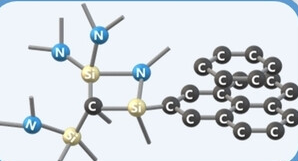
\includegraphics[width=\marginparwidth]{figures/application3/image1.png}
}

The precence of both carbon-carbon and silicon-nitrogen bond give to the material the proprerties of electronic conductivity, hardness and has a lower bindig energy of the physisorbtion process for the Na cation compare to carbon (ref Sodiophilicity/potassiophilicity chemistry in odium/potassium metal anodes, Xian Chen 2020). This material is in comparison with hard carbon, also obtained by pyrolisis of carbonacious precursors in inert atmosphere, which exhibits good mechanical properties and electrical conduction. This class of material exibits low density and and high microporosity make them excelent candidates for the storage of cation. Hard carbons are widelly used as negative electrodes in lithium and sodium ion batteries while the silicon carbonitride was demonstrated to give comparable capacity (ref Carbon-rich SiCN ceramics as high capacity/high stability anode material for lithium-ion batteries, Reinold et al. 2013 and Sic et al. SiCN Ceramics as Electrode Materials for Sodium/Sodium Ion Cells - Insights from 23Na In-Situ Solid-State NMR 2022). The reserach is still ongoing on the micro scale strucutring, dopoing and funzionalization fo these materials to increase the storage capacity (ref Enhancing the performance of hard carbon for sodium-ion batteries by coating with silicon nitride/oxycarbide nanoparticles, Hang Cheng et al 2021, Understanding of the sodium storage mechanism in hard carbon anodes, Chen et al. 2022)

Silicon carbonitride, for the presence of Si-N bonding should a particularly good binding energy with atomic sodium, favorating the electrodeposition in the pore of the material. Marco Melzi et al demonstrated an increase of capacity when allowing the lower voltage limit to negative values, i.e. allowing electroceposition of Na to happen with high efficiency. Reducing the micro-porosity during the synthesis step removes the gain in performance. The goal of the project here describe was to find evidences of metal plating through the impedance during reduction and help infering the mechanism.


\subsubsection{Speculations on storage mechanisms}

\marginpar{
    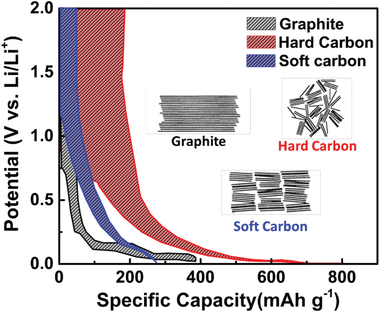
\includegraphics[width=\marginparwidth]{figures/application3/image2.png}
}

Multiple mechanisms are responsible for the storage of cation in the micro-porosity of the materials. Figure XX shows the different in the material potential vs Li during reduction of the electrodes. It is clear the absents of plateau which are associated with a phase change of a crystalline ordered structure, absent for the case of disordered carbon.
The most accredited storage mechanisms are adsorbtion, insertion and metal electrodeposition, as schematized in the Figure.

\begin{figure}[H]
    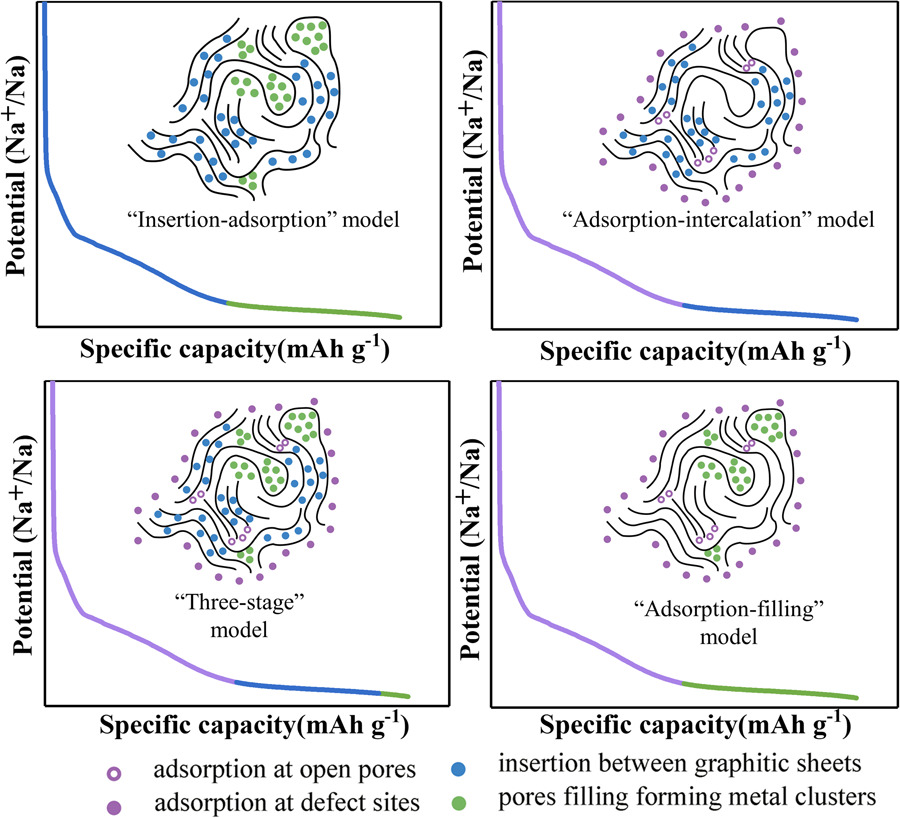
\includegraphics[width = \linewidth]{figures/application3/image3.png}
\end{figure}

It is still an open question which of this processes contribute the most and at which potential, and important information to design materials with higher capacity. Multiple theories are taken into account to far as reported in Figure.

\begin{figure}[H]
    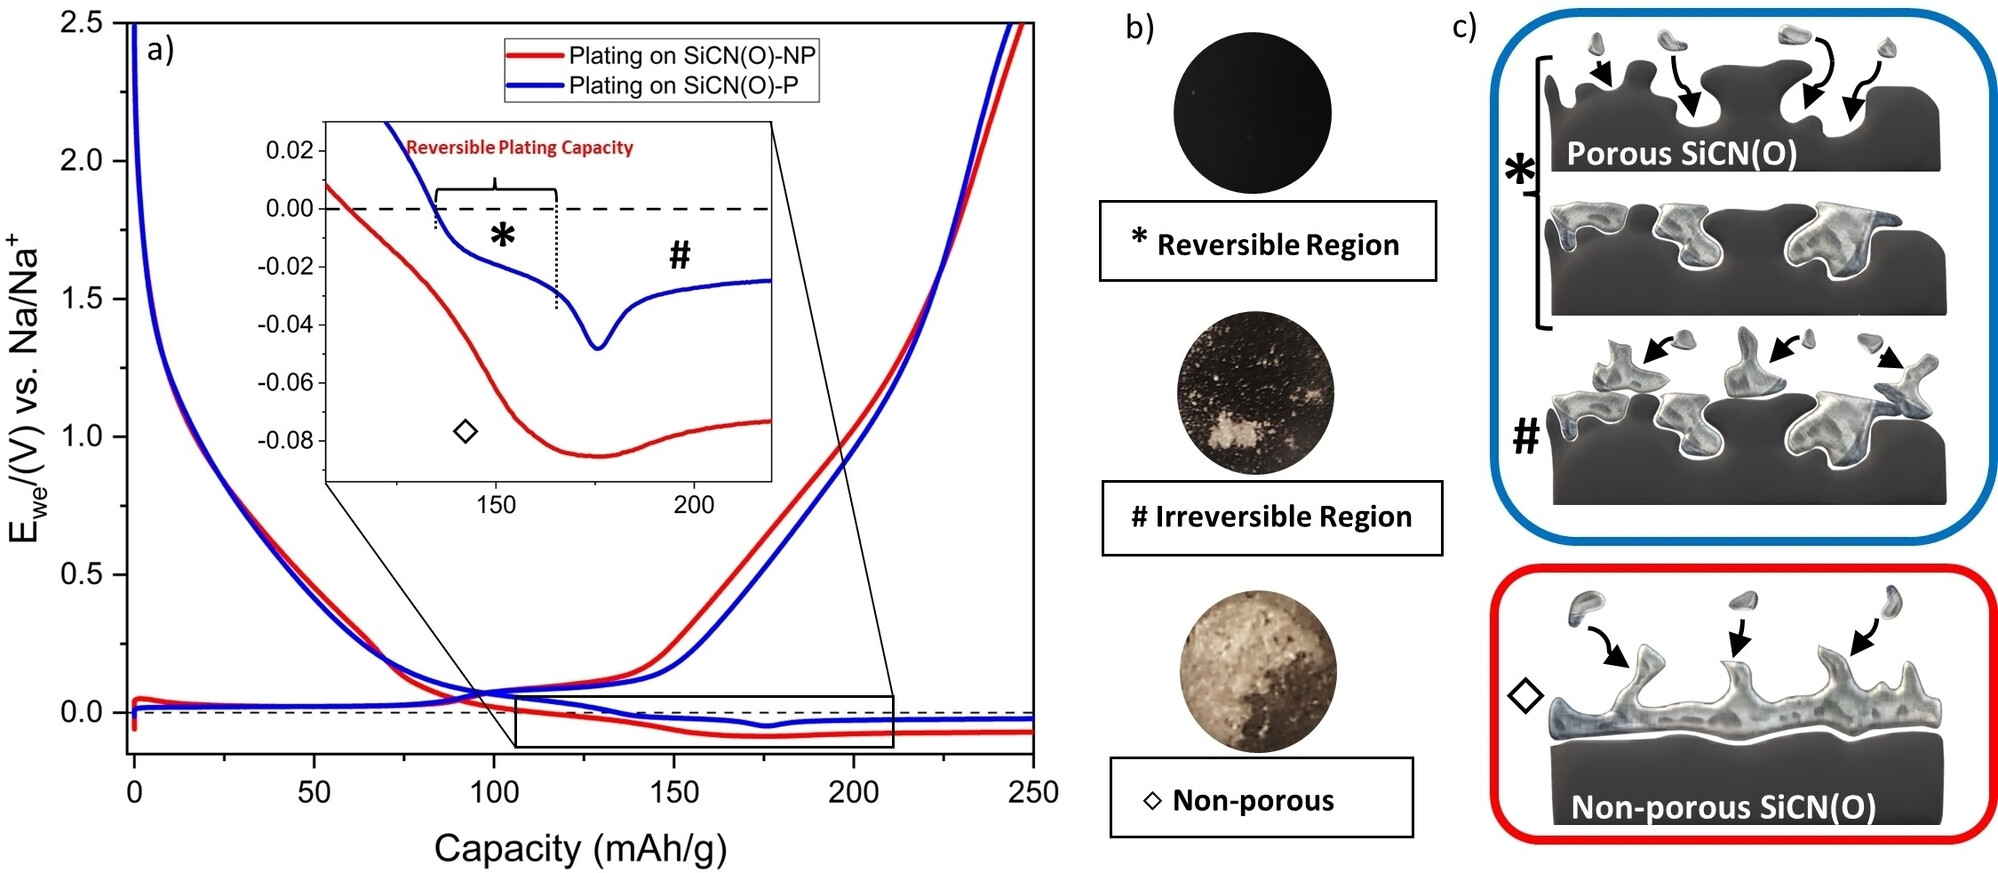
\includegraphics[width = \textwidth]{figures/application3/image4.png}
\end{figure}

Study such characteristics can only be done in operando condition with in situ tehcniques. Reserached used different mothodology for the identification of the position of the cation in the strucutre such as Nuclear Magnetic Resonance and Raman Spectroscopy. 

The scope of the measurements presented here is to veify if DEIS is capable of identify the Sodium storage mechanisms among the proposed models and support the claim about reversible metal deposition in the pores of the microstructured SiCN(O), deduced initially from the high efficiency of galvanostatic cycling.

\section{Electrode preparation and cell assembling}

\subsection{Graphite electrode}
An acqueous slurry of graphite AF-261 with 6\% SuperP C60 to increase electronic conductivity and 3\% Carboxymethylcellulose as binder. 
The slurry is casted on Copper foil with an automatic machine and cut in squares of 2cm side, vacuum dried at 80°C overnight.

\subsection{SiCN(O) electrode}
The SiCN(O) electrodes were prepared from powder (particle size 40$\mu$m) mixed with 2\%w Carbon Black for enhance conductivity and 2\%w Carboxymethylcellulose and 2\%wStyrene Butadiene Rubber as binders. 
An acqueous slurry is casted on Alluminum foil, which is then cut into 12mm disks and vacuum dried at 80°C for 24 hours.
The information on the synthesis route of SiCN(O) are found in [MdE On the reversible sodium plating], as well as details on the electrode composition and characterization.

\subsection{Metallic sodium}
Discs of 12mm with sodium on alluminum. They come from a supplier with flat surfaces and protective plastic foils on both sides.

\subsection{Electrolyte}
1M LiPF6 in EC:DEC 1:1w with 2\%w VC for graphite/lithium cells and 1M NaPF6 in EC:DEC 1:1w for the SiCN(O) and Sodium. 

\subsection{Micro-reference electrodes}
% Fabrication
% Types of substrates
% Expected stability
% Issues (geometry, metal dissolution)

Microscopic reference electrode introduced in pouch cells are made out of an insulated metallic wire with the section esposed. 
This concept is the closest realization of a punctual electrode. 
\marginpar{
    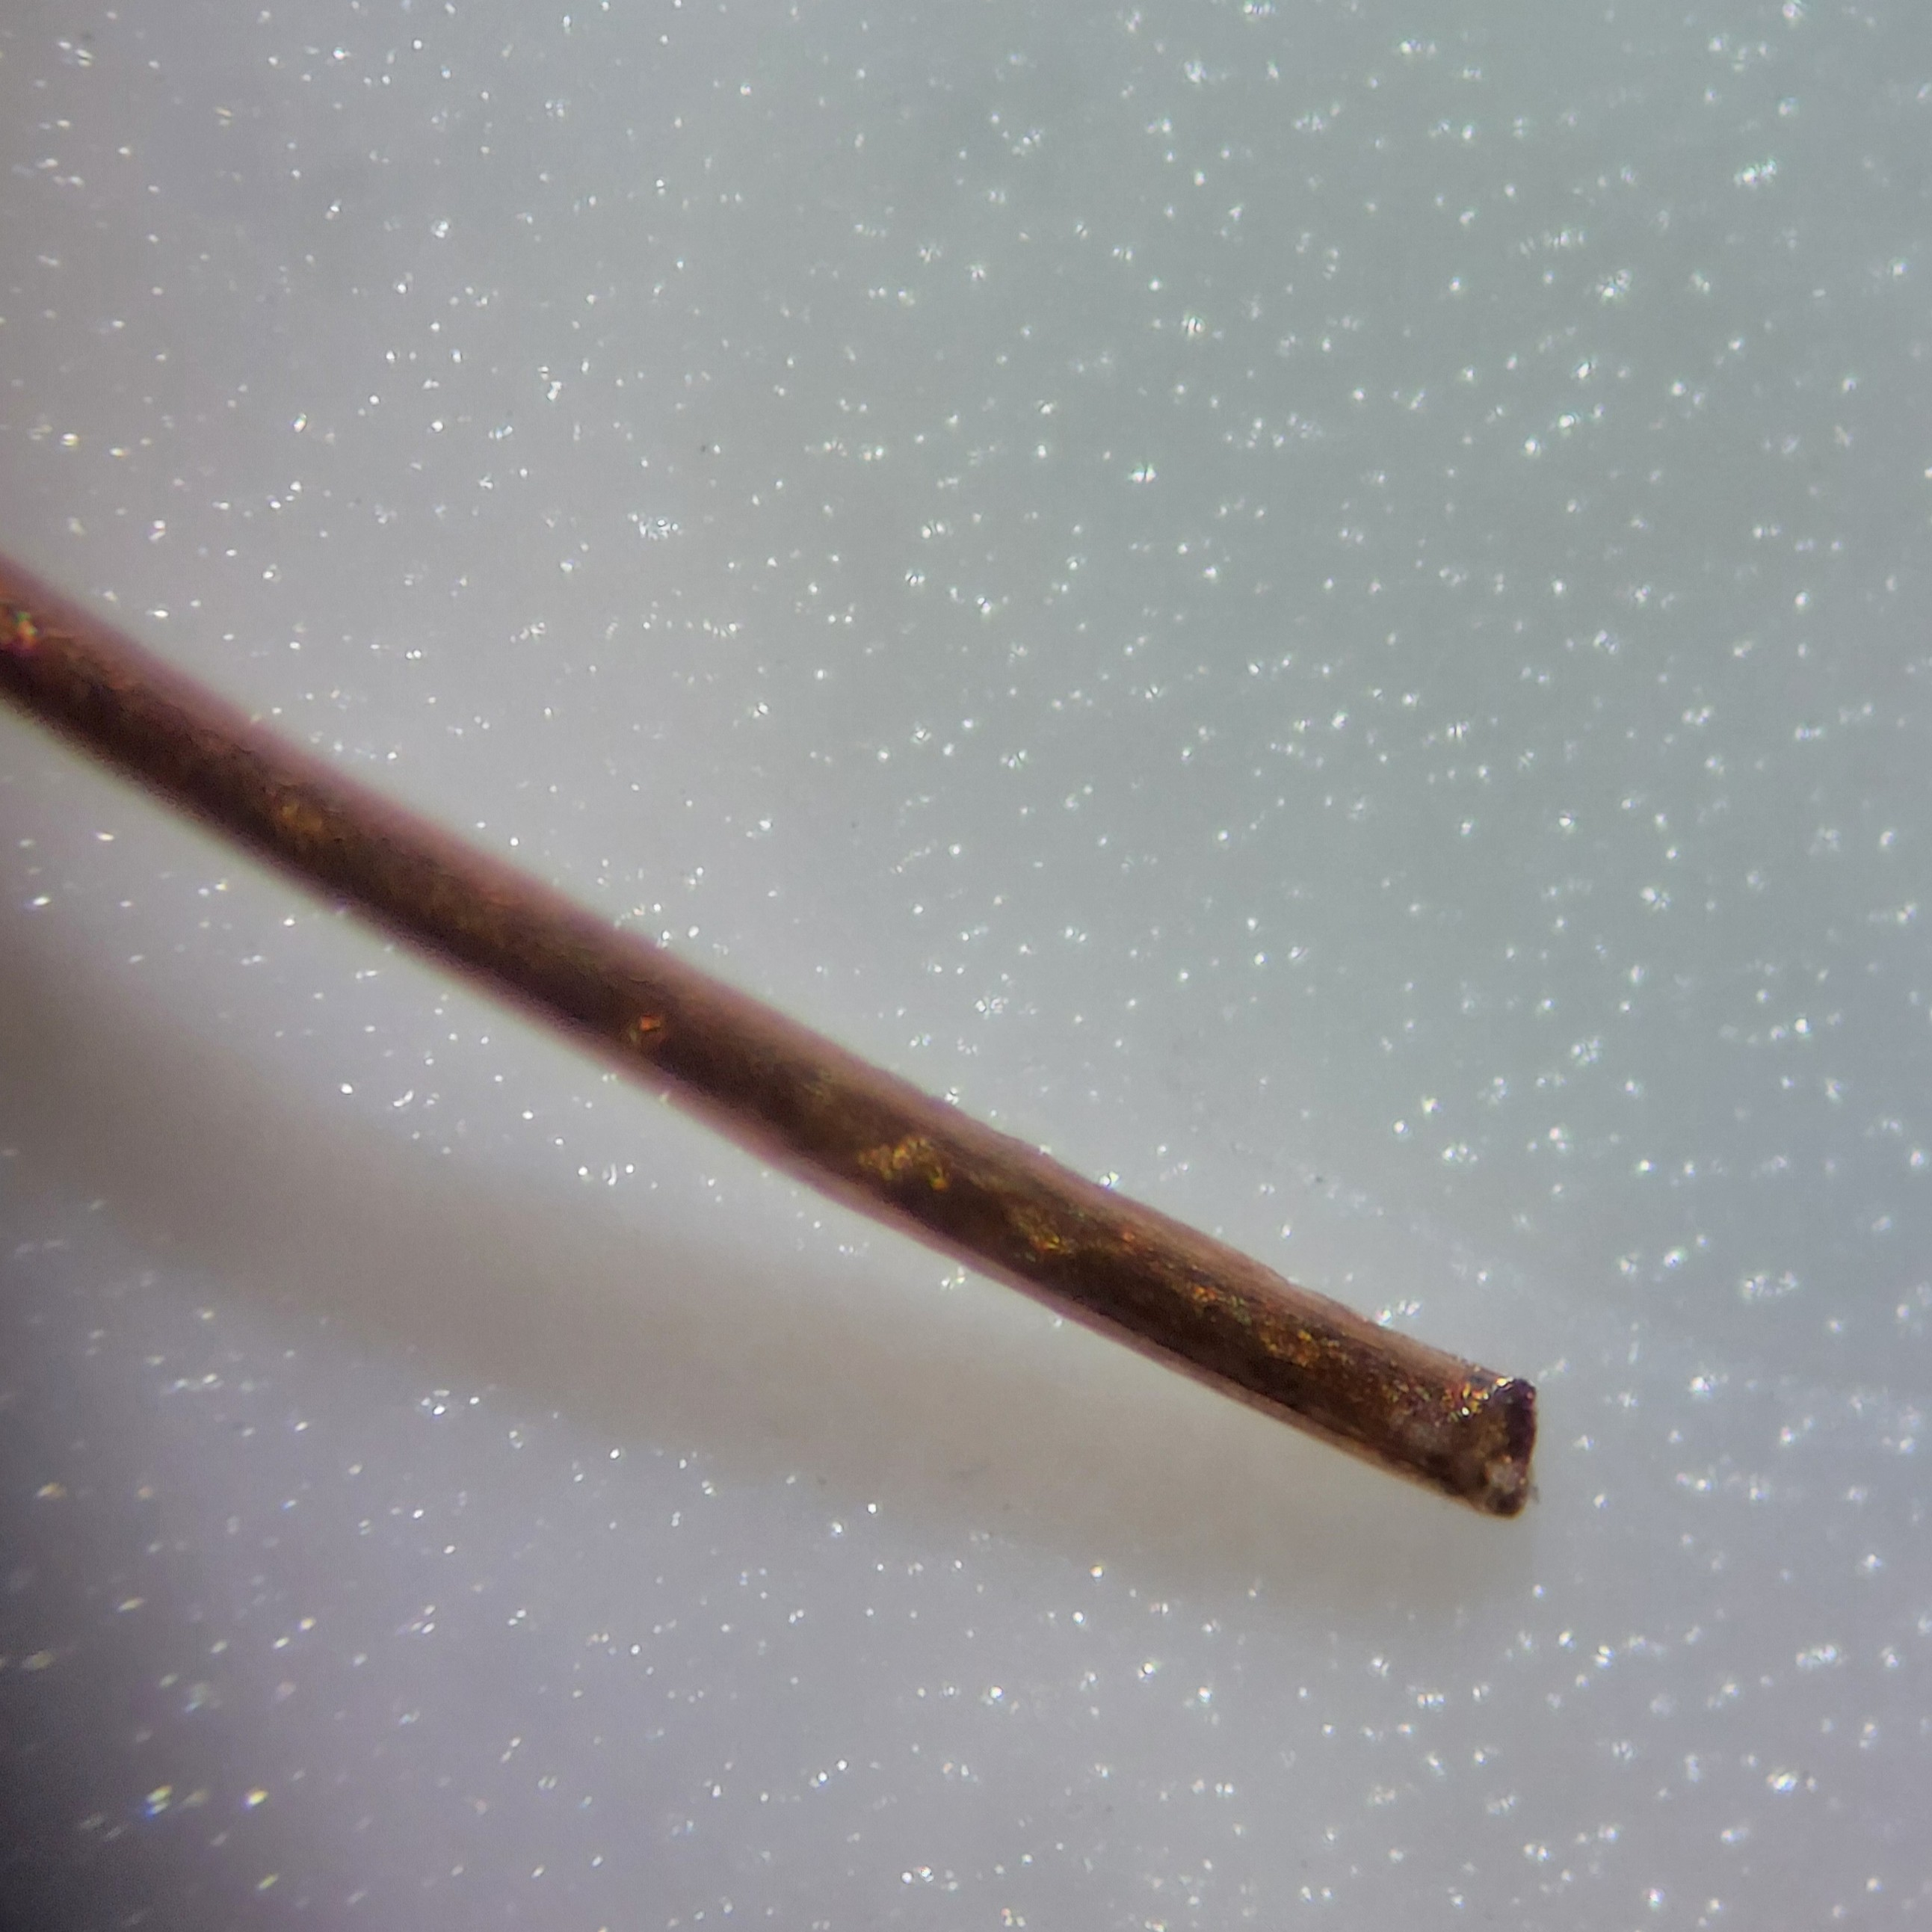
\includegraphics[width=\marginparwidth]{figures/anodes/copper_wire_microscope.jpg}
}
The goal is to being able to probe the local potential in only one point where the field lines are equipotential.
In this work I used three types of insulated wires:
\begin{itemize}
    \item circa 130$\mu$m copper manually insulated with termosetting polymer strips.
    \item 50$\mu$m diameter polymer insulated Copper from Goodfellow;
    \item 50$\mu$m diameter polymer insulated Gold from Goodfellow;
\end{itemize}
I want to explain better the last electrode support. 
I took a copper wire from a woven desoldering cloth and used the polymeric thermosetting strips used for sealing pouch cells to cover the wire.
Figure \ref{fig:microref_wires} shows the components used to assemble the wire and the comparison with the commercial one.
\begin{figure}[H]
    \centering
    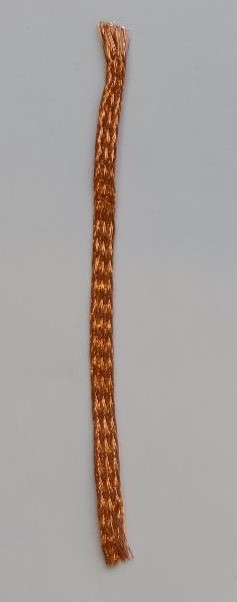
\includegraphics[width=2cm]{figures/application3/image5.1.jpg}
    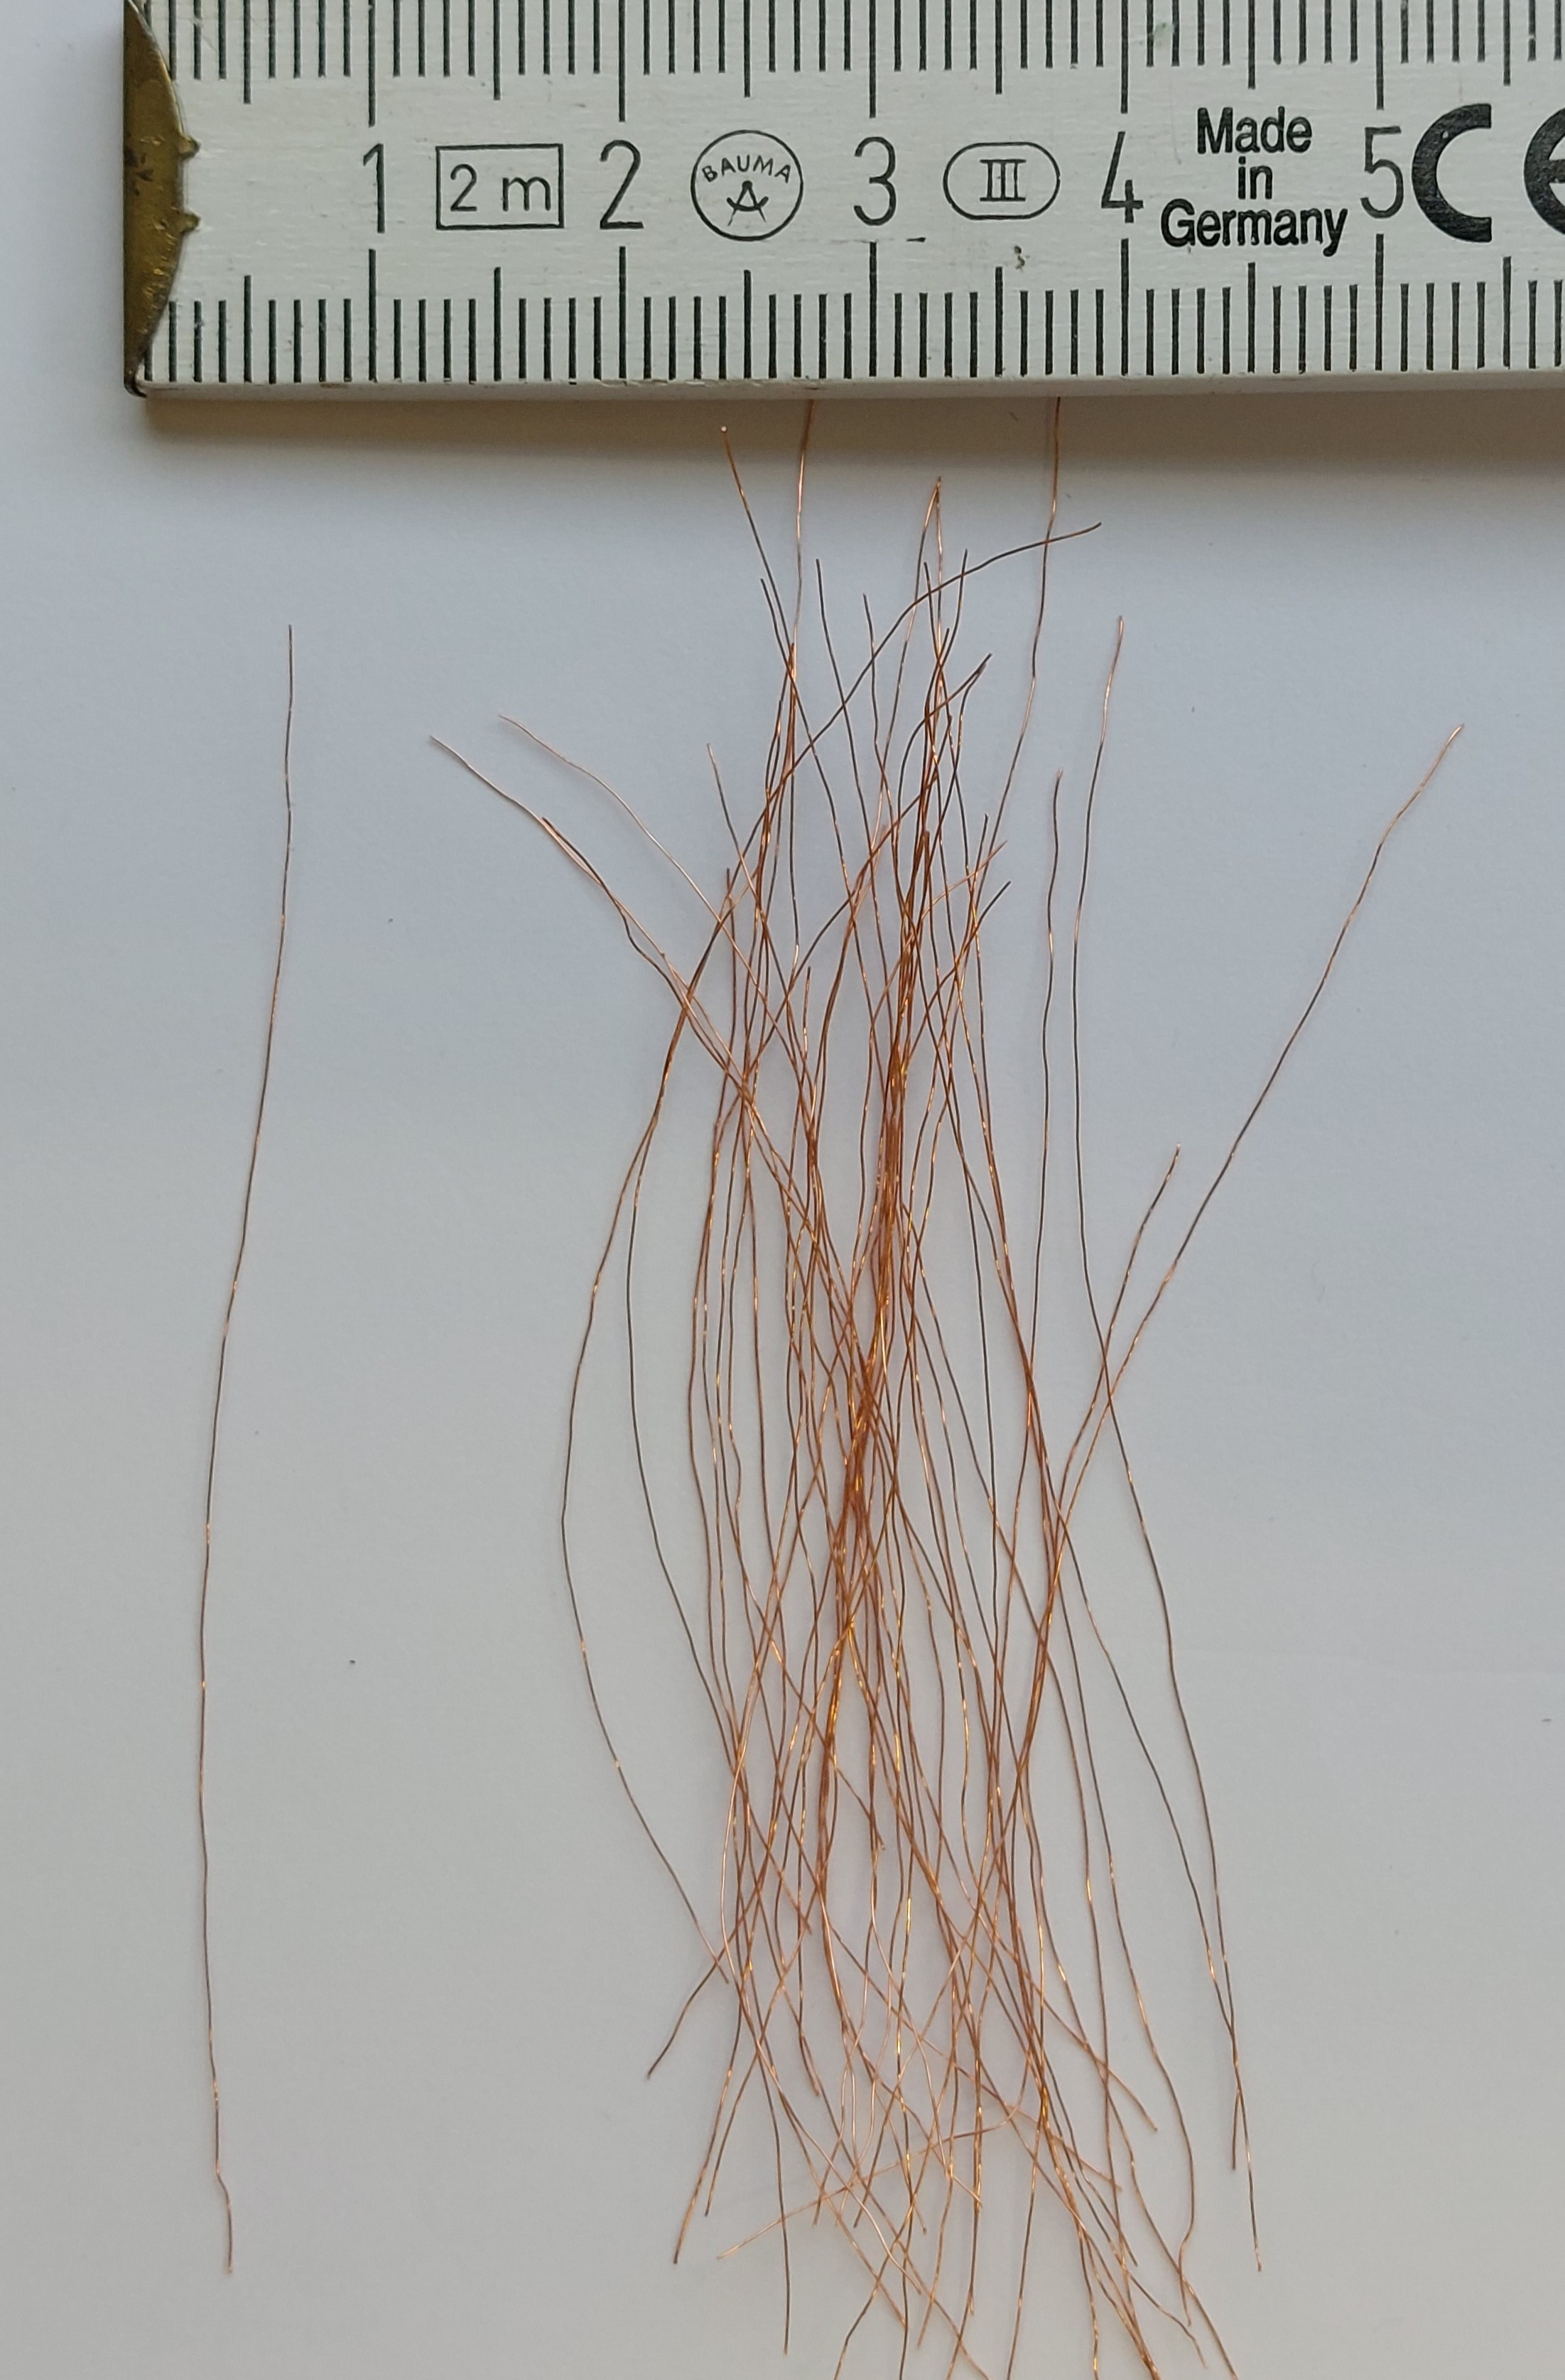
\includegraphics[width=2.5cm]{figures/anodes/unwoven_copper_wires.jpg}
    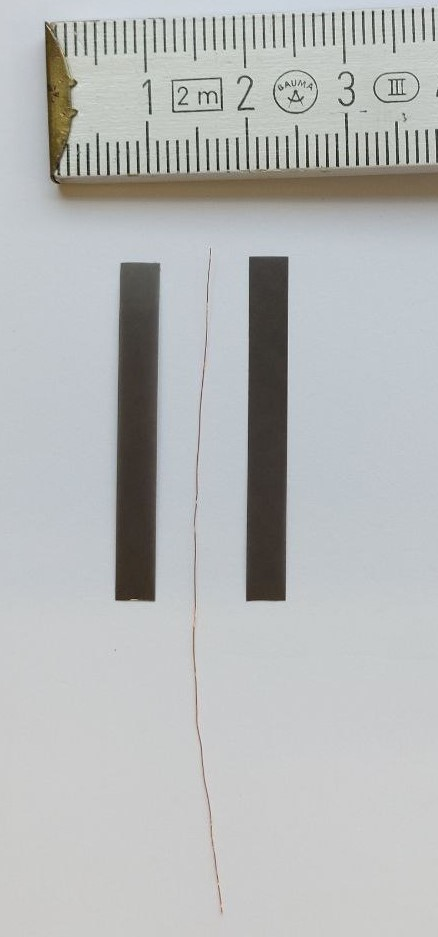
\includegraphics[width=2cm]{figures/application3/image5.2.jpg}
    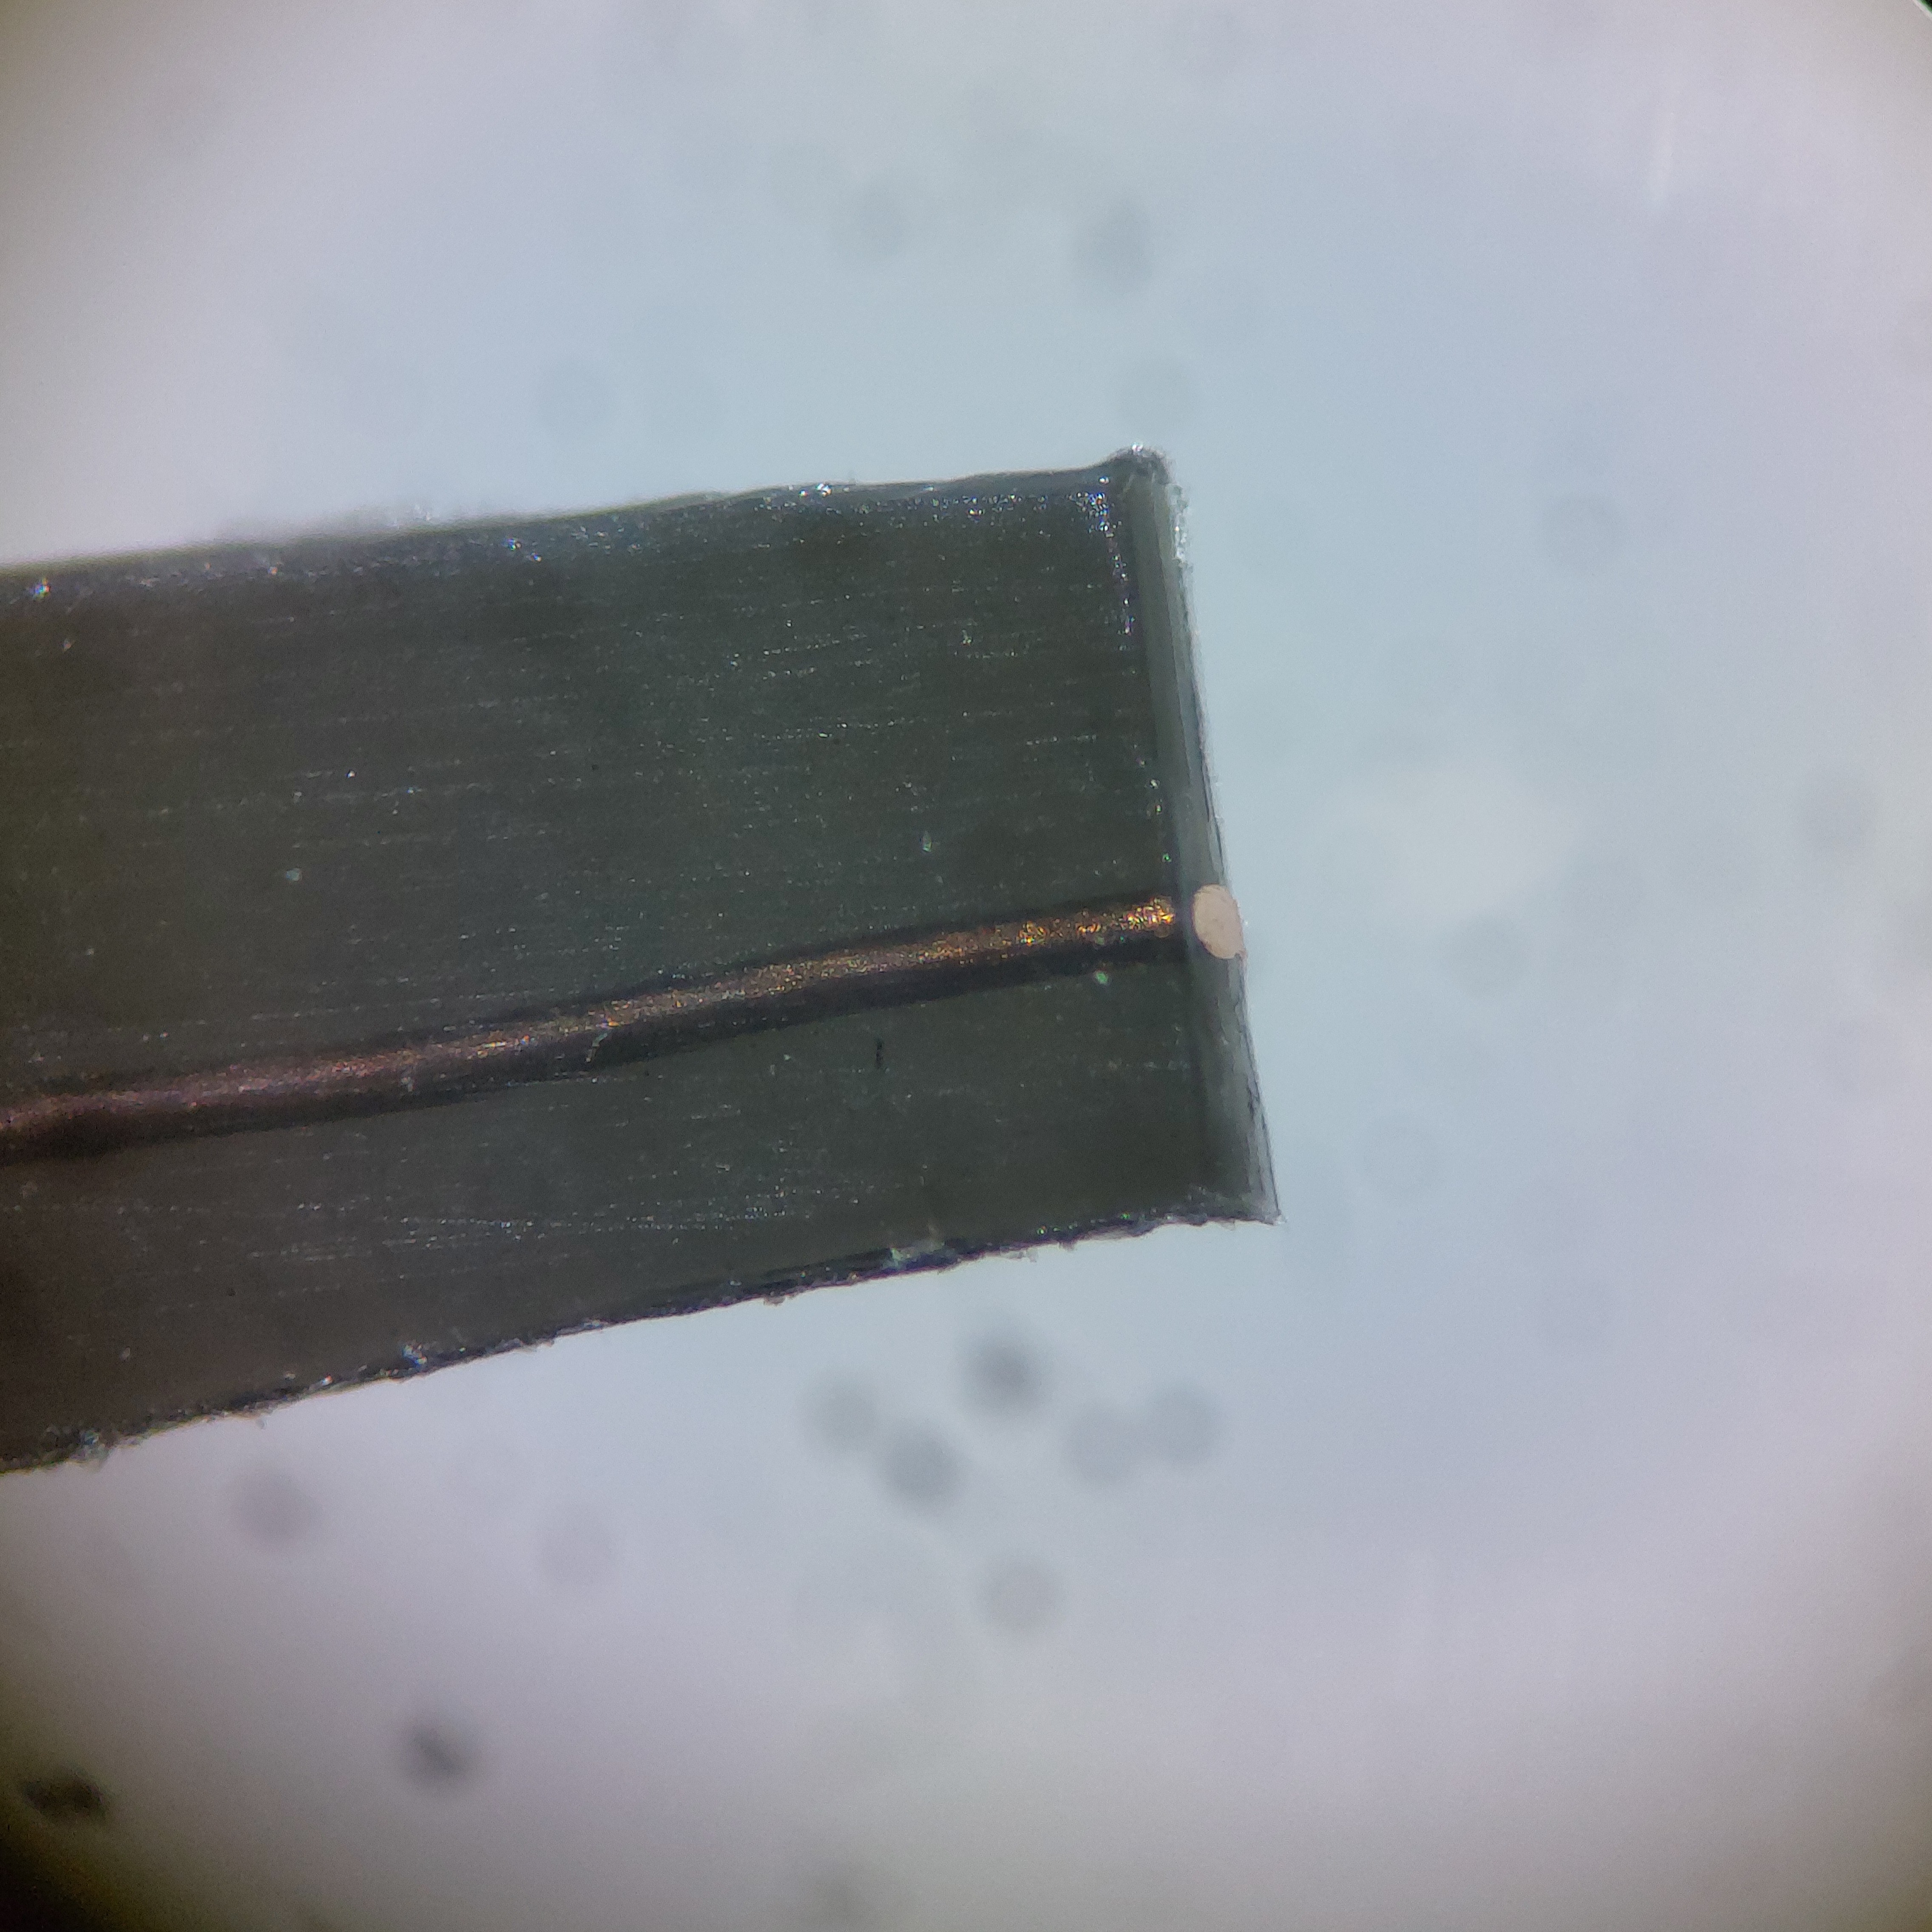
\includegraphics[width=4cm]{figures/anodes/copper_130um_insulated.jpg}
    \caption{From left to right: step for the preparation of insulated copper wire.}
    \label{fig:microref_wires}
\end{figure}
\marginpar{
    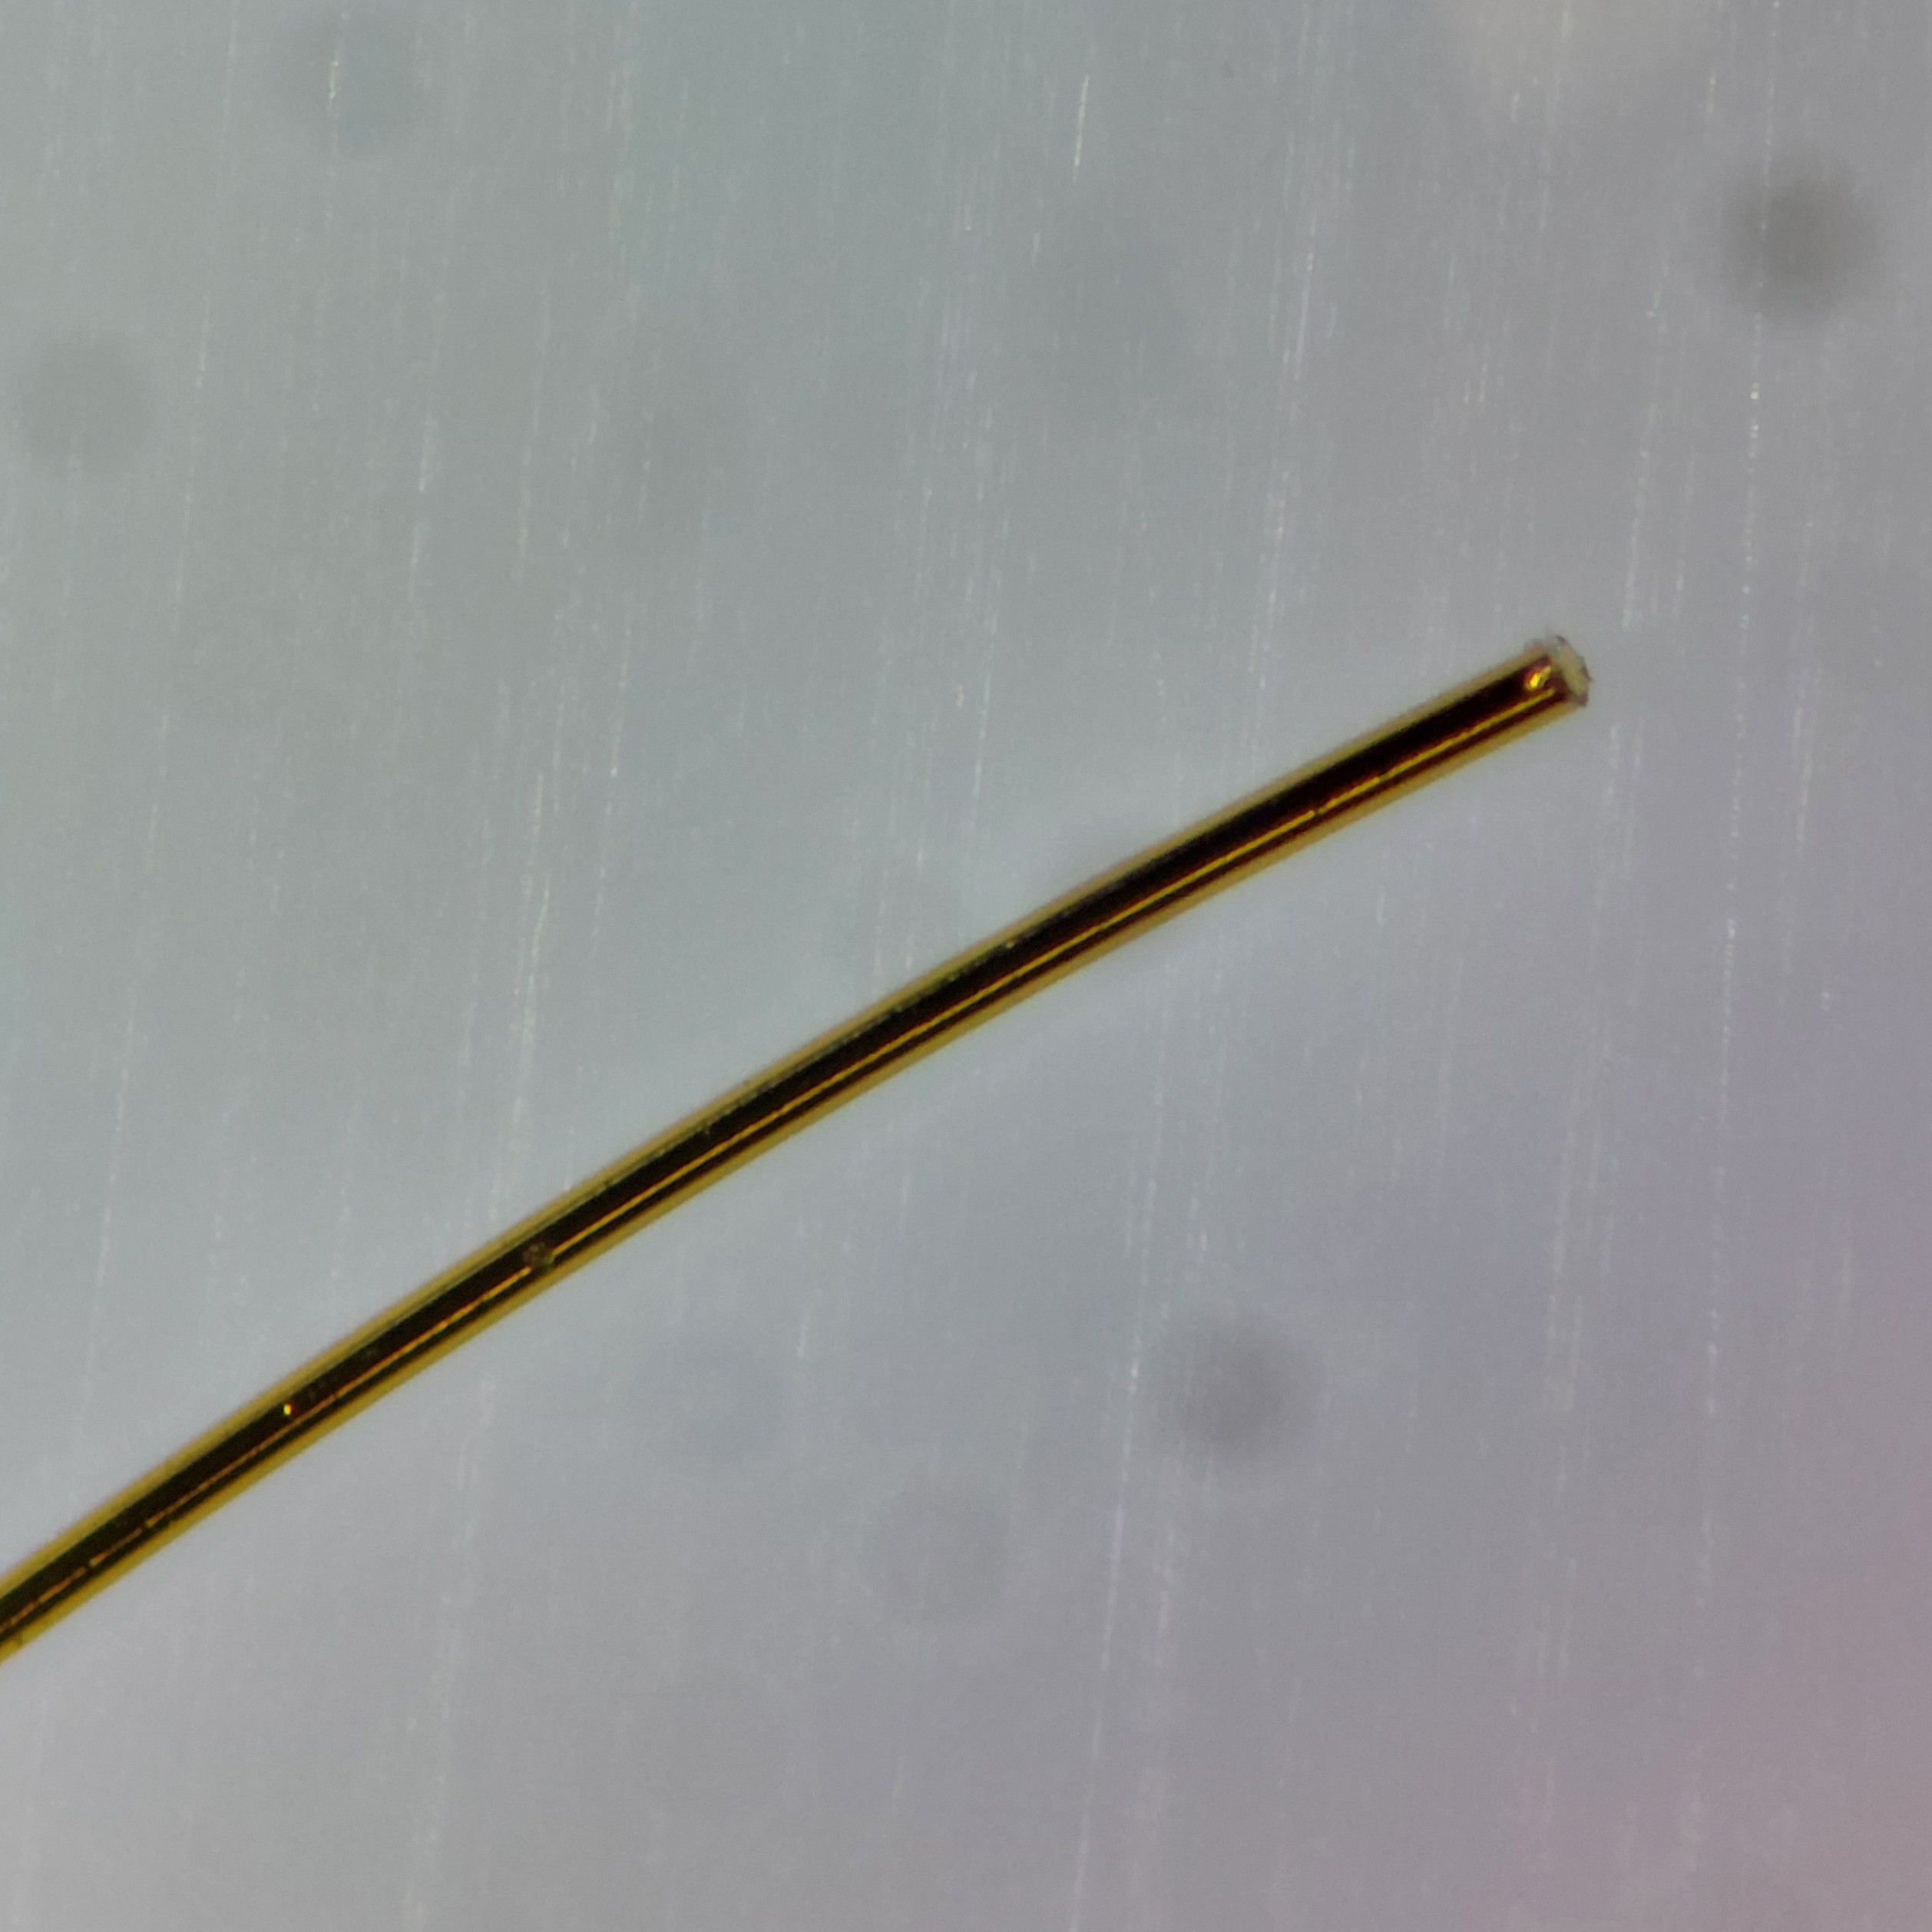
\includegraphics[width=\marginparwidth]{figures/anodes/gold_wire_microscope_better.jpg}
}
The commercial 50$\mu$m is to thin to clamp to potentiostat crocodile clamps and also prone to brake when sealed though the pouch cell foils. 
The solution (cite paper) is to scrap the insulation of the wire at one end and solder it to a peace of metal to act as current collector. 
In the paper they use the machine to solder the contact in micro-electronics which I didn't have at disposal. 
Instead I tried with the ultrasonic woldering with poor reproducibility even with the best setting I could find. 
Too much pressure cause the wire to brake while too little didn't solder the metals.
Reports on the attempt with this methods are found in Appendix \ref{app:ultrasonic wire soldering}
Finally I tried to put current collector and exposed wire in contect and sealed them togather with the thermosetting polymer strips.
\marginpar{
    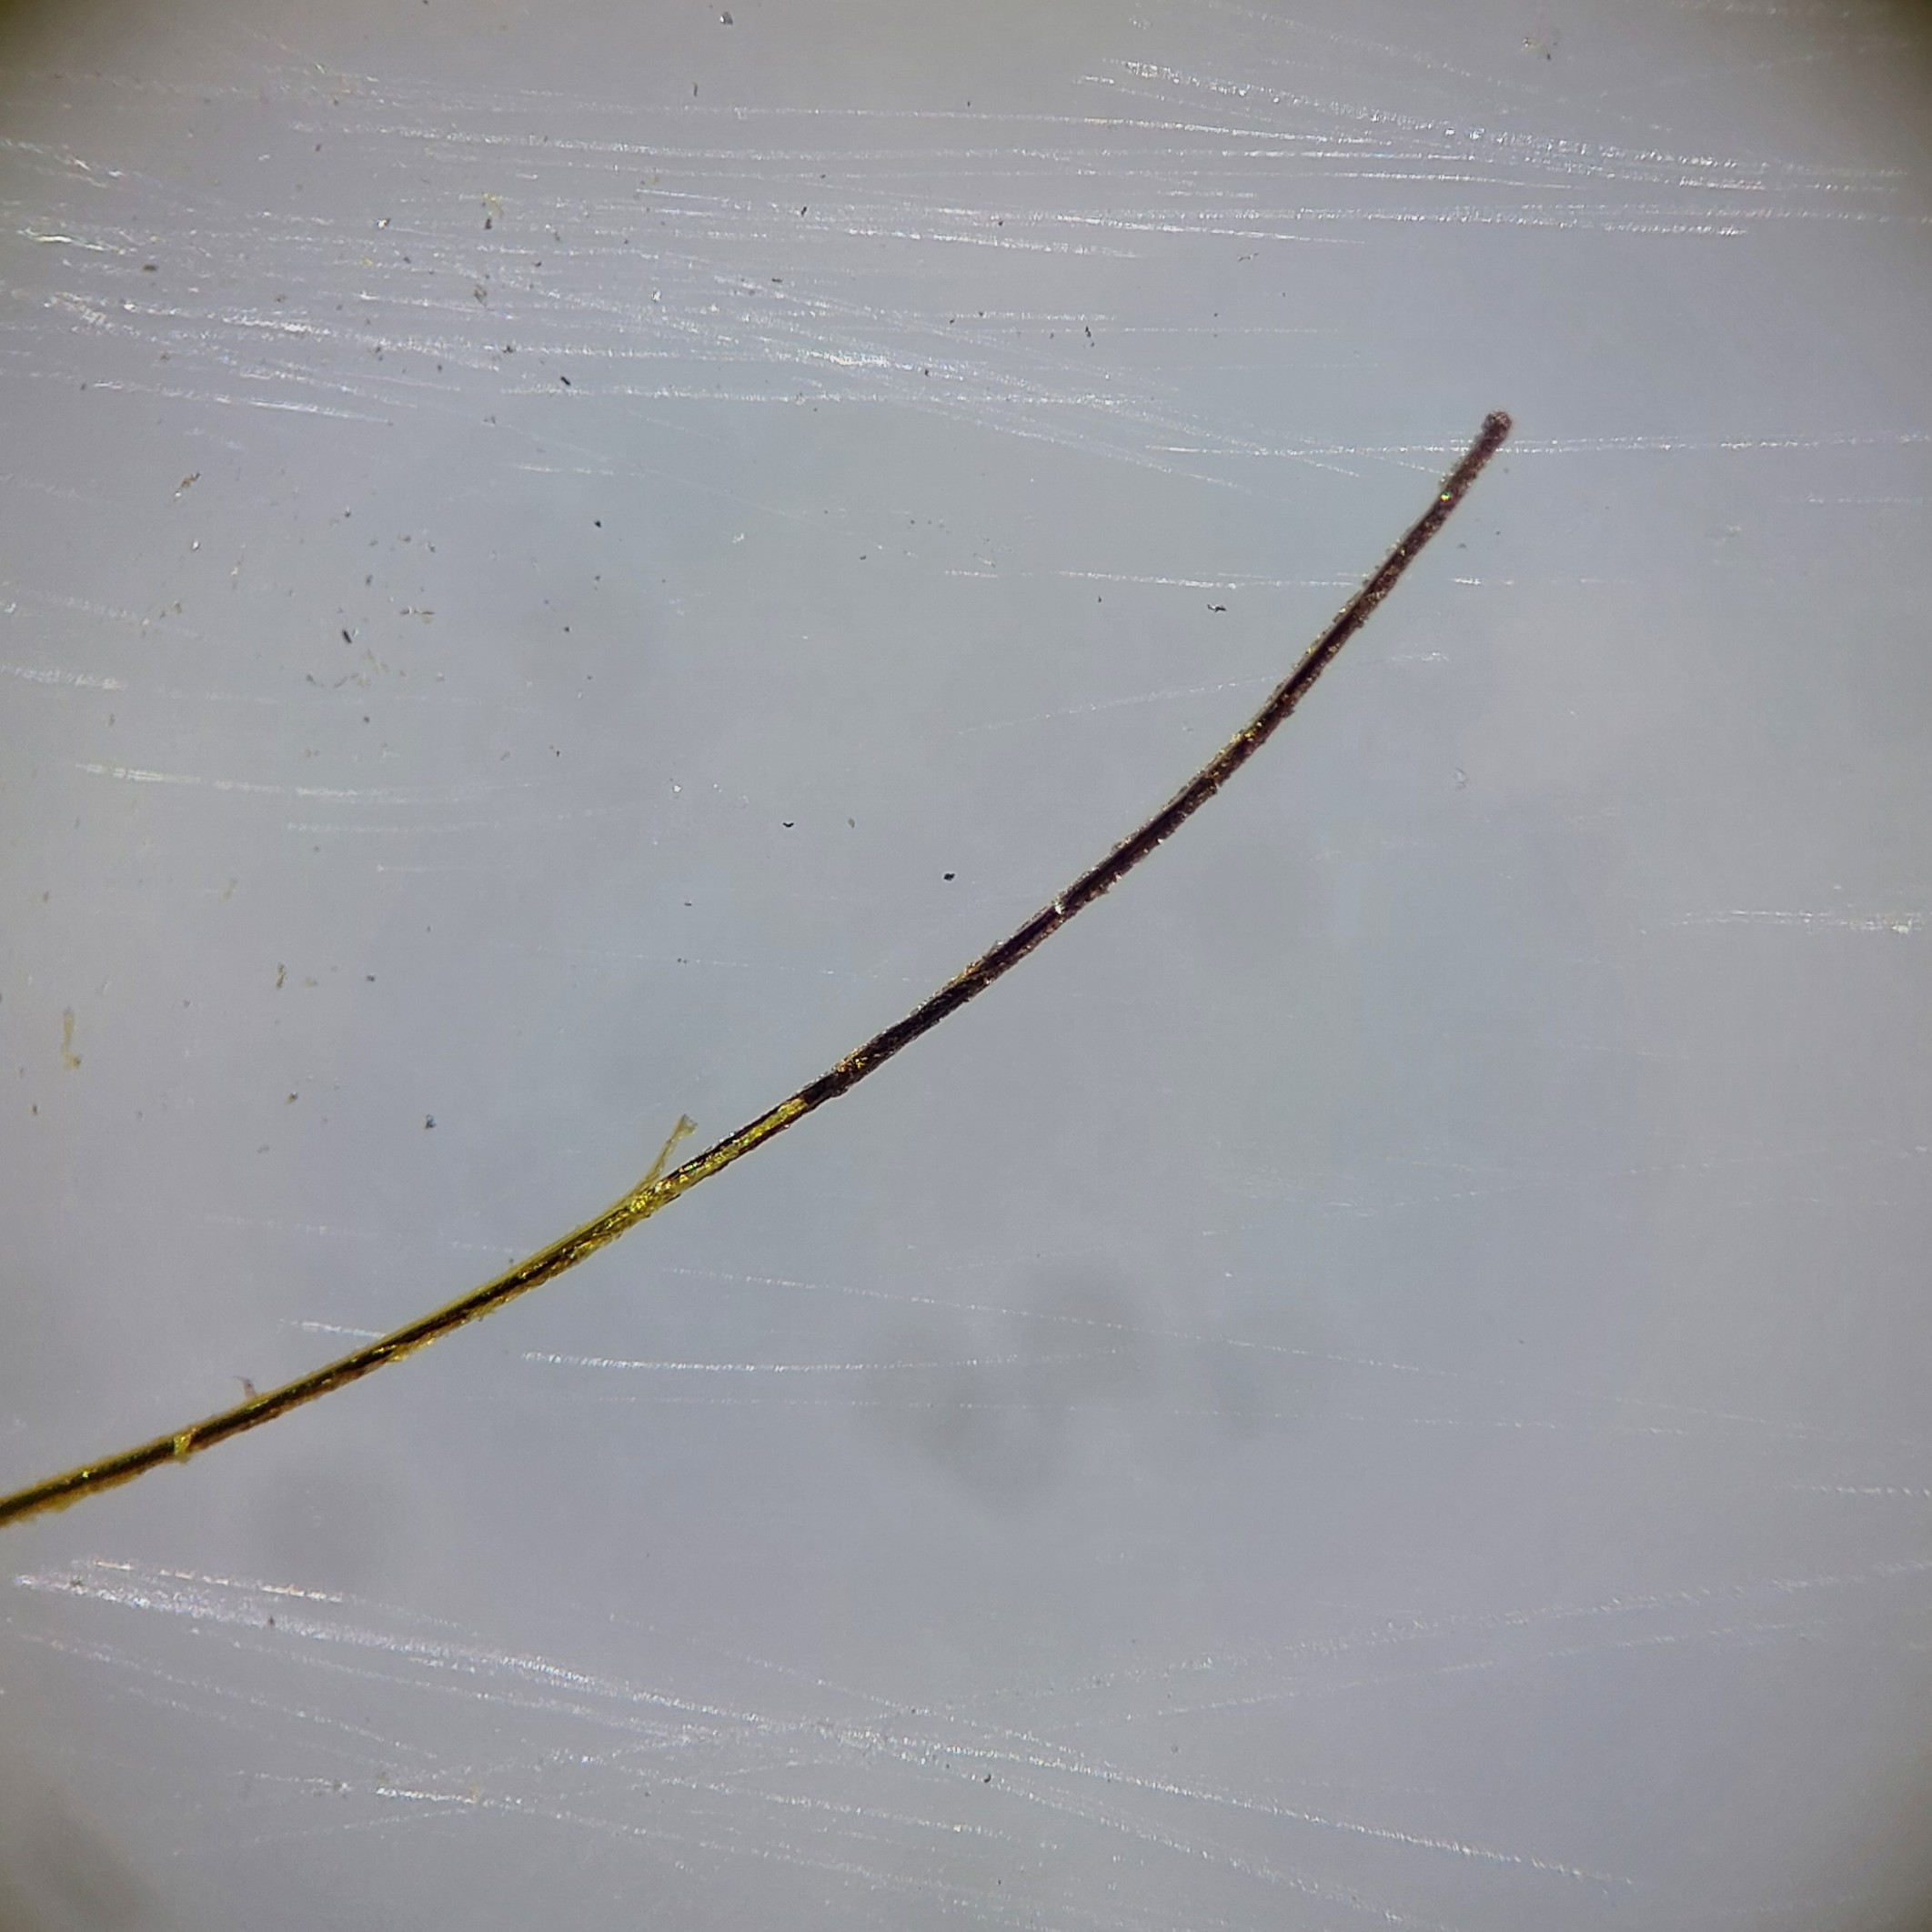
\includegraphics[width=\marginparwidth]{figures/anodes/pealed_gold_wire.jpg}
}
\begin{figure}[H]
    \centering
    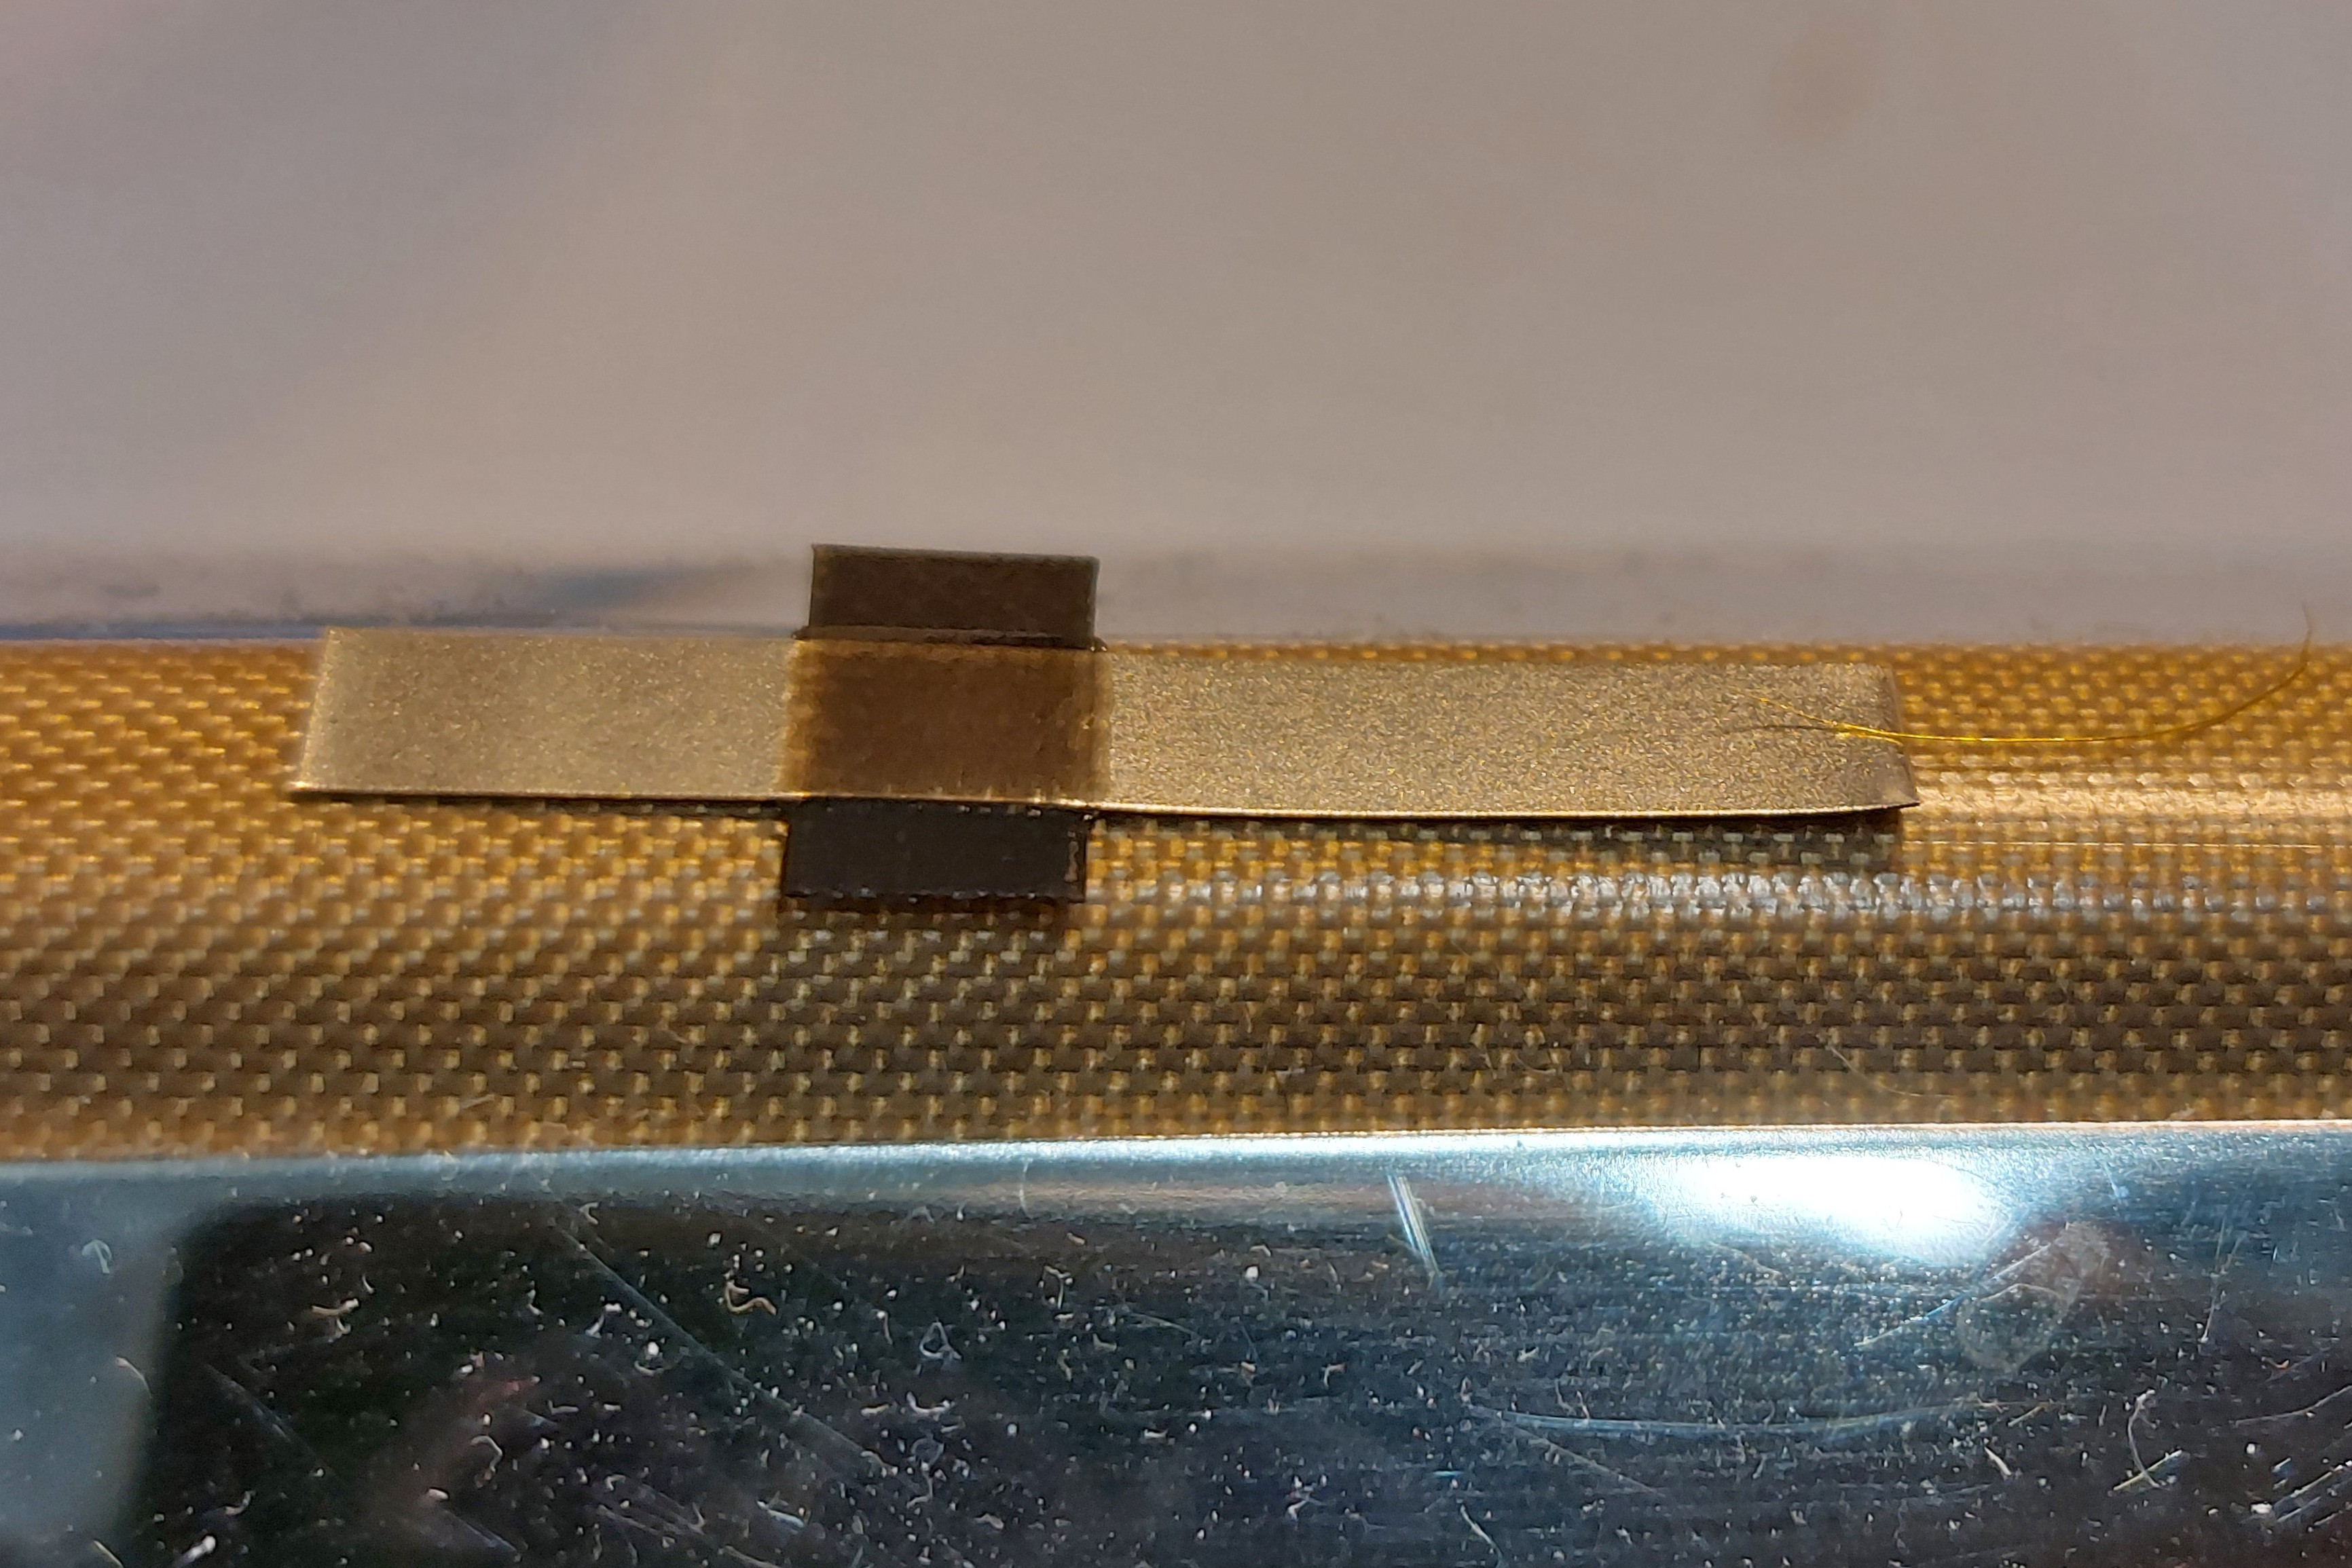
\includegraphics[width=0.4\textwidth]{figures/anodes/preparation_hadesive_bonding.jpg}
    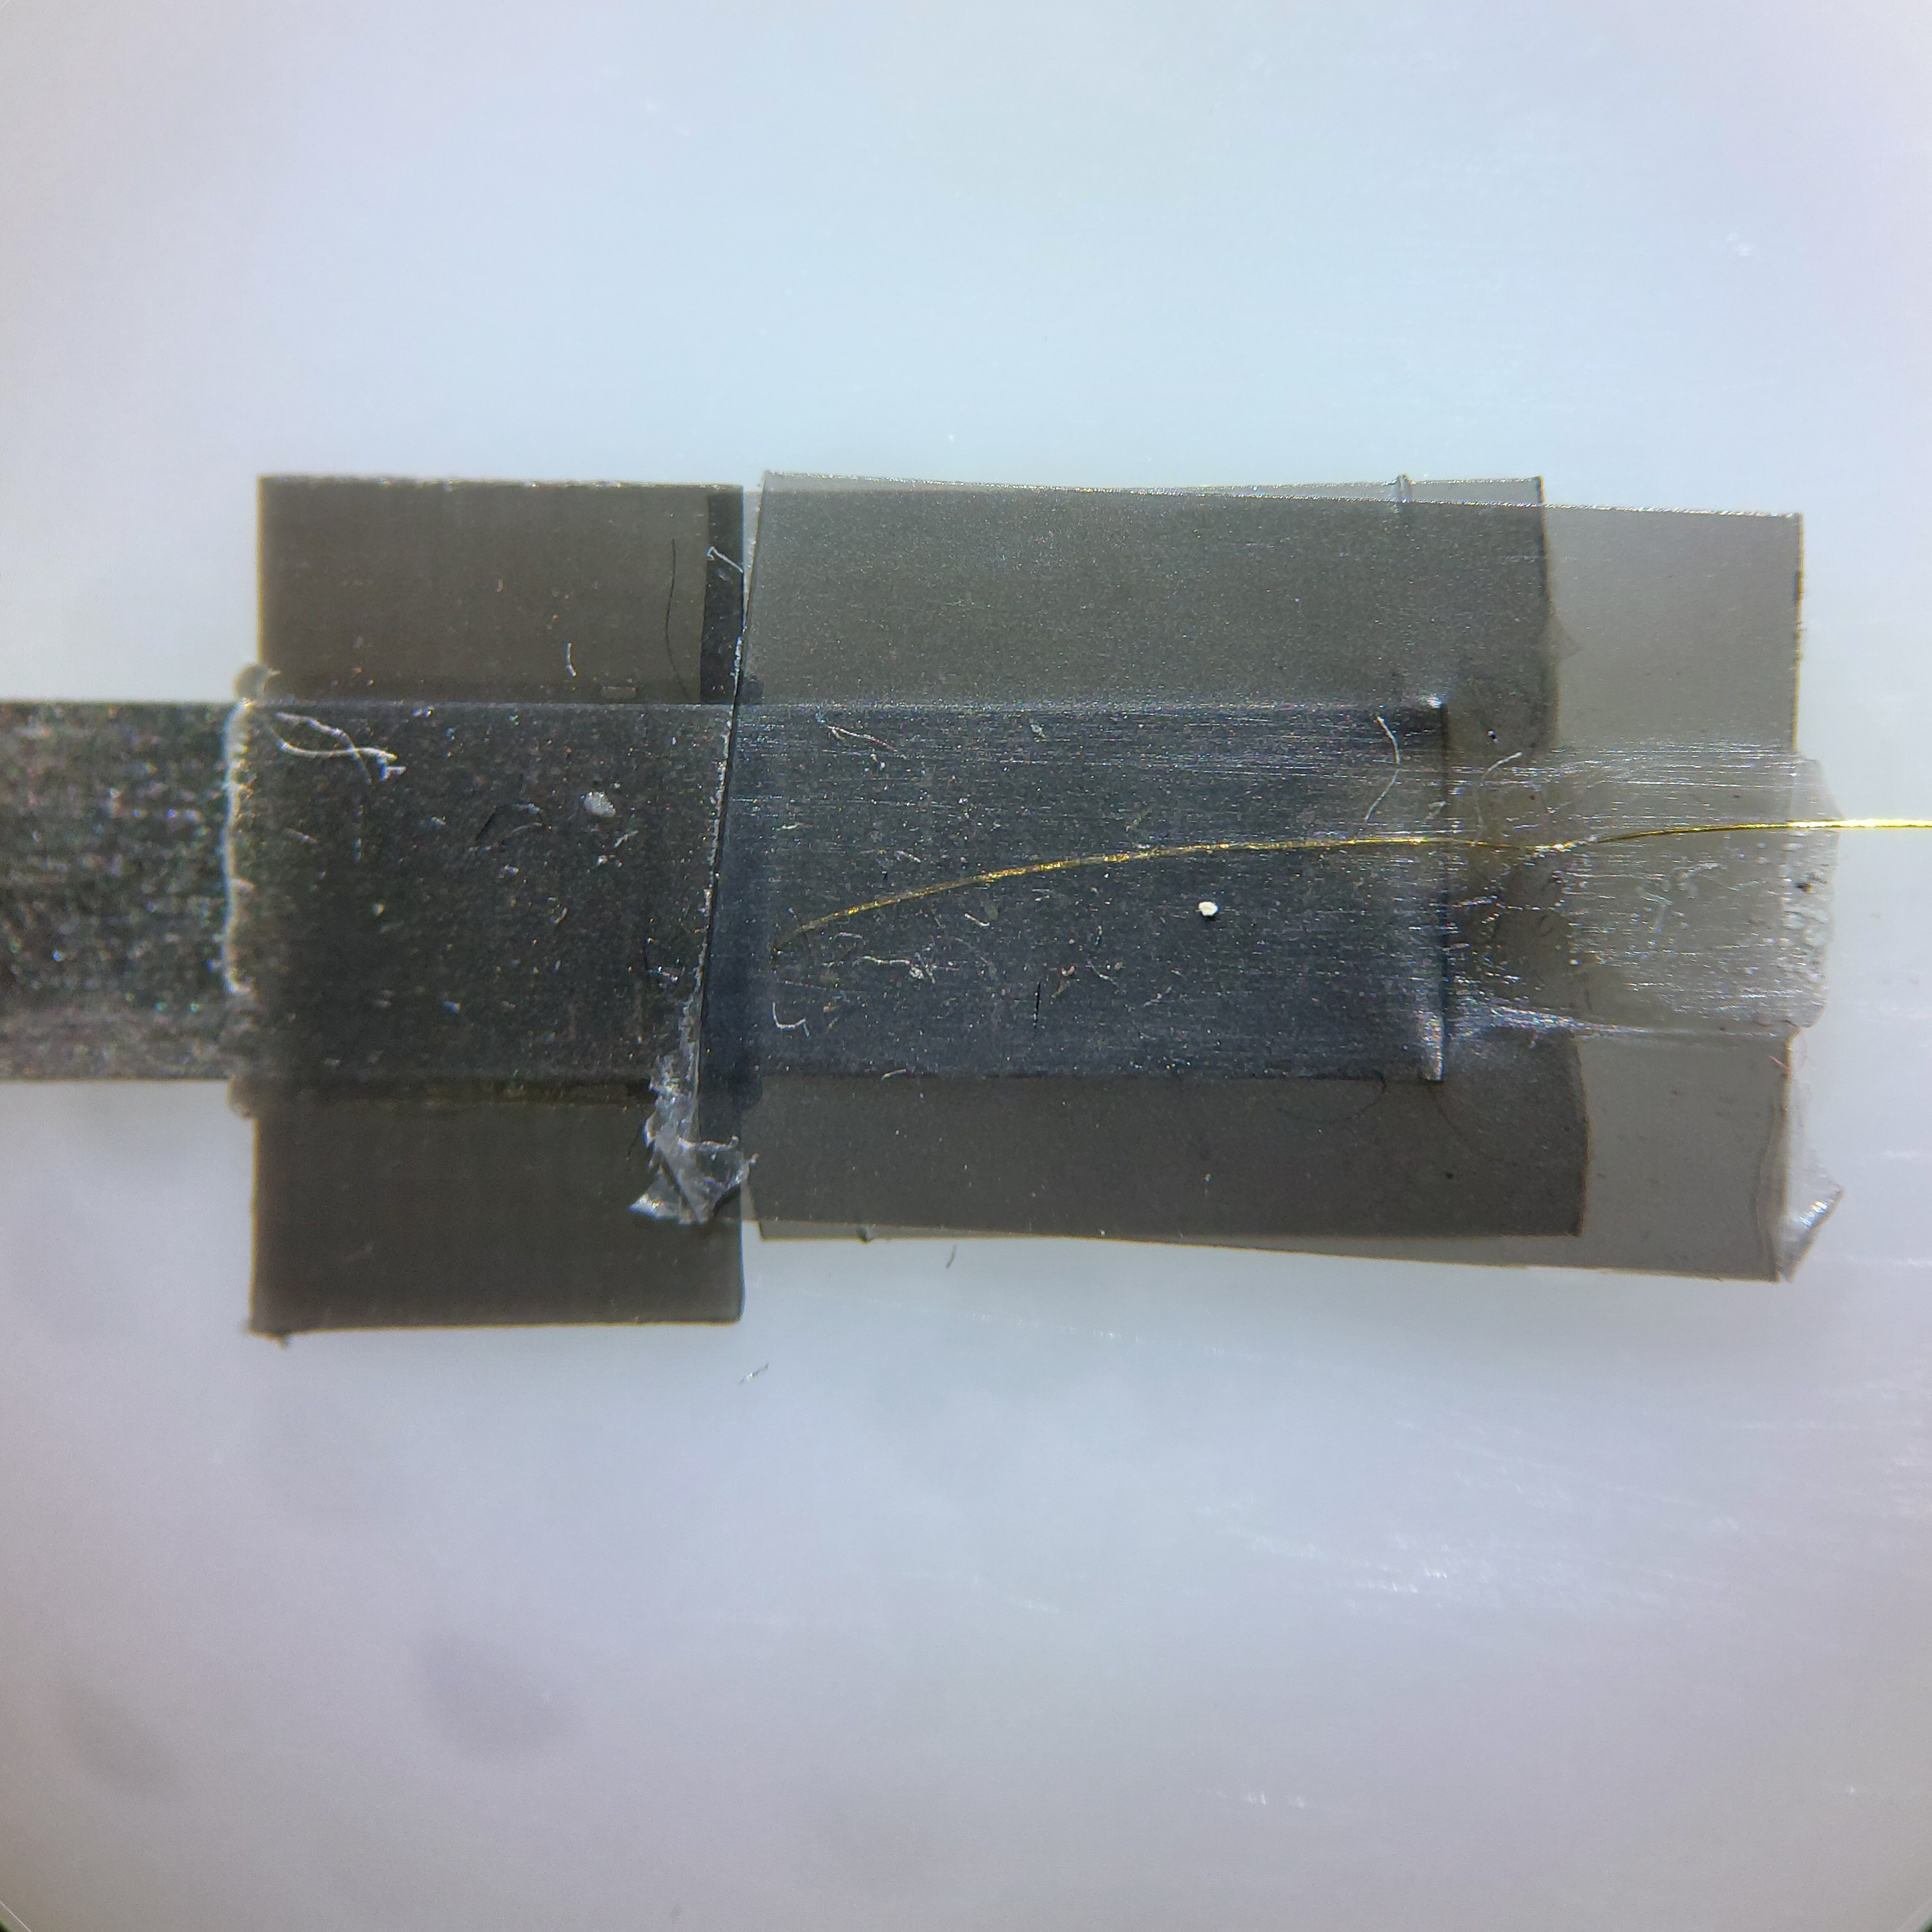
\includegraphics[width=0.25\textwidth]{figures/anodes/insulated_tab_hadesive_bonding.jpg}
\end{figure}
Although this provided electrical contact and I could performe electrodeposition of lithium with multiple techniques (CP, CA, CV), the deposited lithium was dissolving back into solution. I know this because the voltage drifts from the lithium potential to the original value of copper in a few hours (30-90). My hypotesys is that some of the current collector remain esposed and the electrodeposition happeoccours on its surface with a very low current density, not enough to form stable gems.
Furthermore the electrodeposition in organic electrolytes is cuncurrent with the degradation of the electrolyte.

The insulation of the wire was done putting the wire between to strips of polymeric strip longitudinal to the heating strip of an ultrasonic sealer for coffee bags. The Excess polymer were removed with a scalpel and a section of the wire exposed like shown in Figure XX. It takes a bit of practice to cut the section parallel to the axis and get aproximatly a circular section. Without checking on the optical microscope, one might end up with elliptical section resulted from non perpendicular cut and hence a much higher surface area.

For the electrodeposition the wire was connected to the working pole of a potentiostat using a disk of metallic lithium as counter (12 mm diameter) in a two-electrode configuration. The procedure was conducted with a two steps technique, first 10 minutes of potentiostatic set at -100mV and then 3 hours in galvanostatic with -50uA of current. It followed an open circuit technique. The reference electrode produced with such techniques were stable under parasitic  current of the potentiostat for 6 months.

Gold produces an alloy with lithium. Alloys have better defined potential compared to metallic phase and there are less problem with the SEI formation. Stable reference electrodes were reported in the literature produced by alloying at cathodic anodic current of 50pA for 1 hour. 
I could not replicate the same the processes with my electrodes, probably becuase of the ineffective insulation of the nickel tabs.

\subsection{Three-electrode pouch cell}
% Geometry for lithium and sodium
% Reference electrode placing
The cell were assembled in a similar manner with two glassfiber separators and the copper wire in between them. With the experience gained from the experiment reported in chapter \ref{chap:capacitor} and the simulation in literature, I decide to put the reference in the middle of the stack. 
This introduces the need of a microscopic reference and so the production of cell more complicated. 
Using macroscopic metallic reference electrode is much more coninient in the assemly but it introduces measurement artifacts.[Do I have an example of it?]

\begin{figure}[H]
    \centering
    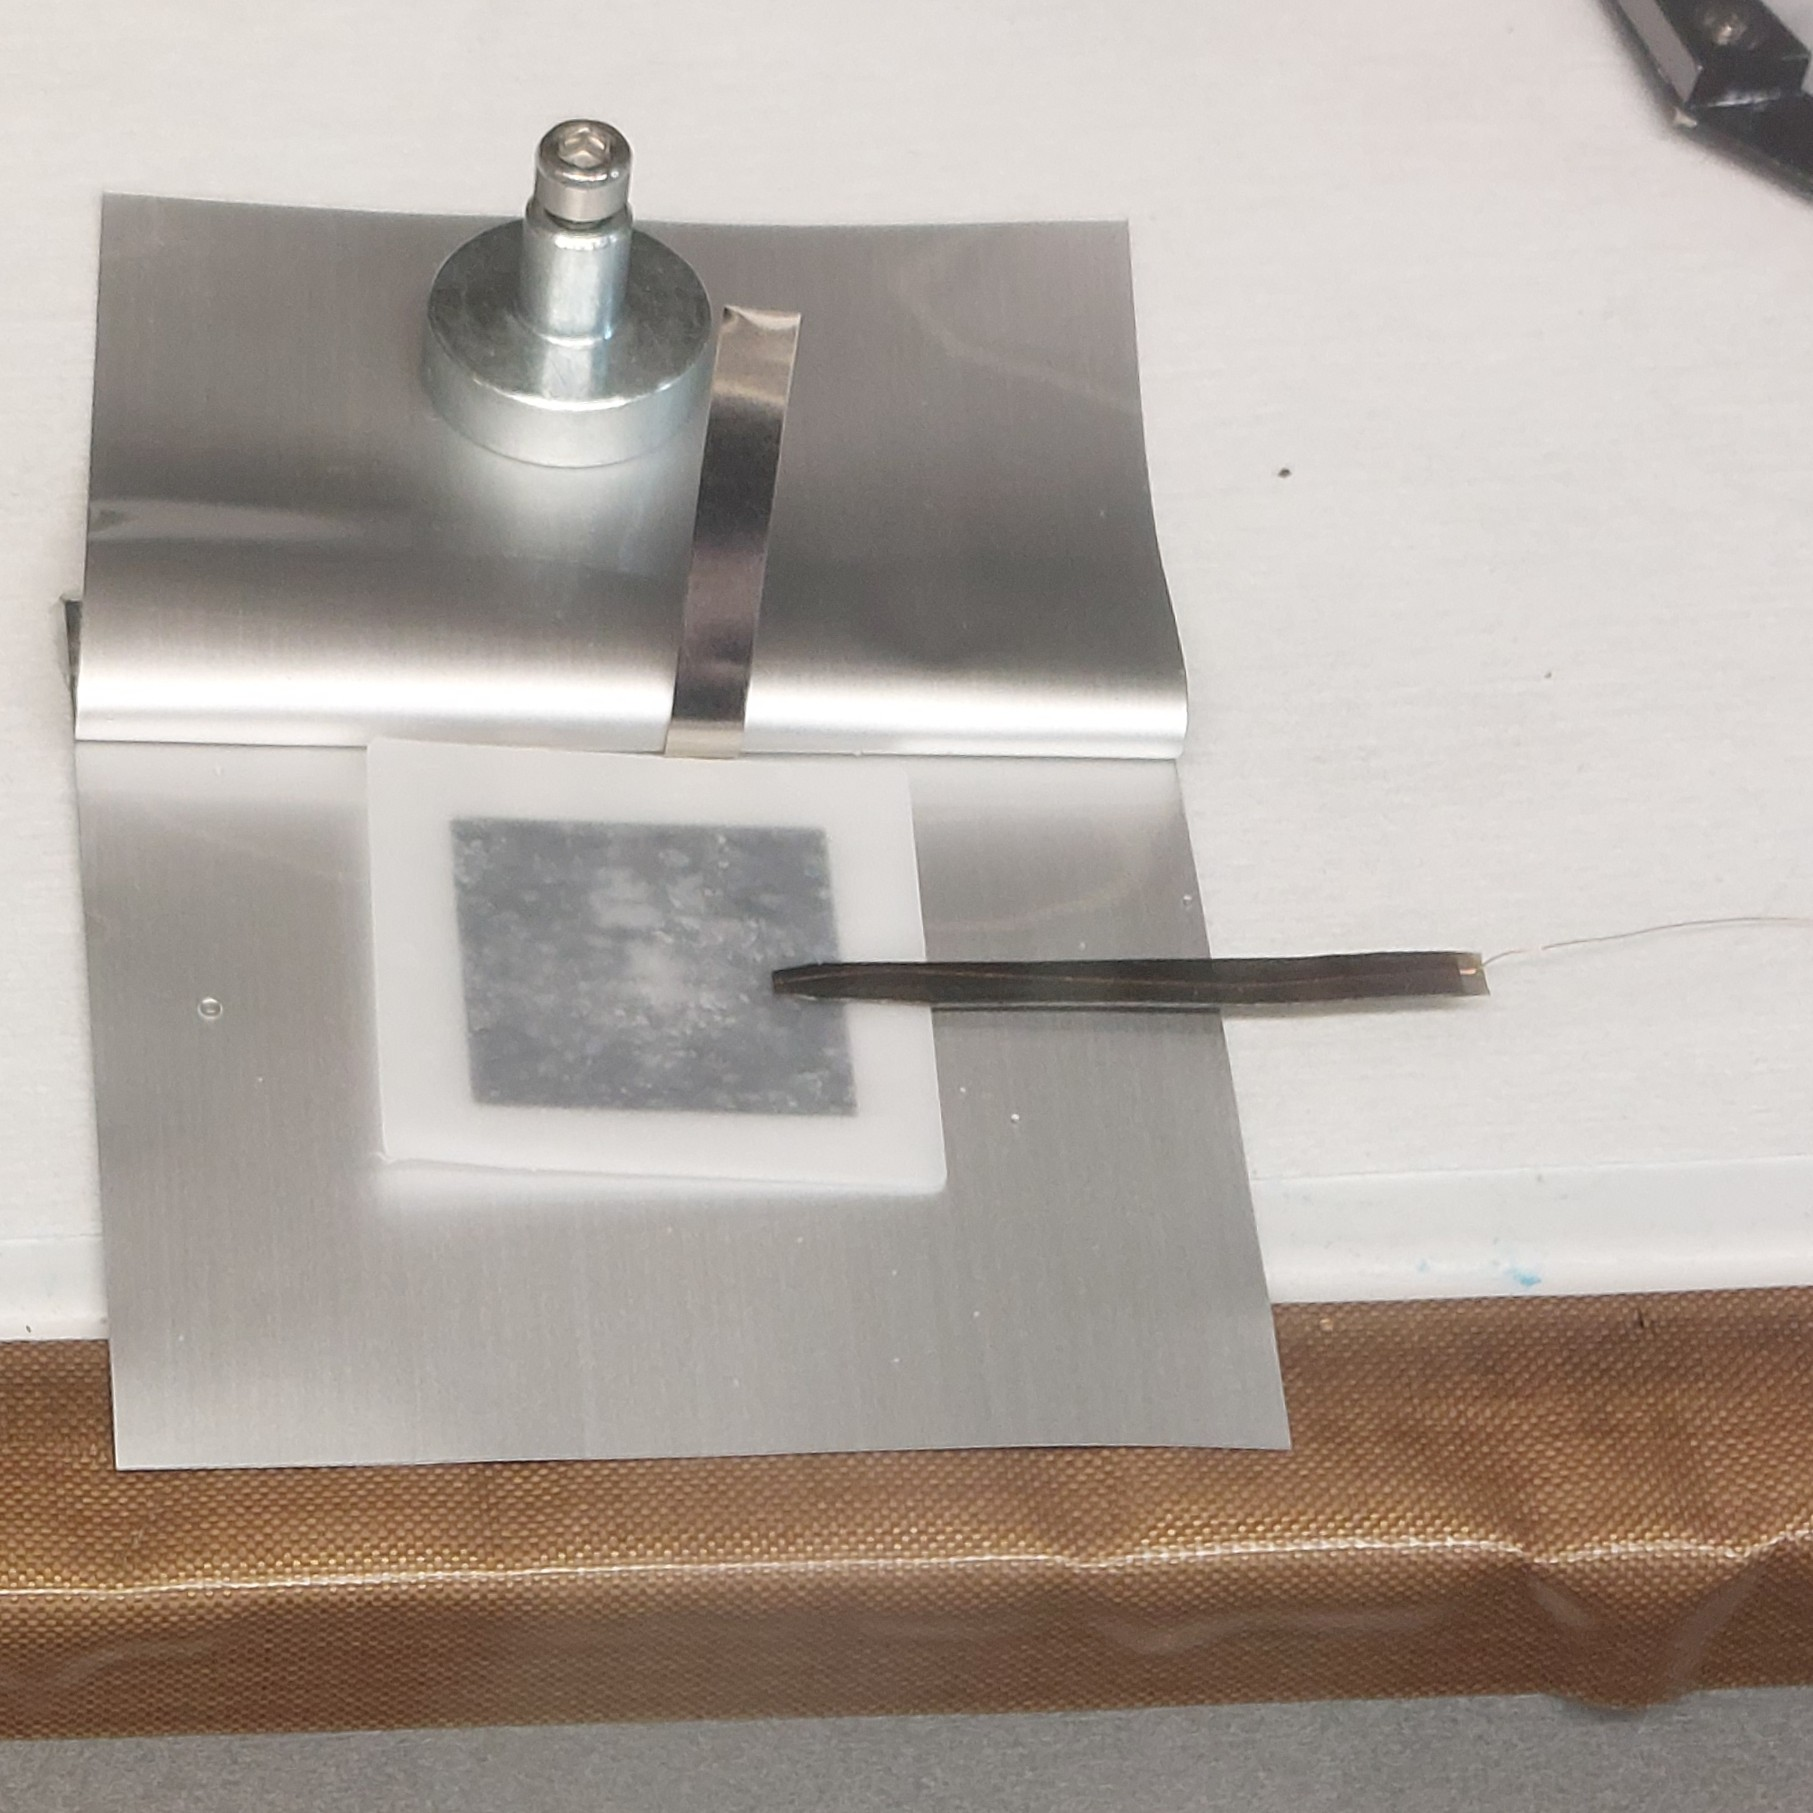
\includegraphics[width=0.4\textwidth]{figures/anodes/graphite_reference_placing.jpg}
    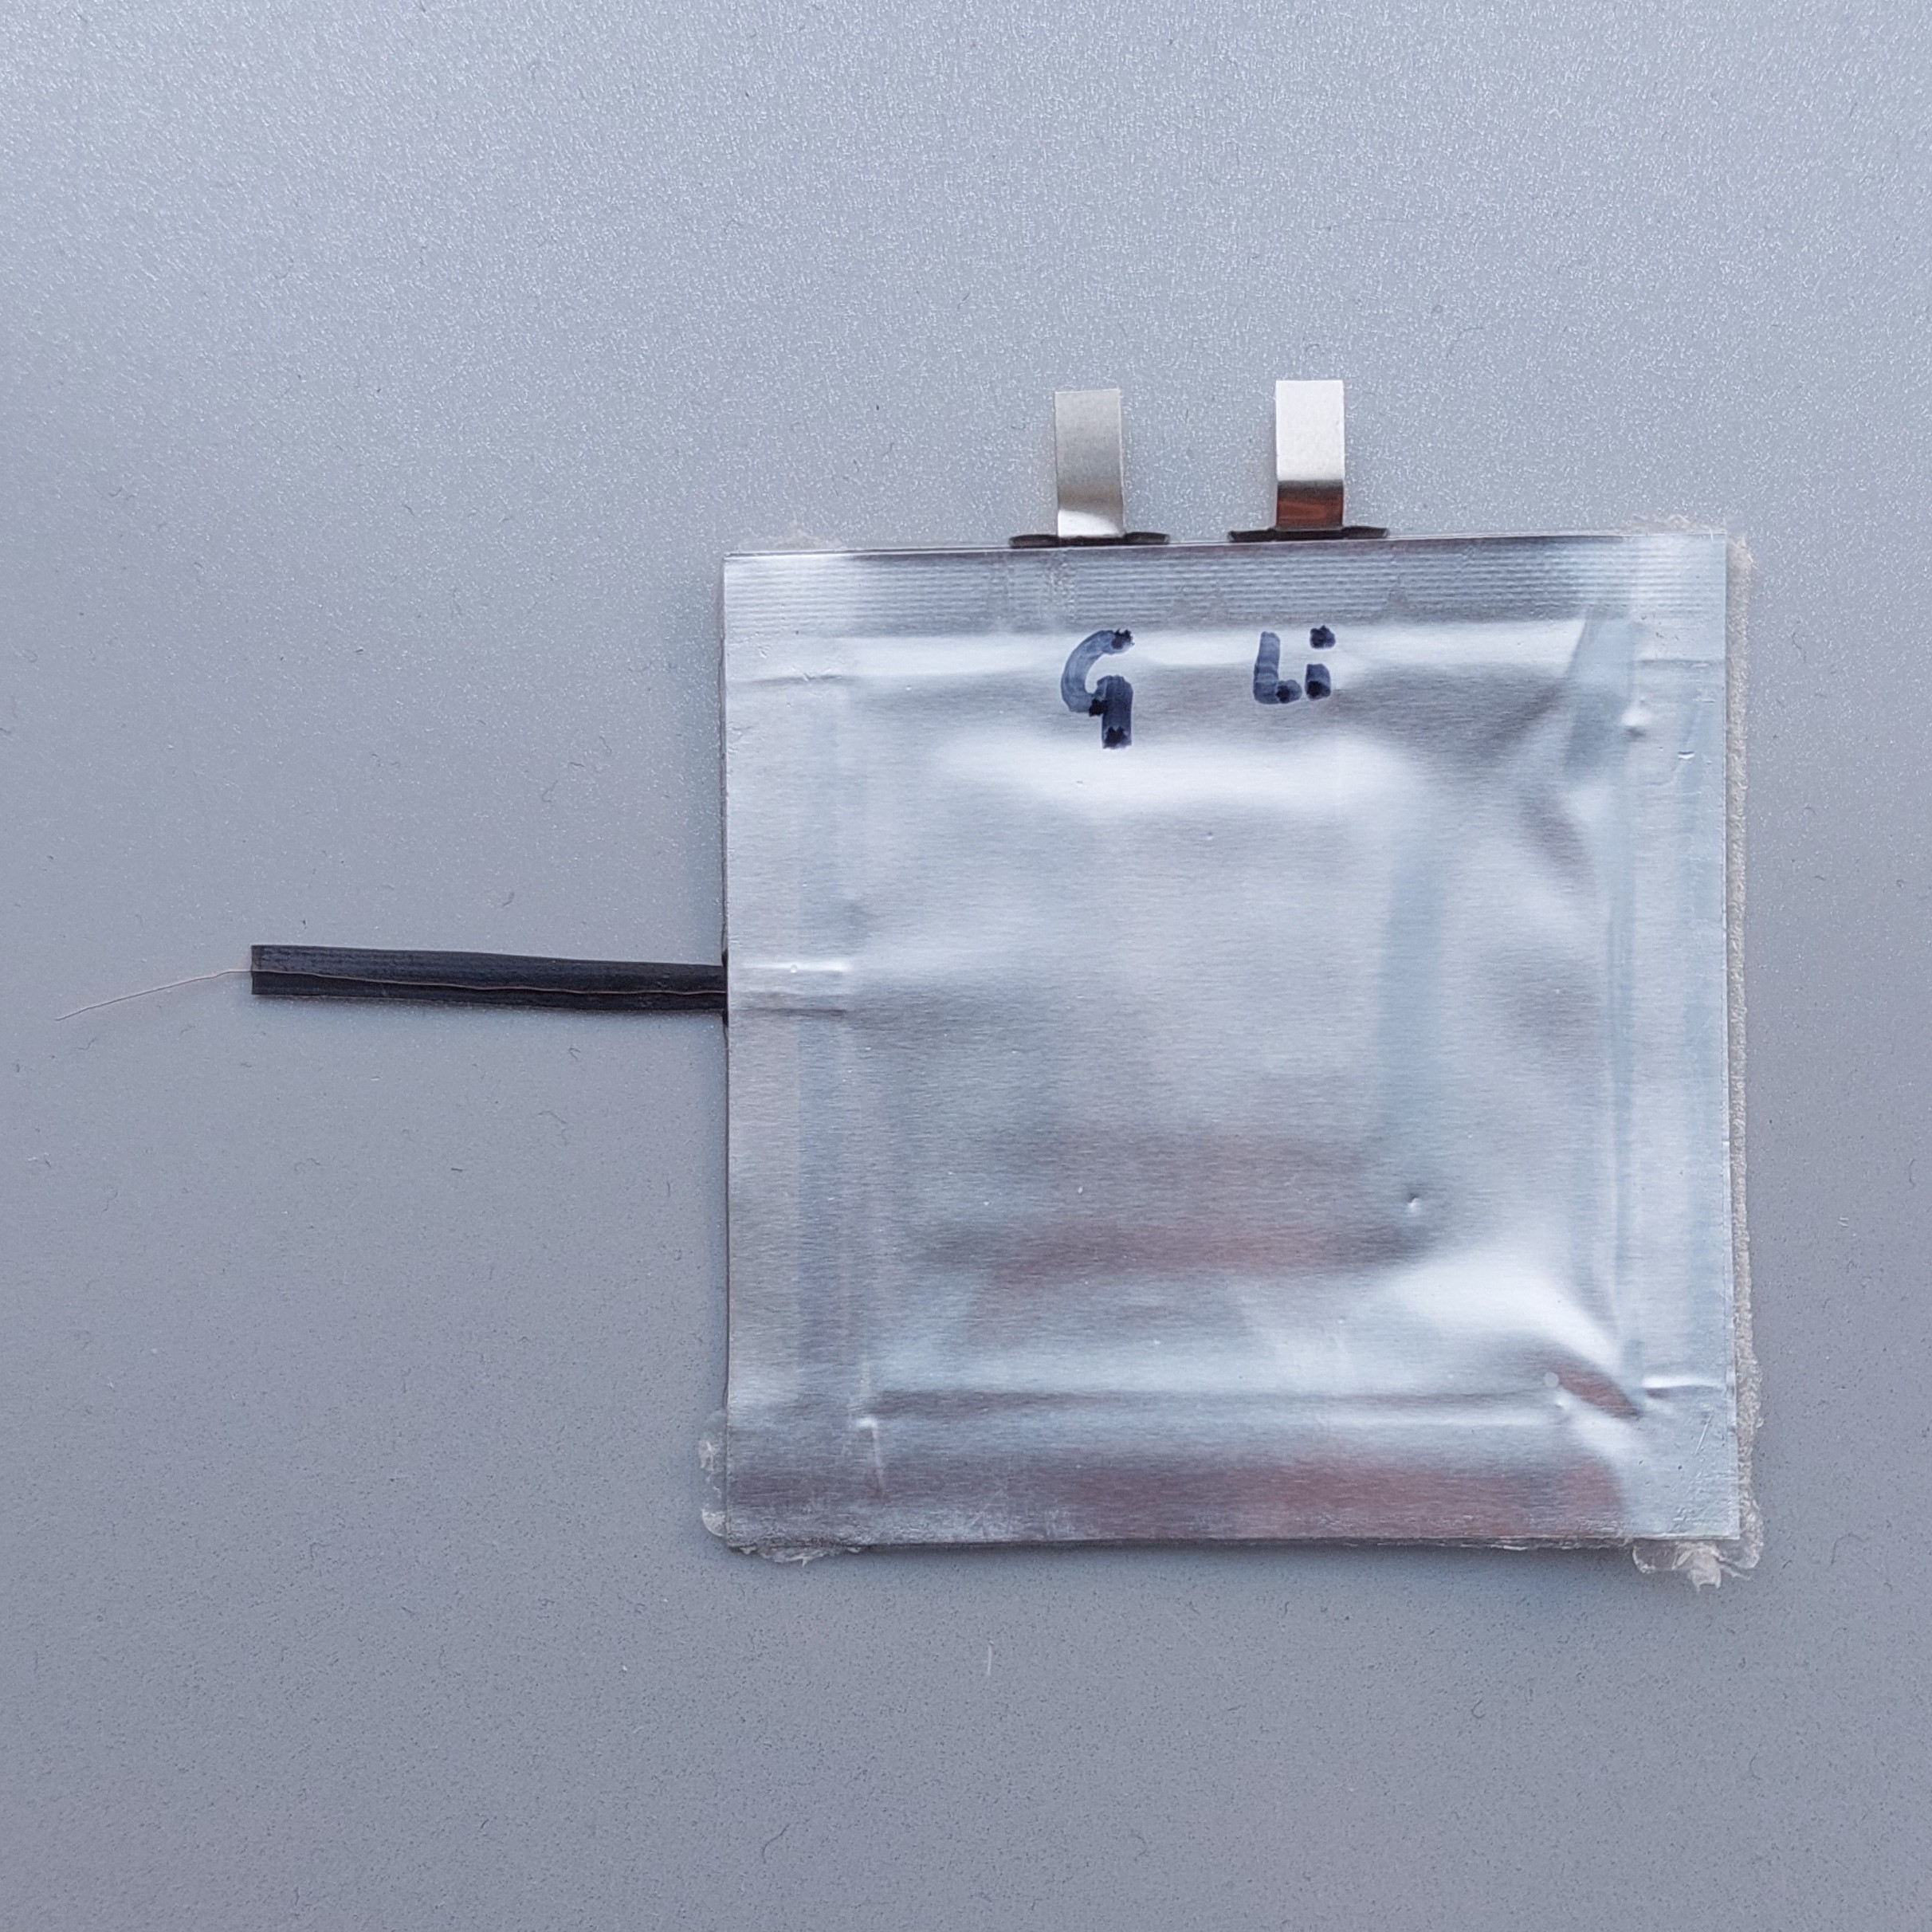
\includegraphics[width=0.4\textwidth]{figures/anodes/graphite_final_pouch_3e.jpg}
\end{figure}

\begin{figure}[H]
    \centering
    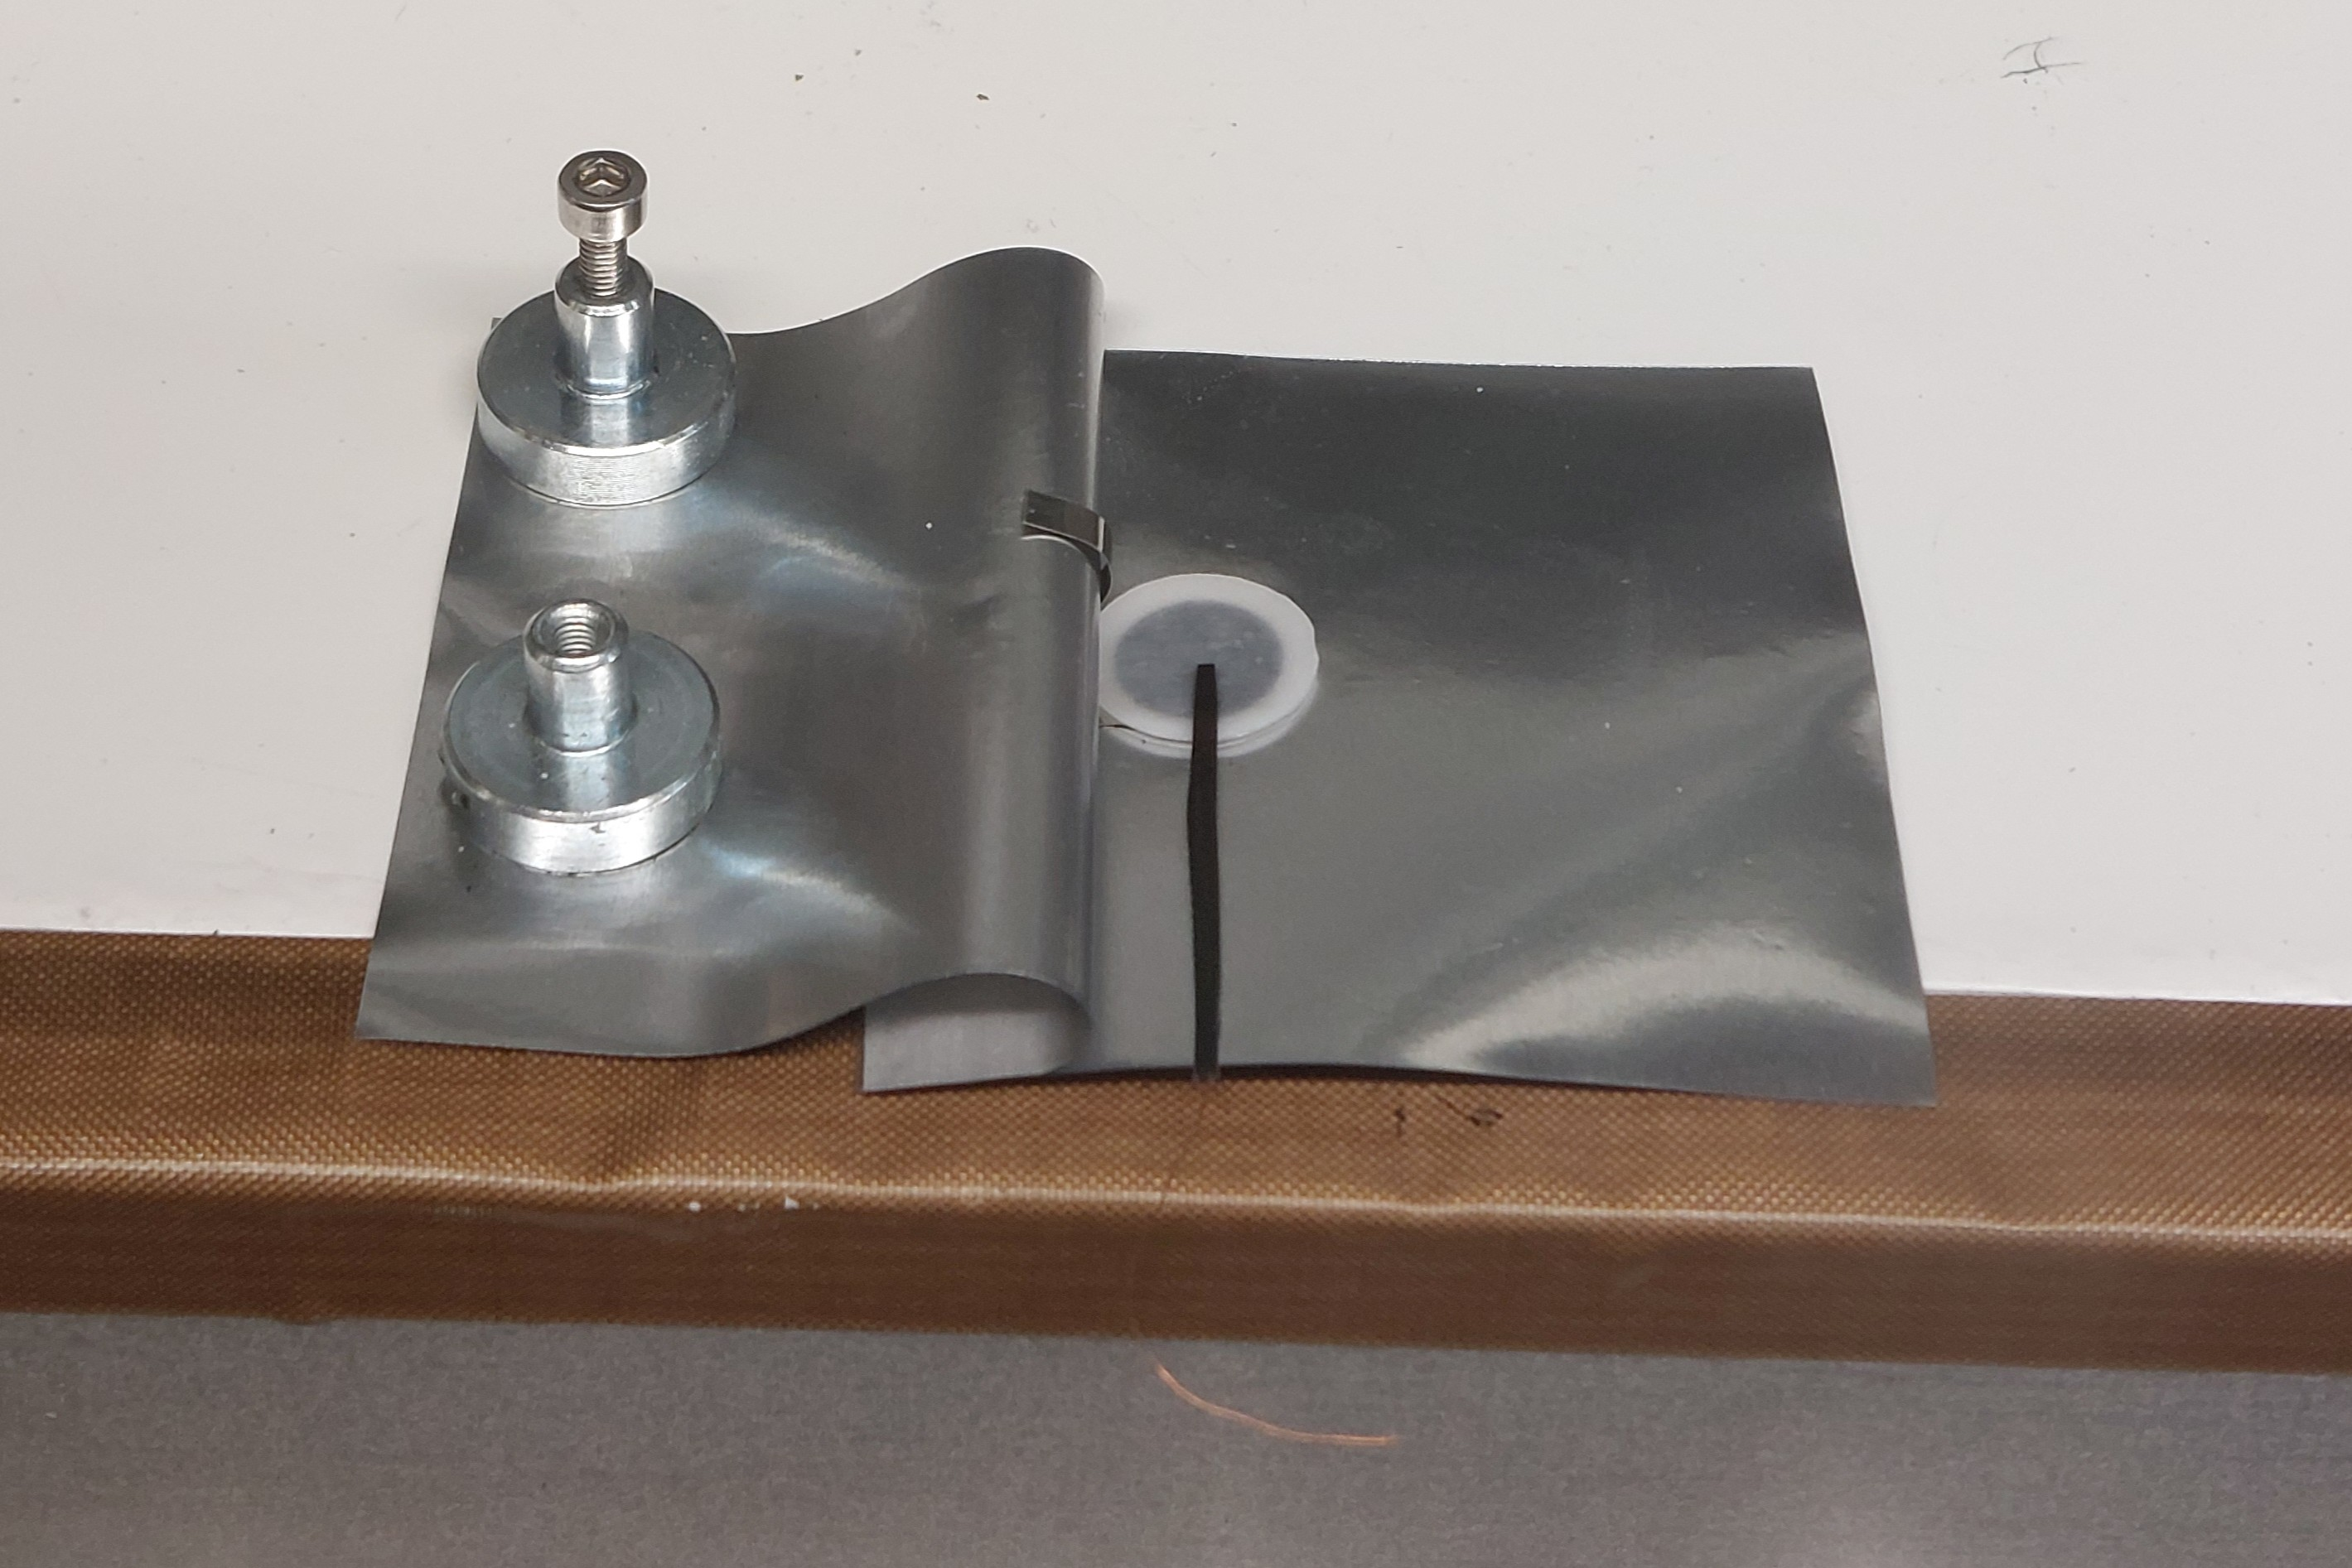
\includegraphics[width=0.5\textwidth]{figures/anodes/SiCN_reference_placing.jpg}
    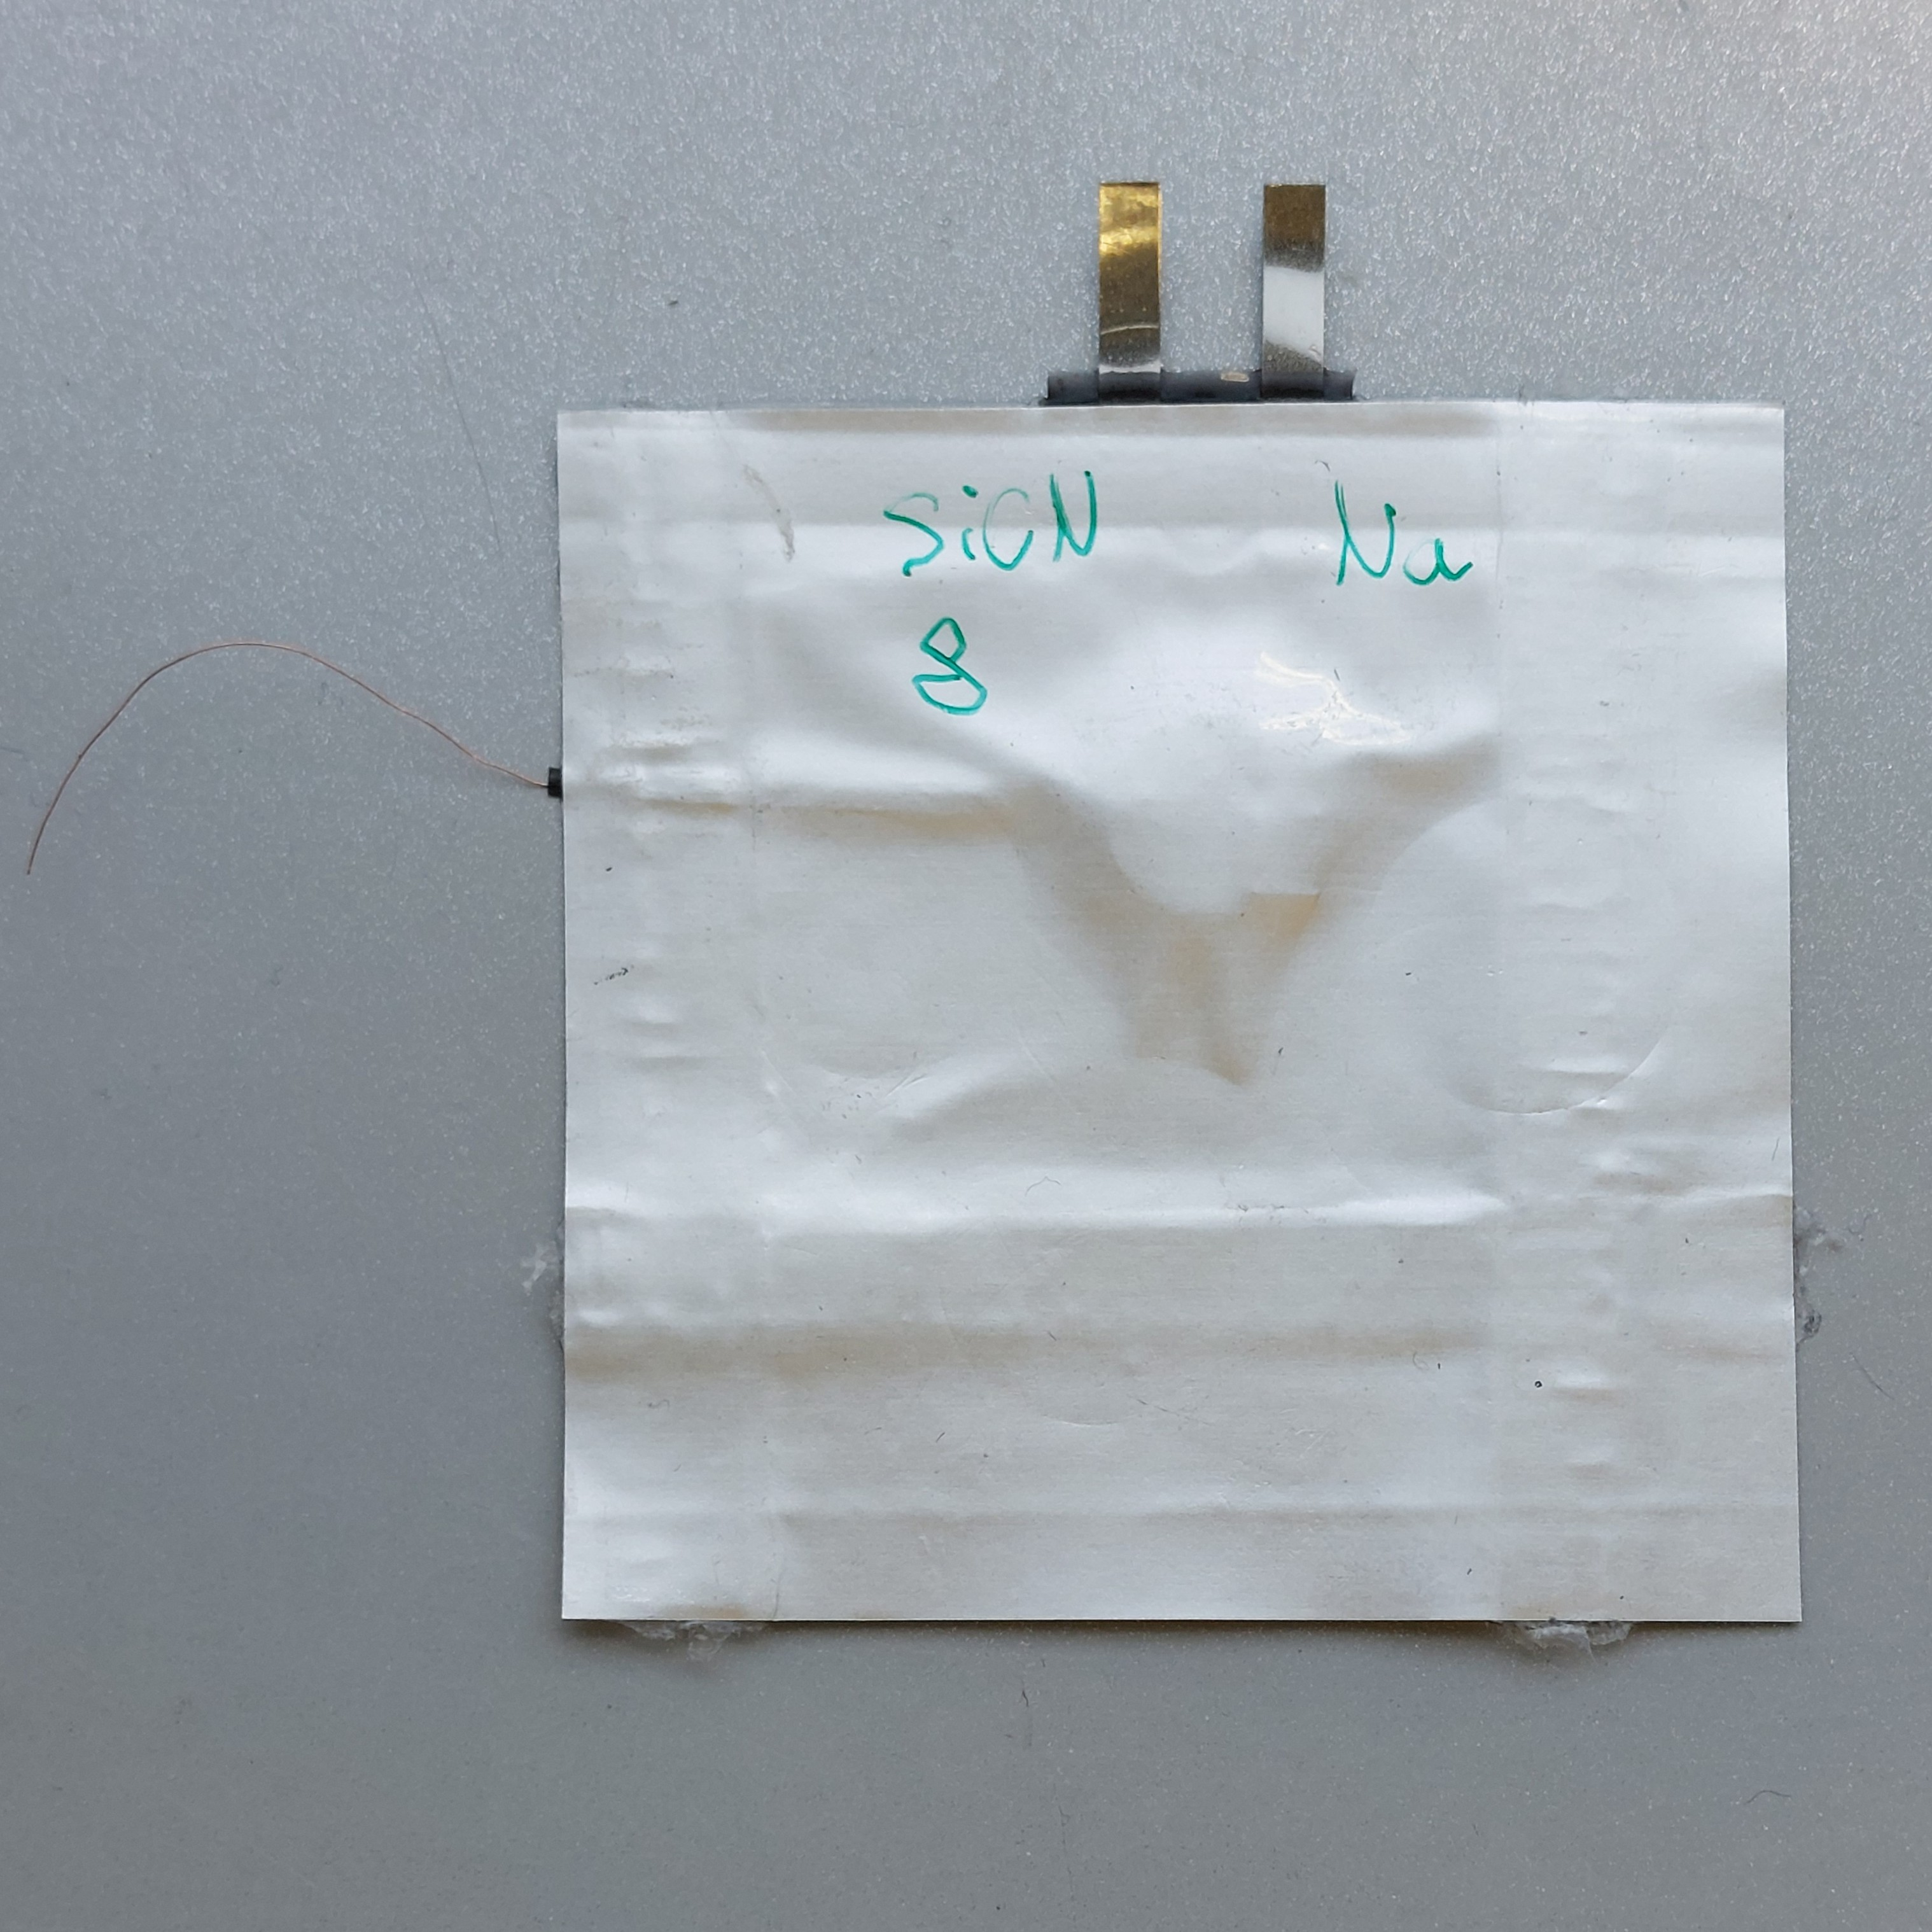
\includegraphics[width=0.4\textwidth]{figures/anodes/SiCN_final_pouch_3e.jpg}
\end{figure}

\section{DEIS setup}
% How the potentiostat is wired to the 3-electrode cell
For this measurement I used the instrumental setup with the automation software (but not online computation of the high frequency impedance) for long acquisition up to 20 hours per half-cycle over multiple cycles. Here the automatino comes in handy again and highlights its importance for material characterization.

\subsection{DEIS measurement parameters for graphite}

\subsection{Applied drift for graphite}

For the graphite I applied galvanostatic cycling with different current rates: C/10, C/5, C/3, 1C, and 2C. They are calculated from the theoretical capacity of 11mAh. The batteries were cycled with an upper voltage limit of 0.8V and 0V against Li/Li+. 

\subsection{Multi-sine excitation for graphite}
I generated a multisine with frequencies from 0.01Hz to 1kHz with 8 points per decade, equal amplitudes across the components and randomized phases (lowest crest factor of then). The multifrequency signal was sampled at 5kHz.
The amplitude of the perturbation was 40mApp except for the experiment at 2C where I used 5mApp. In fact, here the system is at a highly non-linear point and small perturbation are necessary to maintain the output oscillation inside the potetionstat hardware limit. The estimated impedance with this excitation was of poor quality.

\subsection{DEIS measurement parameters for SiCN(O)}
For this application I used the set-up Version 3 as discussed in the experimental section. The main drift consisted only of a galvanostatic reduction and oxidation with potential limitation without any rest or potentiostatic steps, to match the protocol used in a previous publication. 

\subsection{Multi-sine excitation for SiCN(O)}
% Frequenies
% Number of points per decade
% Phase randomization
% Amplitude selection procedure
% Duration of one multisine period
% Was, the multisine the same? I believe not.
The multi-sine was generated with frequency components from 10mHz to 1kHz with 8 points per decades and remove frequencies that produce intermodulation. The amplitude was kept flat and crest factor optimized by random iteration of the phases. After loading the multi-sine on the waveform generator an amplitude of 80mV was set on the instrument. The multi-frequency signal was collected with a sampling frequency of 5kHz.
What was the IRange? It is important to calculate the current amplitude.

\subsection{Applied drift for SiCN(O)}
The current was set to C/20 in respect to the theoretical capacity calculated as ????  in the potential windows of 0V to 2.5V vs Na.

\subsection{DEIS measurement parameters for sodium}

\subsection{Applied drift for sodium}
Galvanostatic

\subsection{Multi-sine excitation for sodium}
I generated a multisine with frequencies from 0.01Hz to 25kHz with 8 points per decade, equal amplitudes across the components and randomized phases (lowest crest factor of then). The multifrequency signal was sampled at 100kHz.


\subsection{Impedance estimation}
% DMFA
% Bandwidth 0.1 Hz
% Choice of n = 8
% Block size
% Removal of DC trends
For all the measurement the time-varying impedance is estimated totally off-line through Dynamic Multi-Frequency Analysis using a Symmetric Fermi-Dirac filter with 0.01Hz of bandwidth and order $n=8$. In both current and voltage signal I removed a linear baseline.

\section{Results and disucssions}

\subsection{Results of graphite}
% Qualitative evaluation of the impedance at all c-rates.
% Comment on the change of the low frequency part in the plateaus as for LTP
% Comment that this information disappears at 1C, it is already quite fast dynamics for this system.
% Comment the reduction of impedance temporary.
% Comment the asymmetry between charge and dischare
% Comment the increase of impedance with the current density
Before performing the DEIS experiment, I perormed formation and 1C cyclation with limitation on maximum charge equal to the nominal capacity.

The result of dynamic impedance at C/5 are shown in \ref{fig:graphite_C5}.
\begin{figure}[H]
    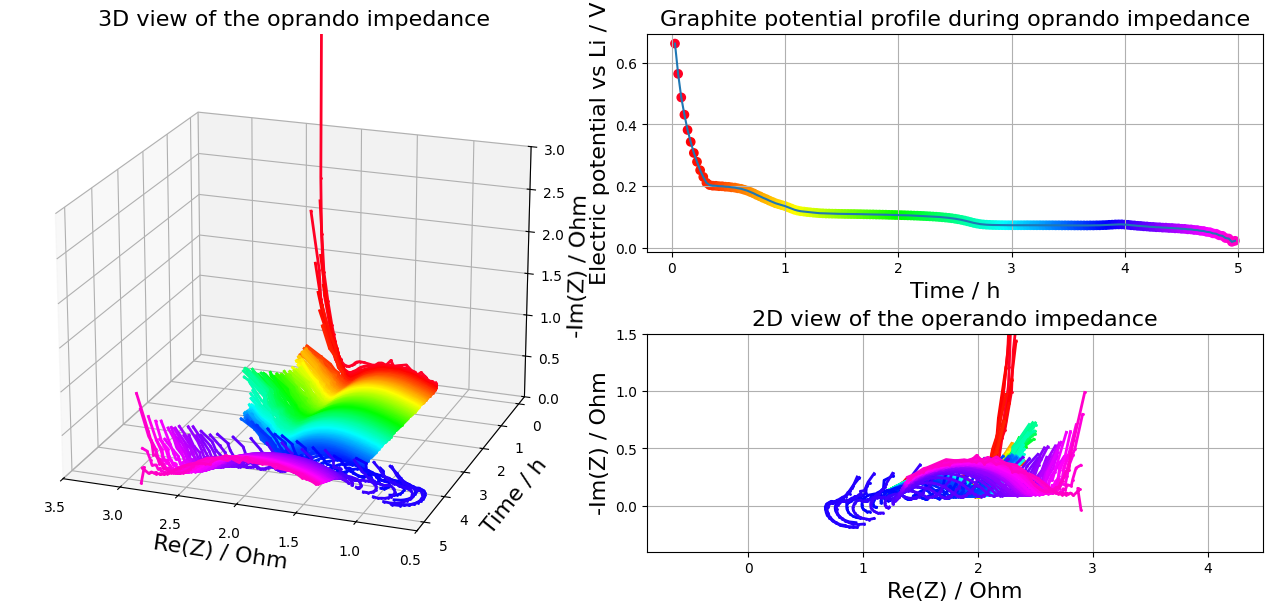
\includegraphics[width = 0.5\textwidth]{figures/anodes/graphite_reduction_C5.png}
    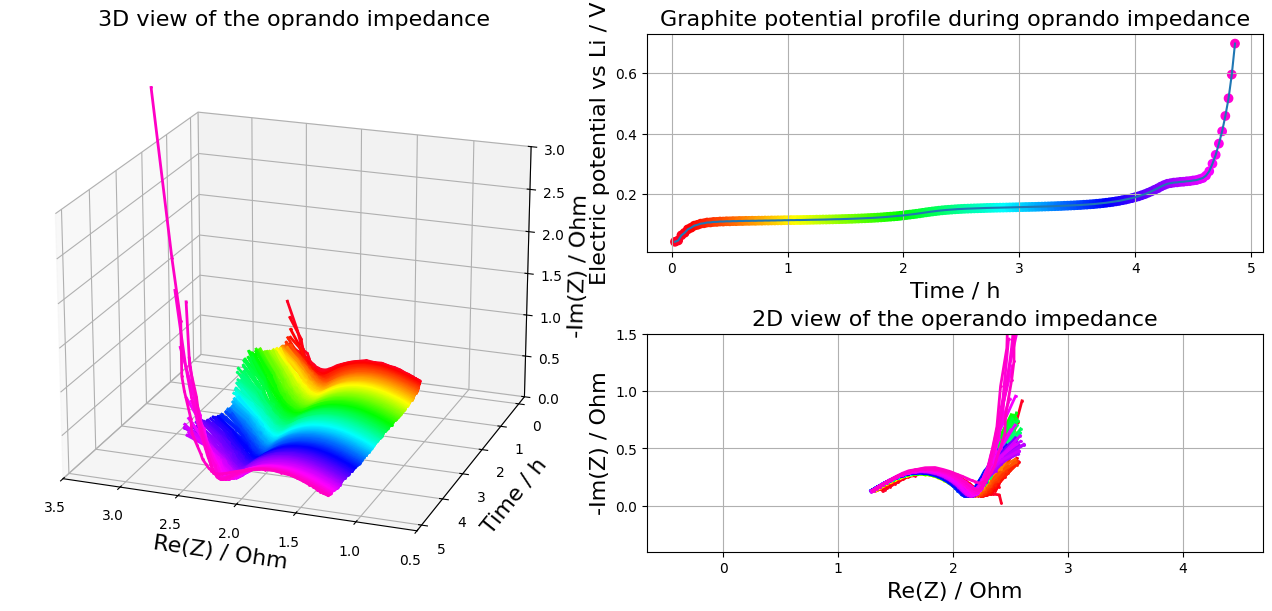
\includegraphics[width = 0.5\textwidth]{figures/anodes/graphite_oxidation_C5.png}
    \caption{Full cycle of galvanostatic C/5 with DEIS. Removed first spectra and 10mHz frequency point.}
    \label{fig:graphite_C5}
\end{figure}
From a qualitative evaluation we observe that the diffusional tail change in proximity of phase changes (the colours help to identify the match between the voltage and the impedance) as observed also for Lithium Titianium Phosphate. 
This behaviour is present in both fro cathodic and anodic currents, signaling a processes intrinsic of the graphite electrode. 
I suspect that is the change in volume during intercalation that affects the tortuosity of lithium ion in the porous electrode.
Though, for cathodic currents, towards the end of the intercalation a sudden change of the impedance magnetude appears where the system become "faster" in the sense of characteristic time constant.
Figure \ref{fig:graphite_C5} shows an enlargment of the dataset in the region where this phenomena occours and the left side is the plot of the ipedance at its lower value to appreciate the shape. Unfortuanlty, when the impedance get smaller fot the same amplitude of the escitation the response gets a lower signal to noise ration which afects the precision of the impedance estimation.
\begin{figure}[H]
    \centering
    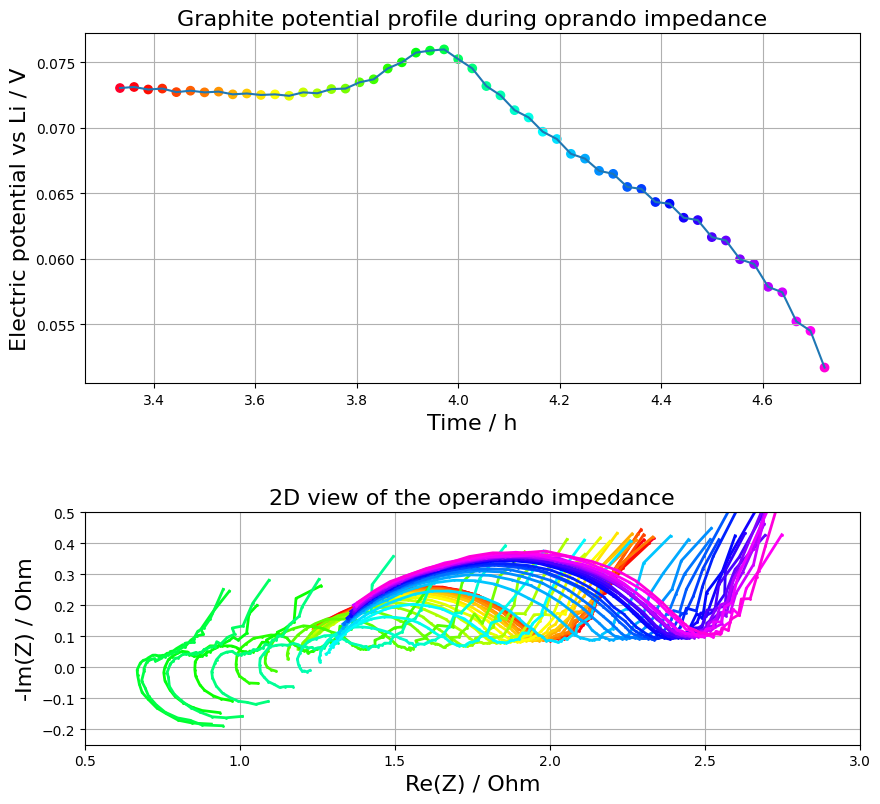
\includegraphics[width = 0.4\textwidth]{figures/anodes/graphite_feature_zoom.png}
    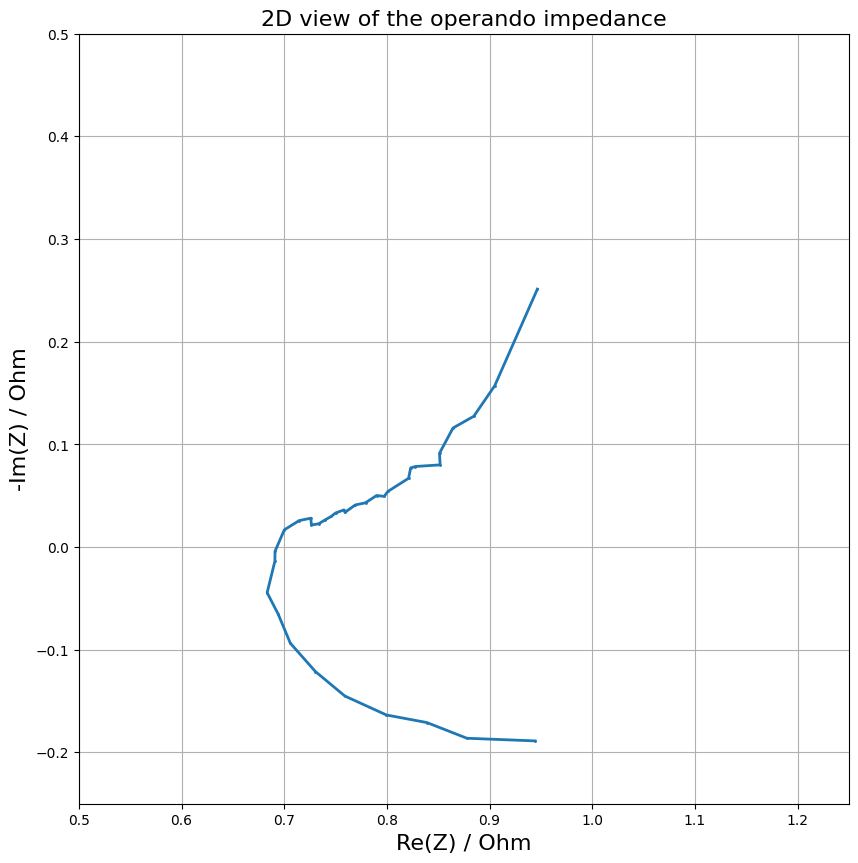
\includegraphics[width = 0.3\textwidth]{figures/anodes/graphite_single_impedance_feature.png}
    \caption{Zoom in at the feature at C/5}
    \label{fig:graphite_feature_zoom}
\end{figure}
It is interesting to notice an increase of the voltage in corrispondance of the reduction of surface impedance.
Smaller overvoltage is in accordance with the lower charge transfer. 
If we add the fact that the processes doesn't appear with anodic currents, I suspect that it could be connect with lithium electrodeposition in local area where the electrode potential, being not uniform thought the electrode surface and thickness, is negative.

When performing the DEIS experiment at 1C current density, reported in Figure \ref{fig:graphite_1C} the sudden process is not observed, but also the characeristics plateau of the electrode potential are not distinguiscible and the diffusional tail of the impedance doesn't seem affected. 
\begin{figure}[H]
    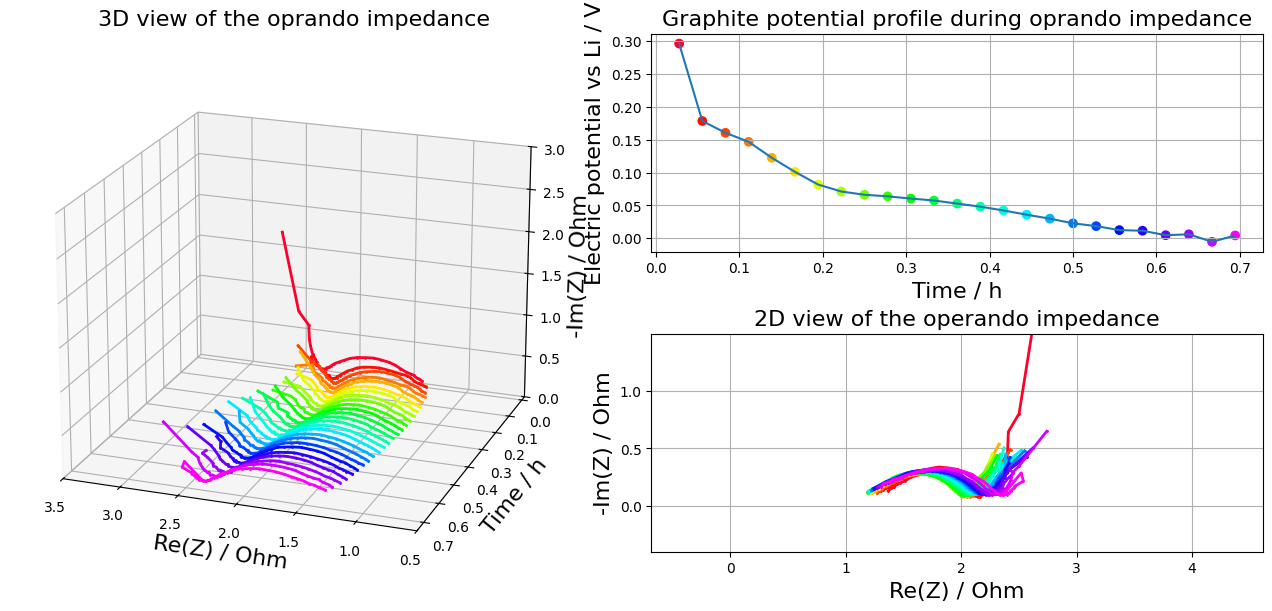
\includegraphics[width = 0.5\textwidth]{figures/anodes/graphite_reduction_1C.png}
    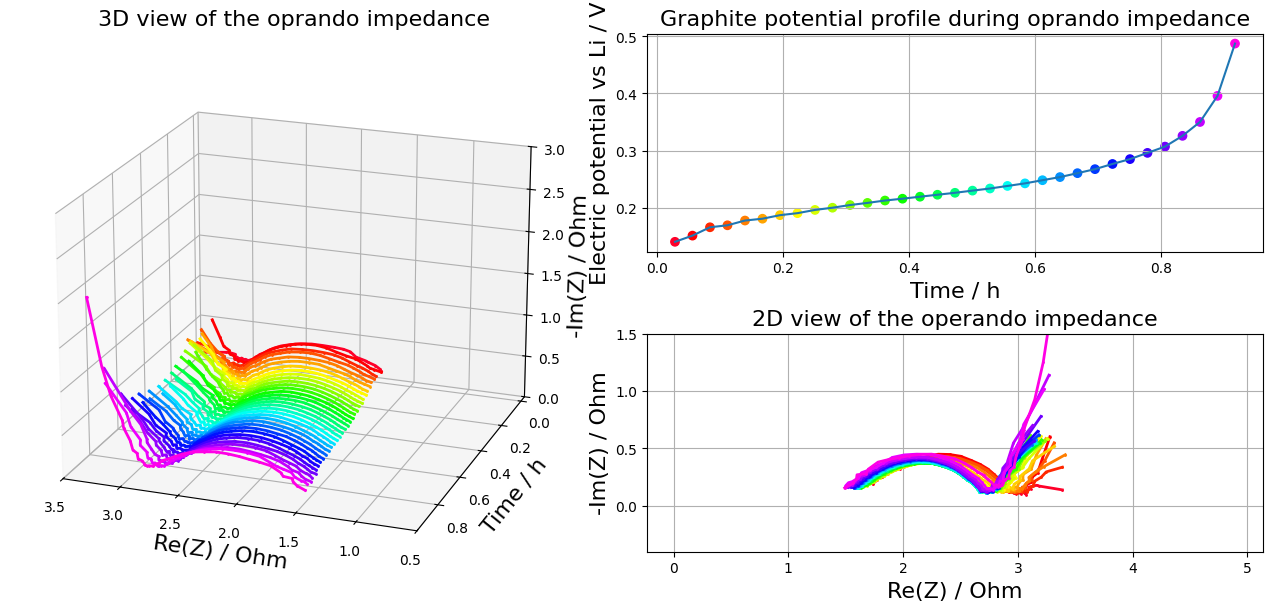
\includegraphics[width = 0.5\textwidth]{figures/anodes/graphite_oxidation_1C.png}
    \caption{Full cycle of galvanostatic 1C with DEIS}
    \label{fig:graphite_1C}
\end{figure}
At high current rates, the overvoltage is so high that the third intercalation plateau is not reached and around 70\% of the nominal capacity is stored.
This explains the missing processes compared to the case at C/5. 

The measurement of impedance in non-stationary conditions highlights also the importance of the c-rate, hence the concentration profile at the interface, in the process kinetics. Figure \ref{fig:graphite impedance comparison} shows comparison of the impedance at 50\% state of charge for different c-rates and both directions of the current.
\begin{figure}[H]
    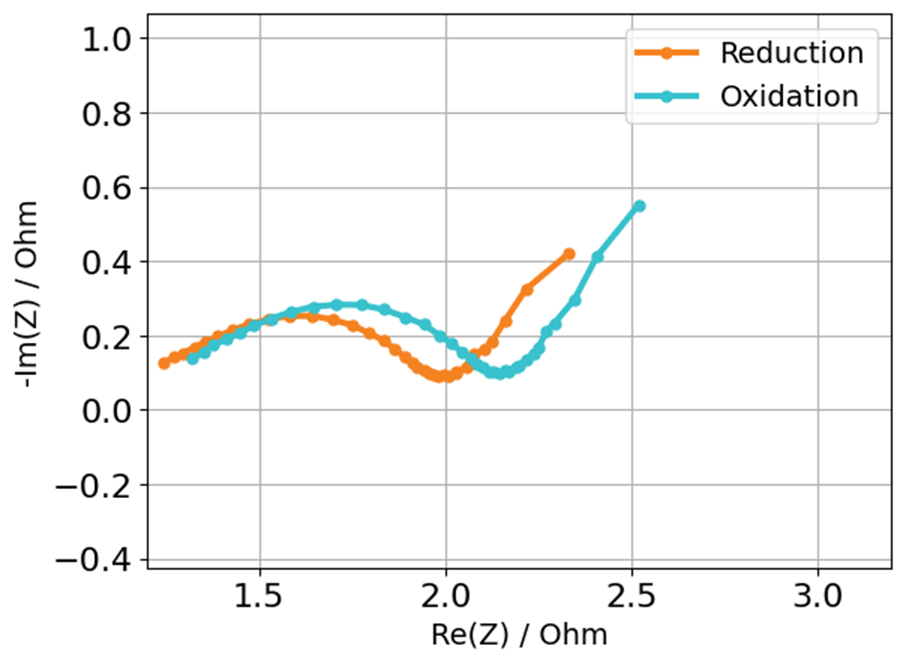
\includegraphics[width = 0.3\textwidth]{figures/anodes/image7.png}
    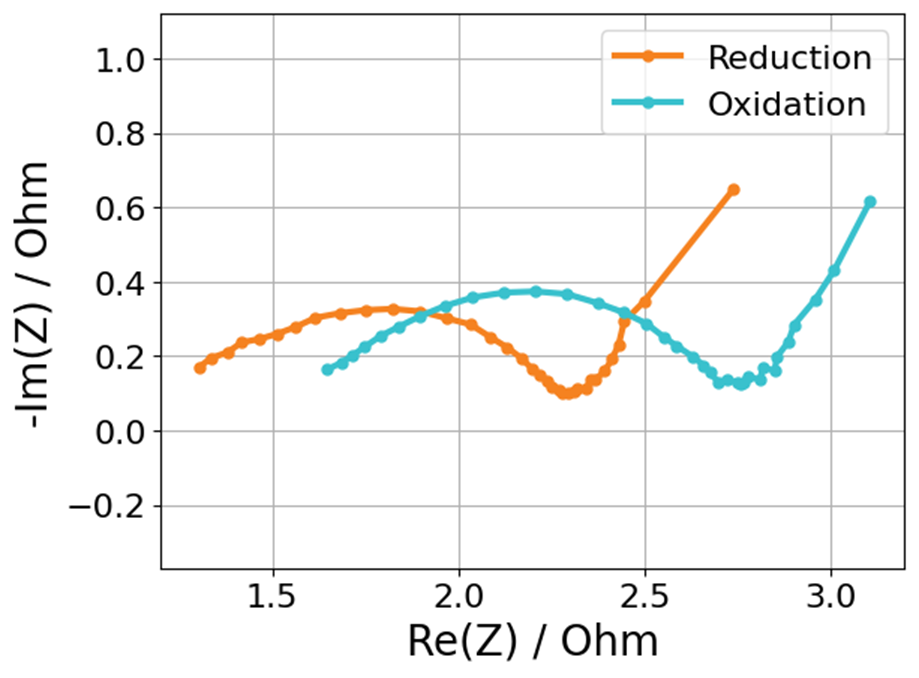
\includegraphics[width = 0.3\textwidth]{figures/anodes/image8.png}
    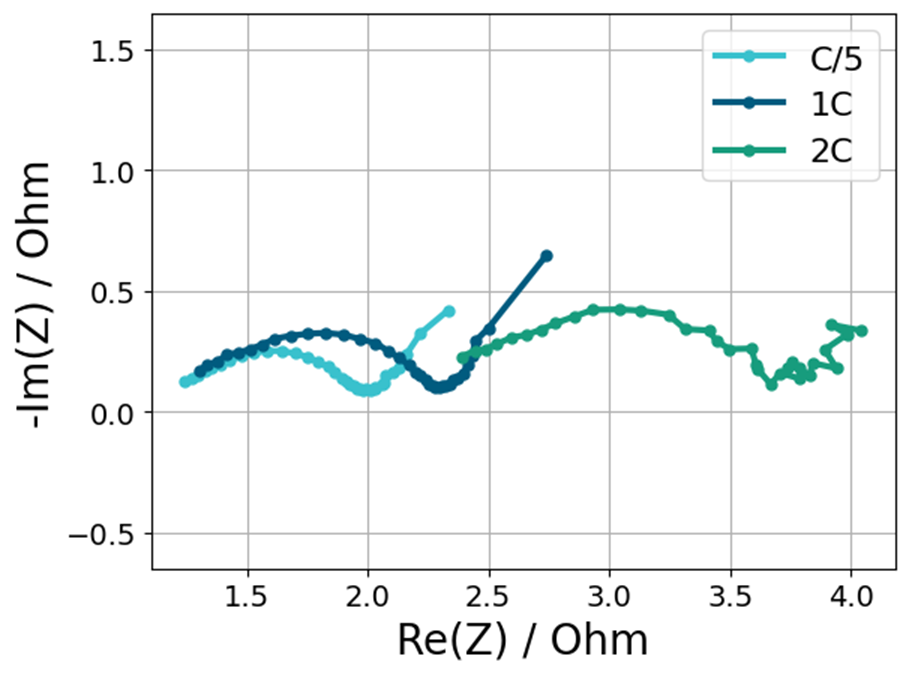
\includegraphics[width = 0.3\textwidth]{figures/anodes/image9.png}
    \caption{Comparison of impedances at different states. From left to right: impedance at}
    \label{fig:graphite impedance comparison}
\end{figure}
The asimmetry of impedance for cathodic and anodic currents is observed here as in for the LTP electrode, but here there is also the information on the effect of the current density which produces an increase of the high frequency resistance and charge transfer semicircle. The increase become greater when jumping from 1C to 2C current rates.
This could also be due to skin effect [cite King et al. 2025 J. Electrochemical Soc.].
At high current density 2C the impedance is very noisy because of the high non-linearity introduced by the excitation. 
Trying to reduce the amplitude of the excitation doesn't help much beacuse then a low sigal to nose ratio impares the precision anyway. 
This is especially critical for the low frequency that are strongly superimposed to the drift at high c-rate cycles.

Unfortunalty the failed reproduction of the reference electrode made impossible to verify this behaviour for different electrode hystory or full cells with NCM cathods (despite dozens of attempts).

\subsection{Results of SiCN(O)}
% Show results for the two cell both in formation and second cycle
% Point out the importance of SEI formation
% Show that it is reproducible
% Comment that the there is the problem of fixed amplitude and decrease in impedance that ruins the quality
% Comment that we see the same temporal reduction of impedance toward the end of the half-cycle.

The experiments of this electrodes were performed from fresh so the first cycle of DEIS galvanostatic cycling shows also the SEI formation process, as reported in Figure \ref{fig:SiCN cell 36 first cycle}
\begin{figure}[H]
    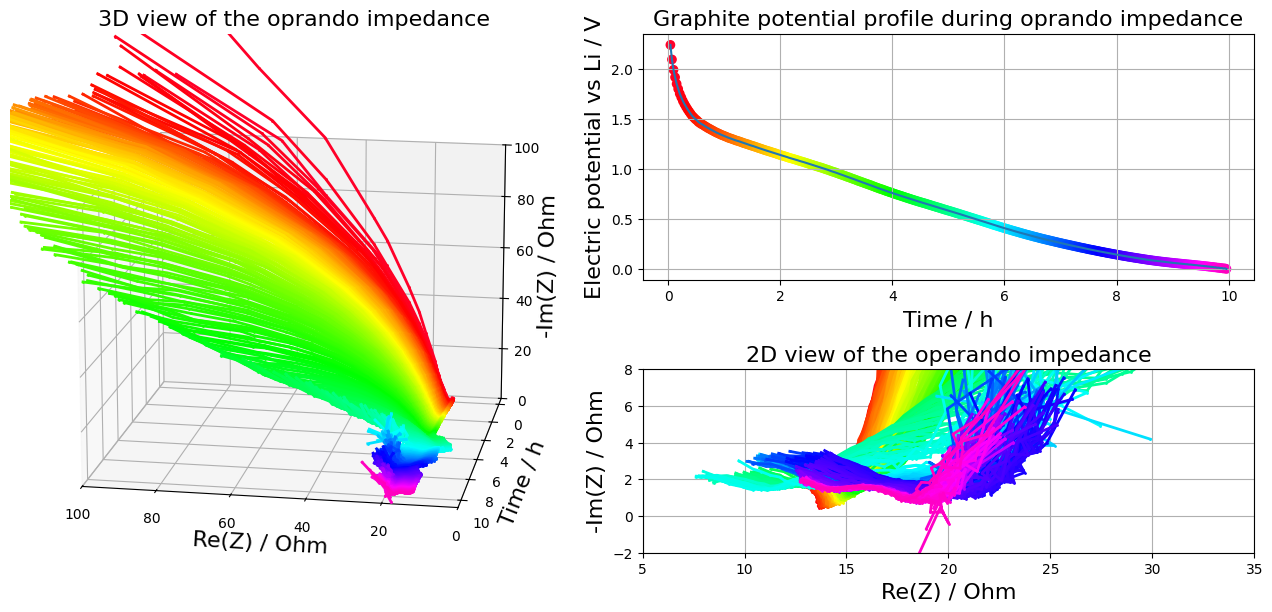
\includegraphics[width = 0.5\textwidth]{figures/anodes/SiCN_pouch36_1.png}
    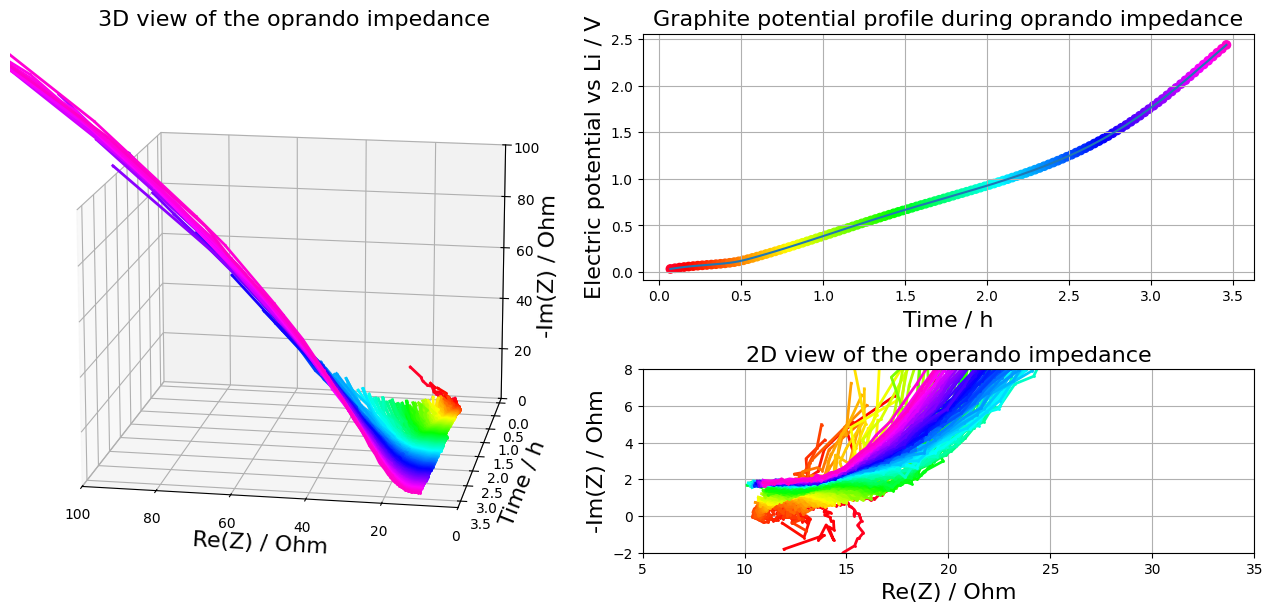
\includegraphics[width = 0.5\textwidth]{figures/anodes/SiCN_pouch36_2.png}
    \caption{Full first cycle of galvanostatic C10 SiCN with DEIS}
    \label{fig:SiCN cell 36 first cycle}
\end{figure}
During the formation step, between 1V and 0.5V the impedance is big and then shrinks. The effect of the formation is clear looking at the impednace for anodic chrono-potentiometry.
A look at the sequent cycle conferm the separaton between formation impedance and electrode impedance and shows that the real capacity is less than half the nominal capacity, used also to calculate the current applied in the experiment.
\begin{figure}[H]
    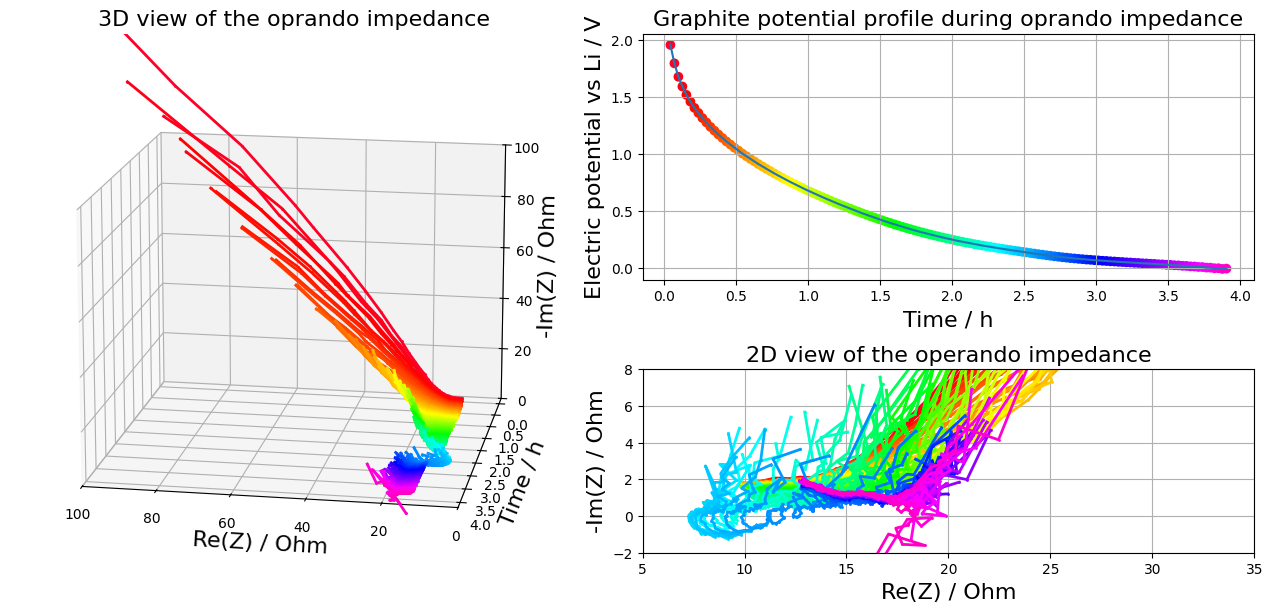
\includegraphics[width = 0.5\textwidth]{figures/anodes/SiCN_pouch36_3.png}
    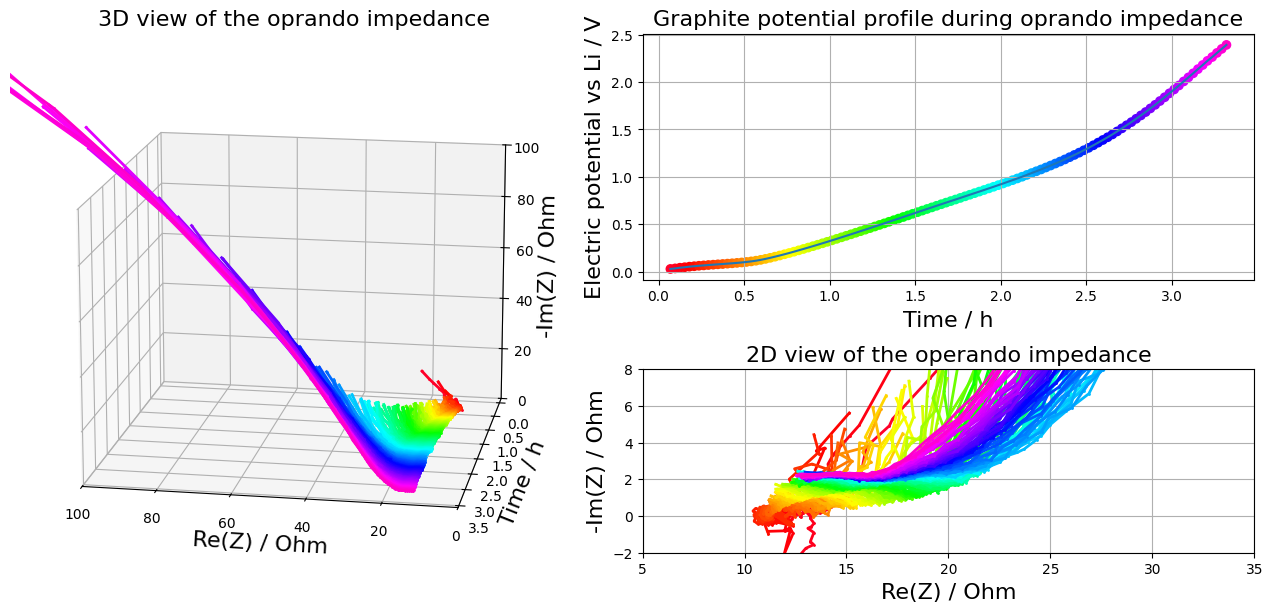
\includegraphics[width = 0.5\textwidth]{figures/anodes/SiCN_pouch36_4.png}
    \caption{Full second cycle of galvanostatic C10 SiCN with DEIS}
    \label{fig:SiCN cell 36 second cycle}
\end{figure}
Looking at Figure \ref{fig:SiCN cell 36 second cycle} one sees again the sudden decrese of the impedance as seen above for graphite.
Figure \ref{fig:SiCN_feature_zoom} shows an enlargment of that part of the dataset.
\begin{figure}[H]
    \centering
    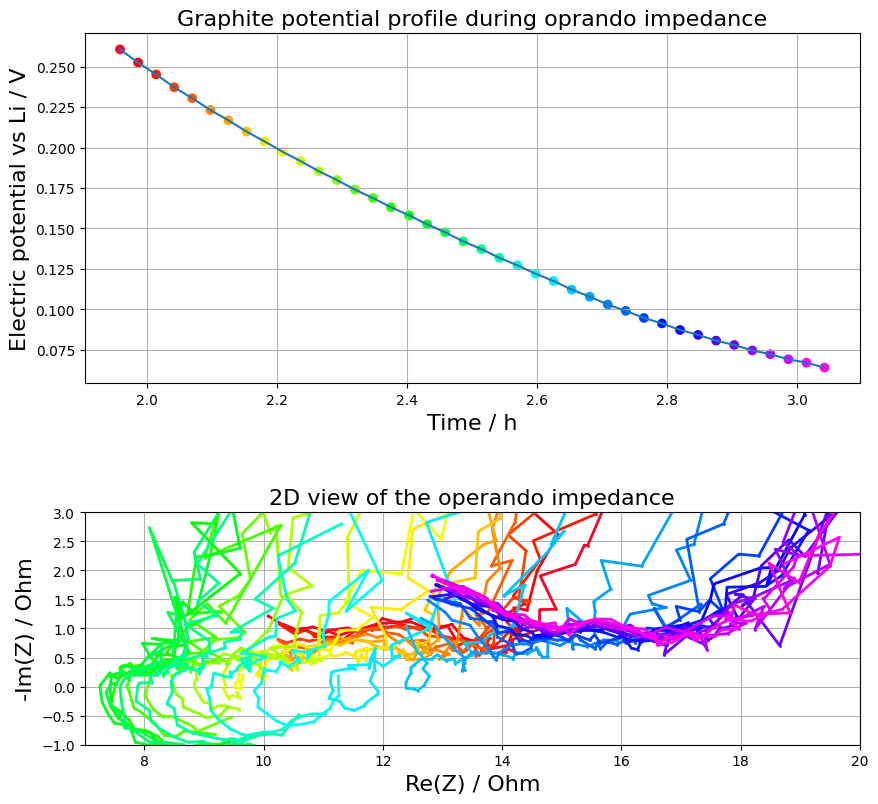
\includegraphics[width = 0.4\textwidth]{figures/anodes/SiCN_feature_zoom.png}
    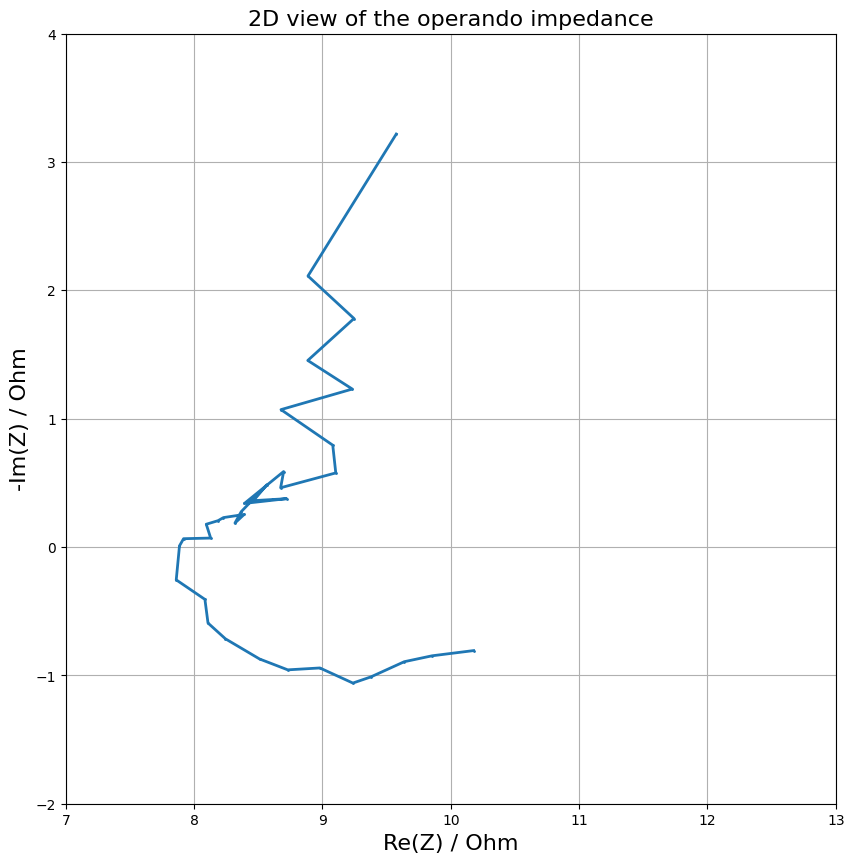
\includegraphics[width = 0.3\textwidth]{figures/anodes/SiCN_single_impedance_feature.png}
    \caption{Zoom in at the feature for SiCN}
    \label{fig:SiCN_feature_zoom}
\end{figure}
The behaviour is analogous for the case of graphite, but no 
The right plot in Figure \ref{fig:SiCN_feature_zoom} shows the same shape seen before for the graphite (Figure \ref{fig:graphite_feature_zoom}), making me thinking that this is more than a coincidence. 
In this case, it would be metallic Sodium to deposit in the pores of Silicon Carbonitrate and could support the theory. 
Contrary to the other case, here we do not see an increase of electro potential associated with the rduction in impedance.

In any case sodium is certainly plating on the surface of the electrode as identified in post mortem inspection (Figure \ref{fig:SiCN post mortem}).
\begin{figure}[H]
    \centering
    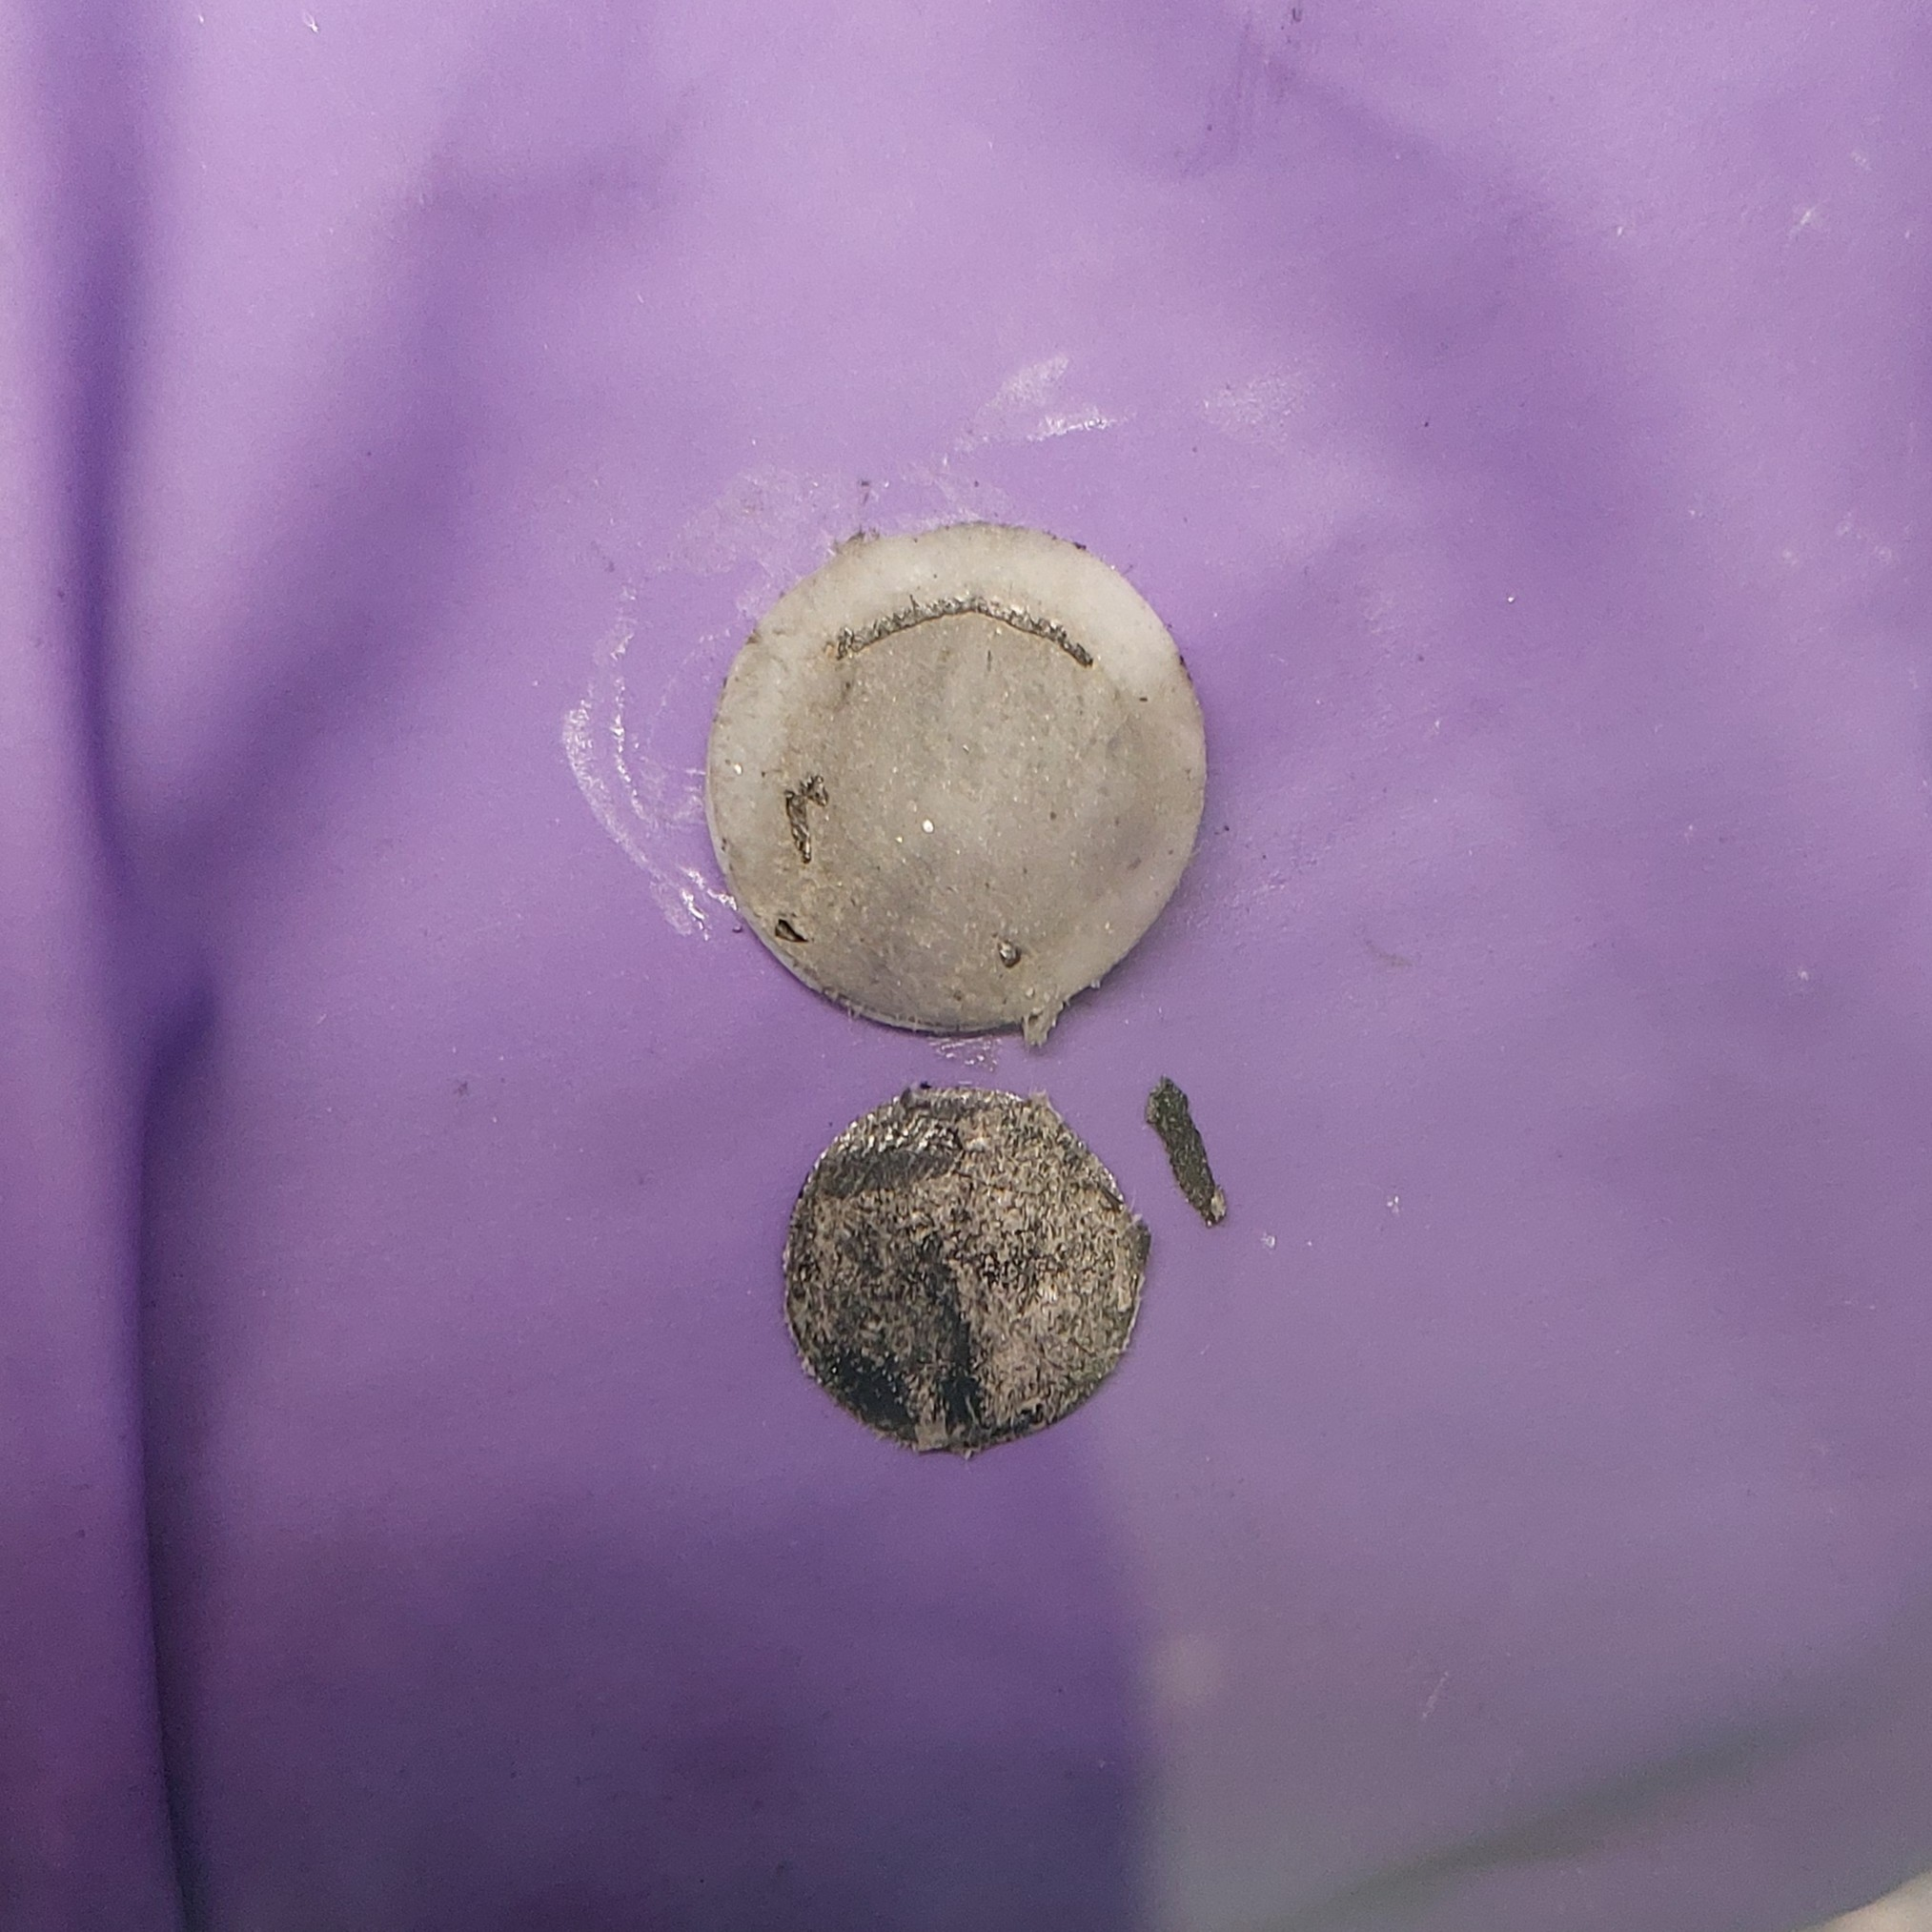
\includegraphics[width = 0.4\textwidth]{figures/anodes/SiCN_post_mortem.jpg}
    \caption{Photo of a SiCN electrode with clear sign of metallic Sodium electrodeposite}
    \label{fig:SiCN post mortem}
\end{figure}

Unfortunatly repeating the experiment led to different results as shown in Figure \ref{fig:SiCN cell 39 first cycle}.
\begin{figure}[H]
    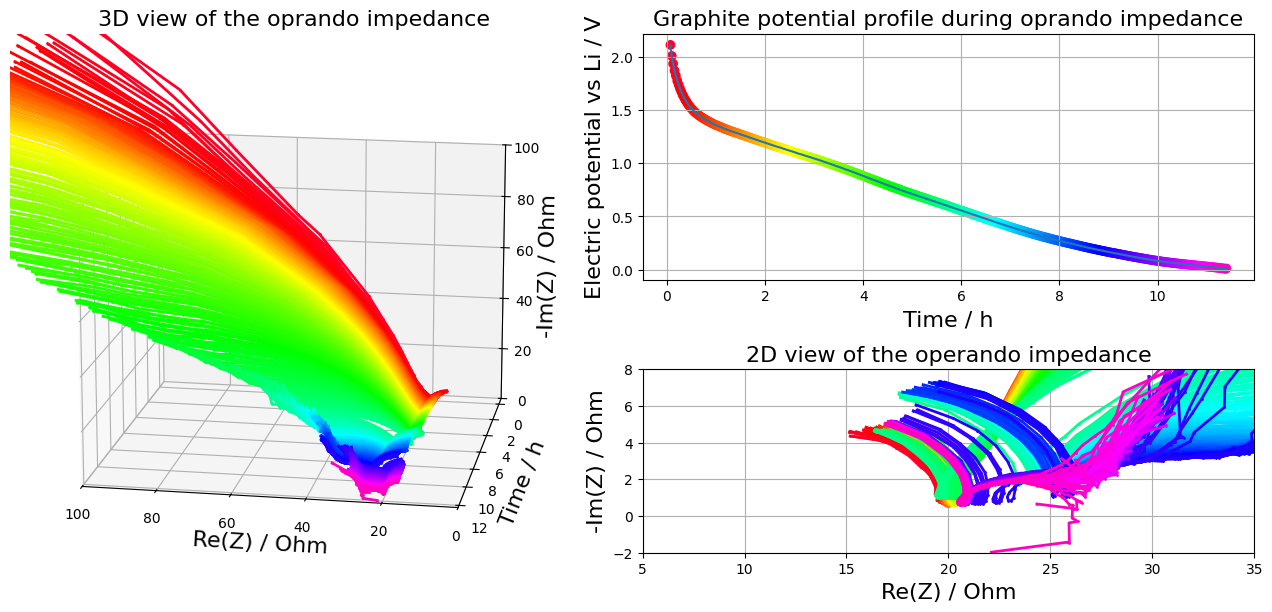
\includegraphics[width = 0.5\textwidth]{figures/anodes/SiCN_pouch39_1.png}
    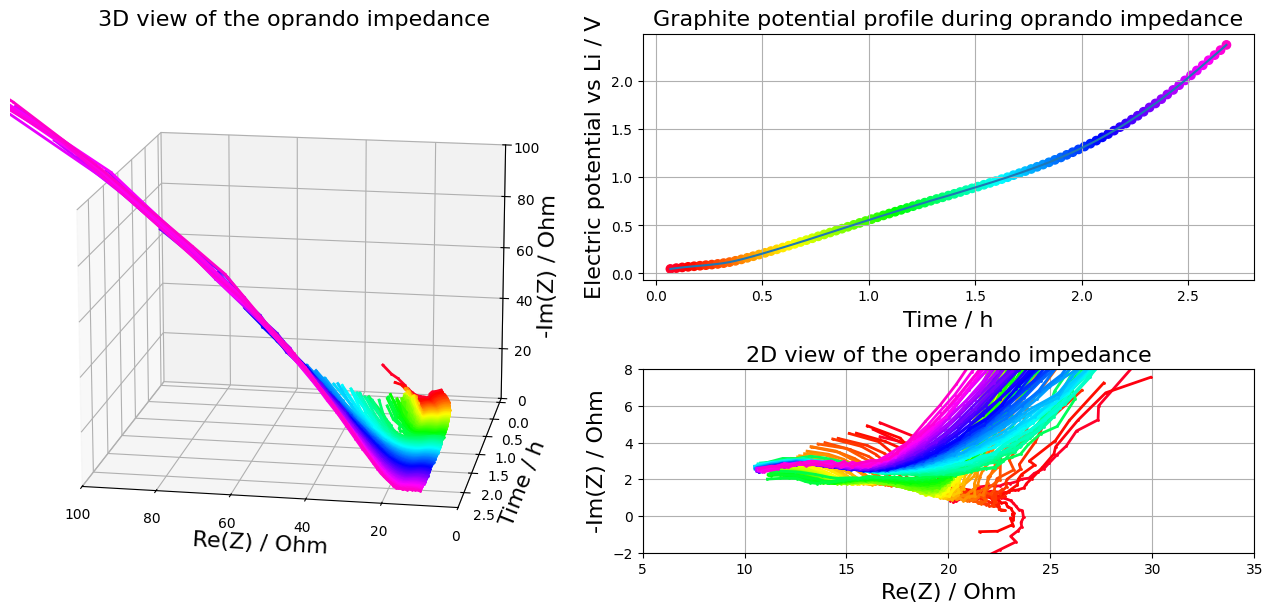
\includegraphics[width = 0.5\textwidth]{figures/anodes/SiCN_pouch39_2.png}
    \caption{Full first cycle of galvanostatic C10 SiCN with DEIS repetition}
    \label{fig:SiCN cell 39 first cycle}
\end{figure}
The formation of SEI is still rapresented in the impedance shape for the same voltage window as before, but then the impedance at high frequencies shows a bigger semicircle. 
On consecutive cicle though, the sudden reduction of the impedance is not observed.
This can be to differences on the porosity of the electrode itself because of the manifacturing process.

\begin{figure}[H]
    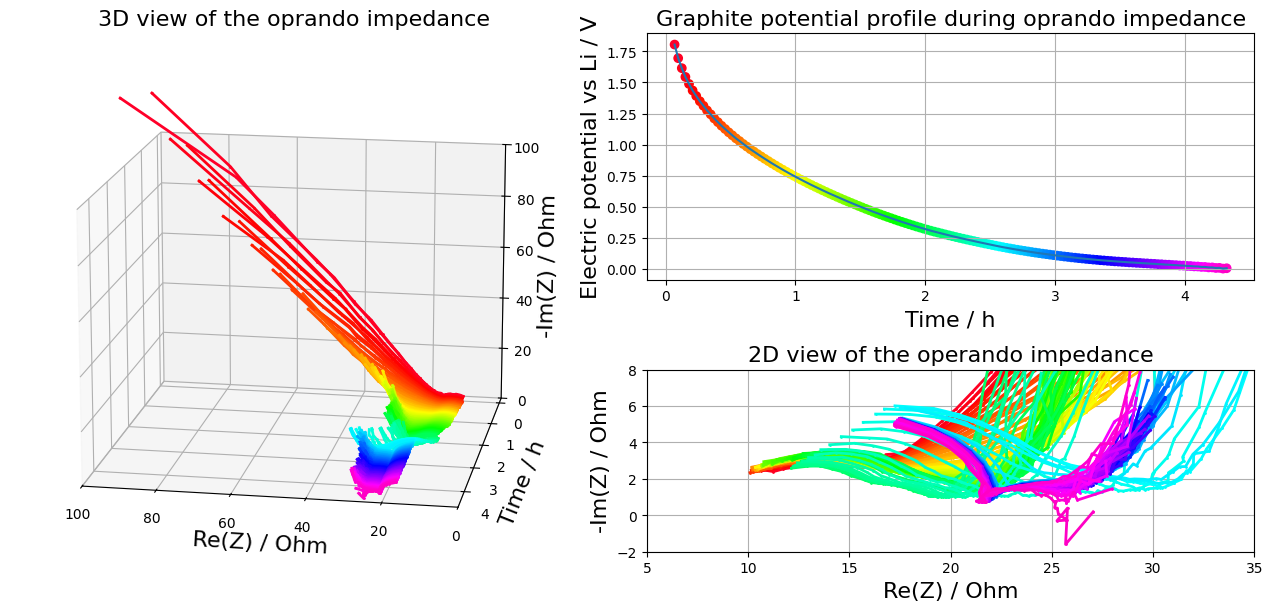
\includegraphics[width = 0.5\textwidth]{figures/anodes/SiCN_pouch39_3.png}
    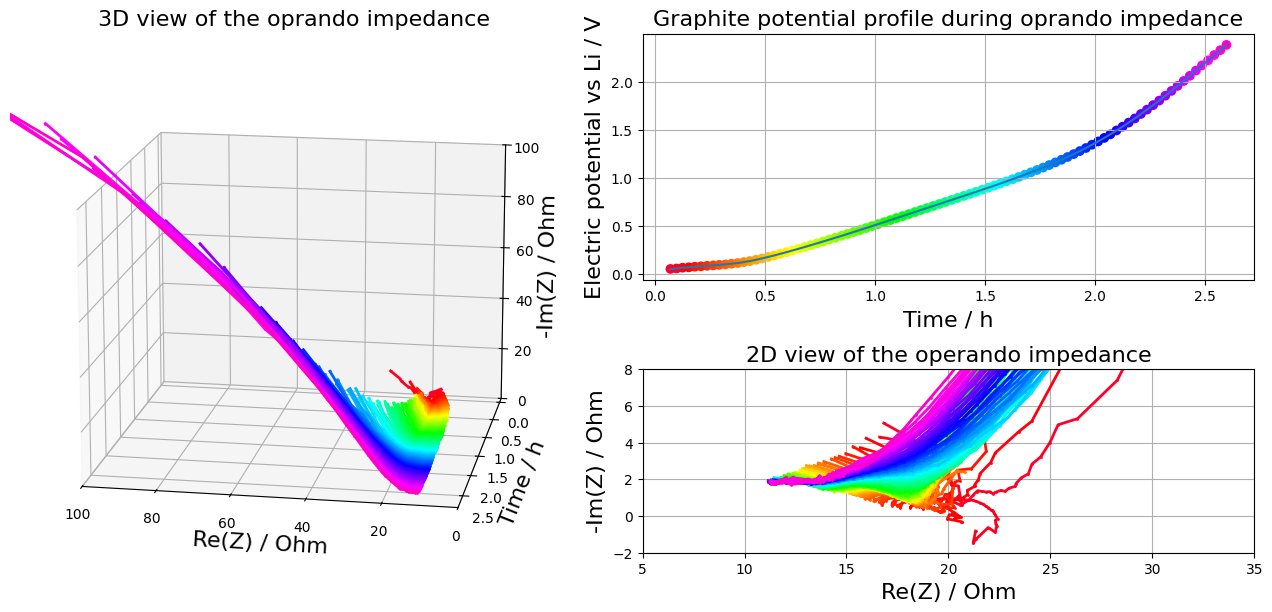
\includegraphics[width = 0.5\textwidth]{figures/anodes/SiCN_pouch39_4.png}
    \caption{Full second cycle of galvanostatic C10 SiCN with DEIS repetition}
    \label{fig:SiCN cell 39 second cycle}
\end{figure}

\begin{figure}[H]
    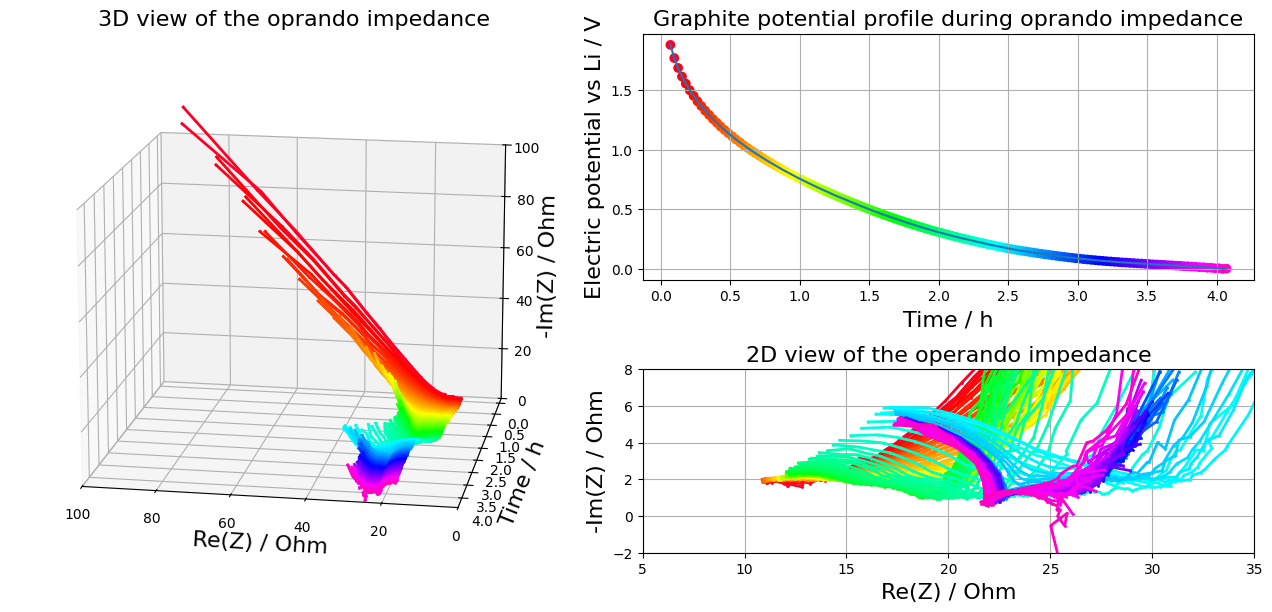
\includegraphics[width = 0.5\textwidth]{figures/anodes/SiCN_pouch39_5.png}
    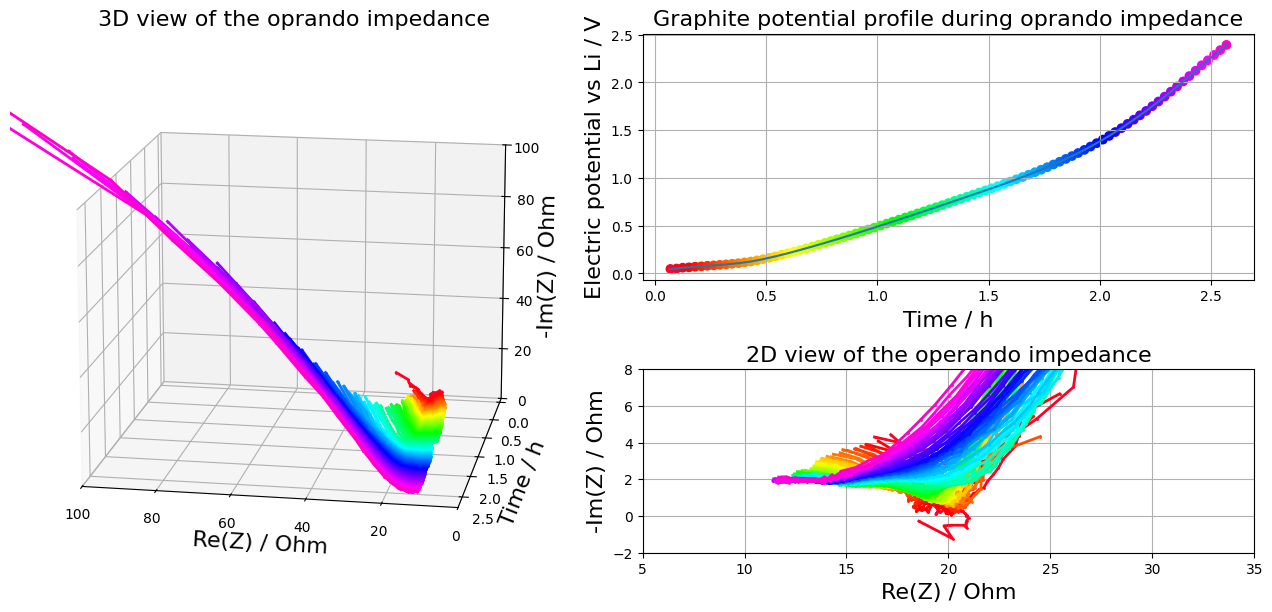
\includegraphics[width = 0.5\textwidth]{figures/anodes/SiCN_pouch39_6.png}
    \caption{Full third cycle of galvanostatic C10 SiCN with DEIS repetition}
    \label{fig:SiCN cell 39 third cycle}
\end{figure}

In both cells, for cathodic carrents I se characteristics shapes of the impedance that jump after certain votlages. 
This could help identify the different storage mechanisms.

To clarify what happens in the high frequency band I should use the automated set-up with online partial impedance calculation that I havn't competed at the time of this experiments.
Furthermore, new experiments require reporducible Silicon Carbonitrate electrodes.

\subsection{Results of Sodium}
% Show impedance and various cycles
% Comment that the shape of the impedance changes with the state of the surface, that could be of geometrical orgin (roughness) or for the presence or formation of the SEI.

I performed this experiment to verify how the impedance behave when depositing sodium on existing sodium.
The question was if we could see again that sudden decrease in impedance or other features.

The cell undergone one hour of electrodeposition with the same current 120uA of the C/10 C-rate for the Silicon Carbonitrate during which the SEI is formed.
Then I left the cell in rest for a few days before performing the  plating and stripping cycles.
The result of the first is shown in figure \ref{fig:Na electrodeposition DEIS}.
\begin{figure}[H]
    \centering
    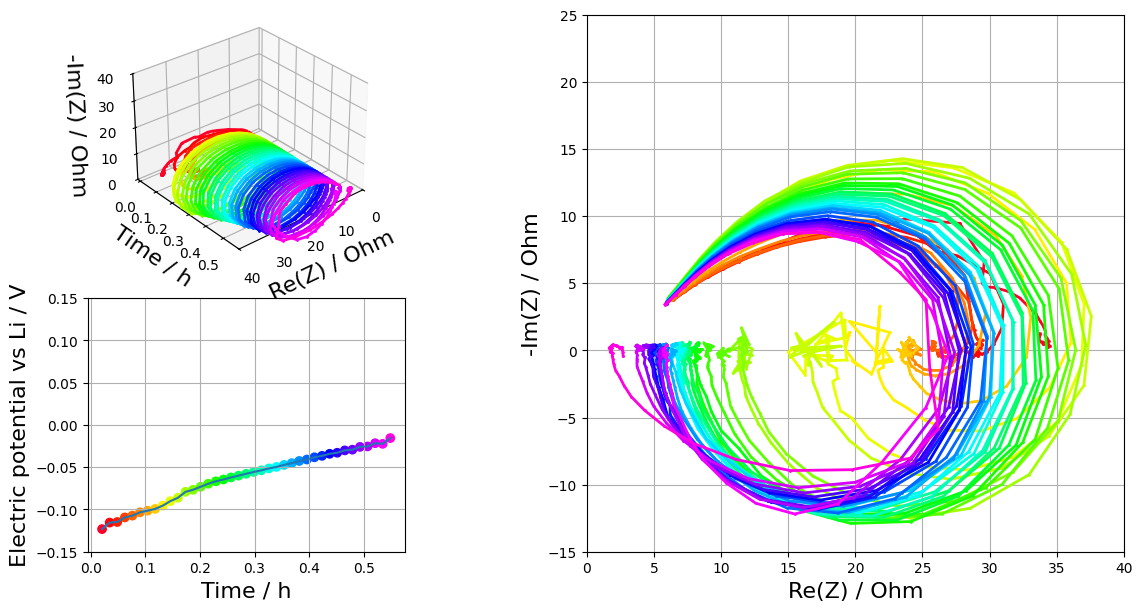
\includegraphics[width = 0.8\textwidth]{figures/anodes/sodium_pouch_1.png}
    \caption{Reduction}
    \label{fig:Na electrodeposition DEIS}
\end{figure}
Immediatly the impedance shows a positive immaginary part. 
A curl that goes back to smaller real resistance values with the increase of impedance.
The overpotential reduces from -120mV to =10mV signaling and increase of surface during deposition. 
This curl to positive immaginry part is observed when the electroreduced species undergoes an intermediate slow step in moving to a nucleation state.
In this Sodium reduction, it seems that the intermadiate step is the limiting reaction step and it might be caused by the presence of the SEI layer, to the rugosisty or the surface or its dendritic structure. 
There is no much reserach in this topic published in the literature.
The measurement was performed for one hour, but in the plot of Dynamic Impednace result only 40 minutes are presented becaus of an error in the data recording (at the time of this measurments I was still prototyping the setup).

When performing the stripping, the impedance looses soon the curly feature moving to a more typycal semicircle.
The reaction is not limited by mass transport since the Warburg diffusion tail is not present.
The persistance of the curl at begging of the step even with anodic current suggests that it is not connected to the type of reaction (reduction of Sodium) but rather the surface morfology.
\begin{figure}[H]
    \centering
    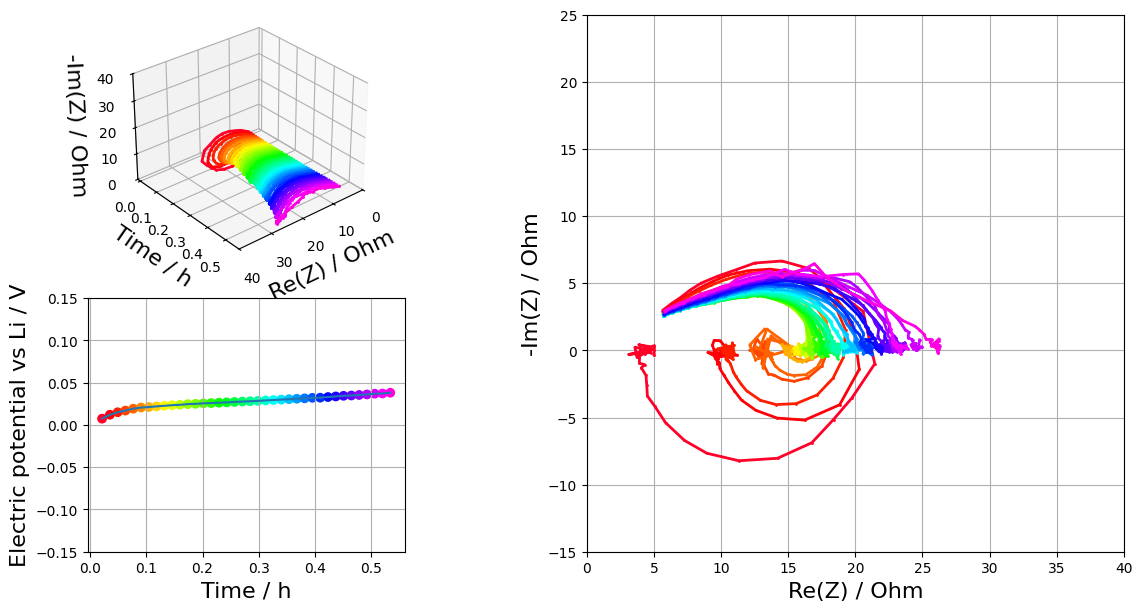
\includegraphics[width = 0.8\textwidth]{figures/anodes/sodium_pouch_2.png}
    \caption{Oxidation}
    \label{fig:Na stripping DEIS}
\end{figure}
The important fact is that the positive impedance curl was observed also in another cell of identical costruction meaning the processes is reproducible altough it depends on the story of the electrode. 
In fect after stripping and the change of surface structure or SEI thickness, the curl is no more present while the overvoltage stays constant around 50mV as reported in Figure \ref{fig:Na second electrodeposition DEIS}
\begin{figure}[H]
    \centering
    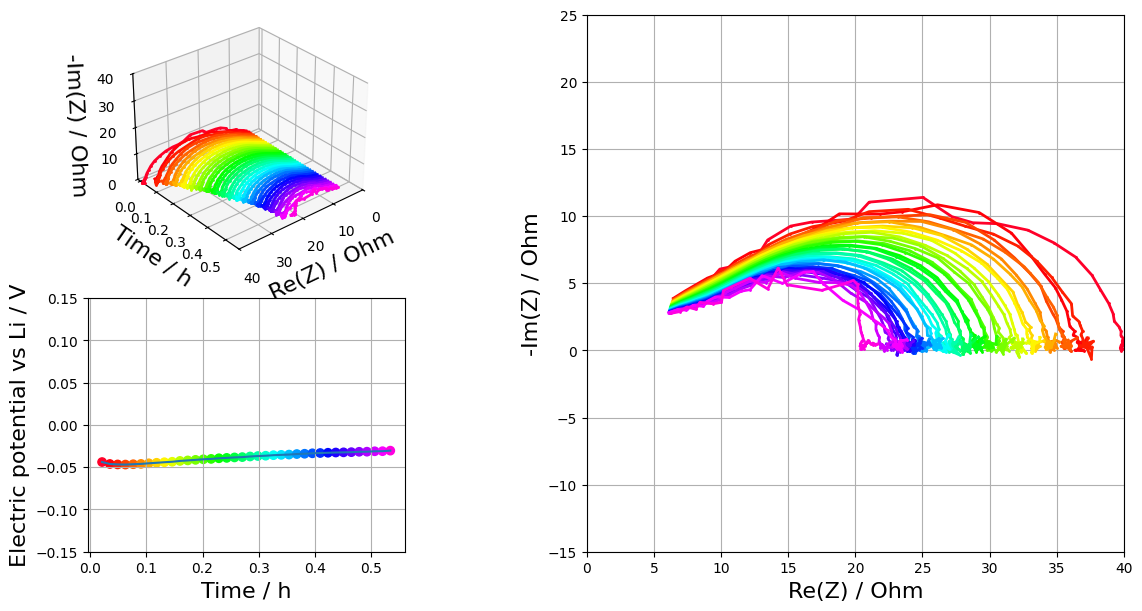
\includegraphics[width = 0.8\textwidth]{figures/anodes/sodium_pouch_3.png}
    \caption{Reduction again}
    \label{fig:Na second electrodeposition DEIS}
\end{figure}

To fully understand the system, it is will be important also here to extend the highest frequency to fully see the behaviour.
Furthermore experiment at different current density would clarify the physics of the system and I would also calculate the deposition efficiency to draw batter conclusion. 
All of these are possible with the latest version of the software I developed, so I envision this as future research project.

I also noticed that the last frequency points have the same impedance value (plus noise) so I could have removed at least one decade of frequency point, if not two. 
I wander if this experiment could be possible with a classic single frequency measurement using the Frequency Respone Analyzer. 

\section{Majour problematics of this work}
Data is partial and some cycles or electrode hystory are missing due to the sevelopment process of the software in parallel to these (secondary) projects.
I didn't have the time to increse my expertese in fabricating micro-refernece electrodes or find other routs to prepare them, leading to absense of reproducibile results to confirm the supposition of deposition. 
Impedance is very sensitive to electrode surface so the electrode must be identical or a wide number of experiment is needed to widrow sounding conlsusions.
The sealing of the pouch cell could also be problematic, introducing air that drives side-reaction. 
In fact, I found later an open pouch bag for the failing of the sealing.
Furthermore, this types of microrefrence electrode are still too thick.
In fact they are af the same thickness of the electodes themselves (50um for the smaller wire). 
This probably introduce deformation of the planarity of the electrode even when using the flexbile glass fiber separators and this is particluarly important for small area alectrode like the ones used here.
Alternative electrodes could be based on intercalation materials like lithium Iron Posphate as often reported in the literature [cite papres] and usng metallic grid as support could avoid the deformation.

\section{Summary and perspectives}
% What worked
This chapter shows that DEIS reveals mechnistic information of the storage mechanisms for battery negative electrode active materials: graphite for the intercalation of Lithium and SiCN(O) for the intercalation of Sodium. THe istantanous impedance shows in both cases the presence of electrochemical processes such as SEI formation, phase change (as alredy pointed out in chapter \ref{chap:capacitor}) and a peculiar temporary reduction of impedance. This phenomenon is observed in both graphite and SiCN(O) and I speculate being overpotential metal deposition.
% What didn't work (reproducibility, amplitude change during cycling)

% What should be imporoved? (Geometry, RE production, pouch geometry, ecc.)
The contact between microscopic wires and metallic current collector tabs must be improved using other soldering methods (conducitve silver glue or microscopic soldering).
% why the results are still valuable (do not oversell):
The result remain still valuable in the sense that they lead to the possiblity of identify processes in-situ during the operation of the device that would not have been possible with static impedance. Dynamic processes like SEI formation can be trakced with this method or processes induced by the operating conditions such as metal deposition can be istantanously identified.
% -early impedance signatures of plating or SEI
% -demonstration of DEIS feasibility in 3-electrode pouch cells
% -lessons for future studies